%=============================================================================%
% RAPPORT PFE - Attijariwafa Bank / ESI
%=============================================================================%

\documentclass[11pt,a4paper,twoside]{report}

%------------------------------------------------------------------------------%
% PAQUETS
%------------------------------------------------------------------------------%
\usepackage{titlesec}
\titlespacing*{\section}{0pt}{1ex plus 0ex minus 0ex}{0.5ex plus 0ex minus 0ex}
\titlespacing*{\subsection}{0pt}{1ex plus 0ex minus 0ex}{0.5ex plus 0ex minus 0ex}
\usepackage{placeins}
\usepackage[utf8]{inputenc}
\usepackage[T1]{fontenc}
\usepackage[french]{babel}
\usepackage{geometry}
\usepackage{graphicx}
\usepackage{fancyhdr}
\usepackage{tocloft}
\usepackage{setspace}
\usepackage{xcolor}
\usepackage{booktabs}
\usepackage{float}
\usepackage{caption}
\usepackage{subcaption}
\usepackage{array}
\usepackage{longtable}
\usepackage{enumitem}
\usepackage{tabularx}
\usepackage{pgfgantt}
\usepackage{rotating}
\usepackage{pdflscape}
\usepackage{svg}
\usepackage[table]{xcolor}
\usepackage[hidelinks]{hyperref}
\AtBeginDocument{%
  \renewcommand{\listfigurename}{Liste des figures}%
  \renewcommand{\listtablename}{Liste des tableaux}%
}
%------------------------------------------------------------------------------%
% MISE EN PAGE
%------------------------------------------------------------------------------%
\geometry{left=2.5cm,right=2.5cm,top=2.5cm,bottom=2.5cm}
\setstretch{1.15}
\setlength{\headheight}{14pt}

\pagestyle{fancy}
\fancyhf{}
\lhead{\leftmark}
\rhead{\thepage}
\renewcommand{\headrulewidth}{0.4pt}
\renewcommand{\footrulewidth}{0pt}

\titleformat{\chapter}[display]
  {\normalfont\bfseries\Large}{\chaptertitlename\ \thechapter}{20pt}{\Huge}
\titlespacing*{\chapter}{0pt}{12pt}{20pt}

\titleformat{\section}
  {\normalfont\large\bfseries}{\thesection}{1em}{}
\titleformat{\subsection}
  {\normalfont\normalsize\bfseries}{\thesubsection}{1em}{}
\titleformat{\subsubsection}
  {\normalfont\normalsize\itshape}{\thesubsubsection}{1em}{}

%------------------------------------------------------------------------------%
% COULEURS
%------------------------------------------------------------------------------%
\definecolor{backcolour}{rgb}{0.95,0.95,0.95}
\definecolor{attired}{RGB}{204,27,27}

% Macro pour les espaces réservés aux images
\newcommand{\imageplaceholder}[3]{%
\begin{figure}[H]
    \centering
    \fbox{\parbox[c][#2][c]{0.92\textwidth}{\centering
        \vspace{0.15cm}
        \textbf{[IMAGE A INSERER]}\\[0.25cm]
        \small\textit{#3}
        \vspace{0.15cm}
    }}
    \caption{#1}
\end{figure}
}

% Helper: compact itemize inside table cells
\newlist{tblitem}{itemize}{1}
\setlist[tblitem]{leftmargin=0.5cm, nosep, topsep=2pt, itemsep=1pt, parsep=0pt, before=\vspace{2pt}, after=\vspace{2pt}}

\begin{document}

%=============================================================================%
% PAGE DE GARDE
%=============================================================================%
\begin{titlepage}
    \thispagestyle{empty}
    \centering

    % --- En-tête : logos écartés aux bords, organisme centré ---
    \noindent
    \begin{tabular}{@{}p{0.18\textwidth}p{0.64\textwidth}p{0.18\textwidth}@{}}
        \raggedright \hspace*{-0.8cm}
\includegraphics[height=1.5cm]{logoesi.jpg}
        &
        \centering
        {\large Royaume du Maroc}\\[0.15cm]
        {\normalsize Haut-Commissariat au Plan}
        &
        \raggedleft \hspace*{-0.8cm}
\includegraphics[height=1.5cm]{logoawb.png}
        \tabularnewline
    \end{tabular}

    \vspace{2cm}

    % --- Cadre titre ---
    \fbox{
        \parbox{0.85\textwidth}{
            \centering
            \vspace{0.4cm}
            {\LARGE \textbf{Développement d'une plateforme d'intelligence territoriale pour l'optimisation du réseau d'agences bancaires}}
            \vspace{0.4cm}
        }
    }

    \vspace{2cm}

    {\large Mémoire de Fin d'Études présenté pour l'obtention}\\[0.2cm]
    {\large du diplôme d'Ingénieur d'État}\\[0.2cm]
    {\large de l'École des Sciences de l'Information}

    \vspace{1.8cm}

    {\large \textbf{SALAH EDDINE AHADAF}}

    \vspace{1.2cm}

    {\large Sous la direction de Pr. Basma Boukenze}

    \vspace{2cm}

    \begin{tabular}{ll}
        \hspace*{-2.8cm}\textbf Membres du jury: \\[0.3cm]
        \hspace*{-2cm}\textbf Président : & Pr Jaouad Maqboul \\[0.3cm]
        \hspace*{-2cm}\textbf Encadrant : & Pr Basma Boukenze \\[0.3cm]
        \hspace*{-2cm}\textbf Tuteur : & M Ahmed EL Rheddane \\
    \end{tabular}

    \vspace{4cm}

    {\large Année universitaire~: 2025/2026}

\end{titlepage}

%------------------------------------------------------------------------------%
% DÉDICACE
%------------------------------------------------------------------------------%
\pagenumbering{roman}
\chapter*{Dédicace}
\addcontentsline{toc}{chapter}{Dédicace}

\vspace{1cm}

\begin{center}
\textit{Avec l'expression de ma profonde reconnaissance, je dédie ce travail à ceux à qui, quels que soient les termes employés, je n'arriverai jamais à exprimer mon amour sincère.}
\end{center}

\vspace{0.5cm}

\textbf{À mes chers parents,} pour leur patience, leur soutien, leur affection et leurs sacrifices constants ; vous êtes ma source éternelle d'inspiration, de motivation, de bénédiction, de patience et de persévérance. Aucune expression, aussi éloquente soit-elle, ne saurait traduire pleinement ma gratitude.

\vspace{0.4cm}

\textbf{À mes frères et mes sœurs,} qui m'ont toujours soutenu et encouragé tout au long de mes études ; vous m'avez inculqué le sens de la responsabilité, de l'optimisme et de la confiance en moi.

\vspace{0.4cm}

\textbf{À mes chers amis,} pour leur confiance et leur appui inestimable ; vous avez guidé mes pas vers la réussite par vos conseils et votre affection.

\vspace{0.4cm}

\textbf{À tous ceux qui me sont chers ;} à vous tous, merci d'avoir toujours été à mes côtés et d'avoir partagé avec moi chaque étape de ce parcours.

\newpage

%------------------------------------------------------------------------------%
% REMERCIEMENTS
%------------------------------------------------------------------------------%

\chapter*{Remerciements}
\addcontentsline{toc}{chapter}{Remerciements}

\vspace{1cm}

Avant d'entamer ce rapport de projet de fin d'études, je présente mes remerciements les plus vifs et ma reconnaissance la plus sincère à tous ceux qui m'ont aidé et soutenu durant ce parcours.

Mes remerciements les plus respectueux vont à mon encadrante académique, \textbf{Mme Basma Boukenze}, professeure à l'École des Sciences de l'Information (ESI), qui m'a fait l'honneur de superviser ce travail ; qu'elle trouve ici l'expression de ma profonde reconnaissance pour son encadrement, sa patience, ses conseils et sa disponibilité continue tout au long de la réalisation de ce projet.

J'adresse également mes vifs remerciements à mon encadrant d'entreprise, \textbf{M. Ahmed El Rheddane}, chez Attijariwafa Bank, pour ses précieux conseils, sa disponibilité et la confiance qu'il m'a accordée tout au long de cette période de stage au sein du Digital Center. Il m'a encadré et soutenu avec beaucoup de professionnalisme et de savoir-faire.

Je remercie aussi l'ensemble des équipes d'Attijariwafa Bank, pour leur sympathie, leurs conseils et l'environnement de travail propice qu'ils ont su créer, facilitant ainsi la bonne marche de ce projet.

Enfin, j'exprime ma profonde gratitude au corps professoral et administratif de \textbf{l'École des Sciences de l'Information (ESI)}, ainsi qu'à tous ceux qui m'ont aidé ou encadré pour me transmettre leurs savoirs dans les meilleures conditions possibles.

\newpage

%------------------------------------------------------------------------------%
% RÉSUMÉ
%------------------------------------------------------------------------------%

\chapter*{Résumé}
\addcontentsline{toc}{chapter}{Résumé}

\vspace{1cm}

Ce rapport présente le travail réalisé dans le cadre d'un projet de fin d'études mené au sein d'Attijariwafa Bank, visant à construire une plateforme d'Intelligence Territoriale d'aide à la décision pour l'optimisation du réseau d'agences bancaires sur l'ensemble du territoire marocain. L'objectif central est d'évaluer objectivement la performance des agences existantes en isolant leur potentiel géographique de leur exécution managériale, et de sélectionner de nouveaux emplacements à fort potentiel.

Pour répondre à ce besoin, une approche combinant plusieurs techniques avancées d'analyse spatiale et de Machine Learning a été mise en place. D'une part, la collecte et le traitement de données massives (Points d'Intérêt via OpenStreetMap et Overture Maps, densité de population) permettent de créer un scoring géospatial normalisé de l'environnement de chaque agence. D'autre part, un pipeline d'apprentissage automatique dynamique (Auto-ML intégrant XGBoost et Random Forest) est utilisé pour modéliser la relation entre le potentiel géographique et les revenus financiers.

La plateforme intègre deux fonctionnalités majeures : une analyse des écarts ("Gap Analysis") projetée sur une matrice stratégique, permettant de catégoriser les agences (Excellence, À surveiller, À revoir, À fermer) et de proposer des fusions géospatiales intelligentes ; et un algorithme de similarité cosinus vectorisée pour comparer des millions de sites candidats aux agences les plus performantes, facilitant la sélection de nouveaux emplacements.

Les résultats obtenus montrent que cette solution interactive et paramétrable fournit un tableau de bord complet et intuitif. Elle permet aux décideurs métiers de visualiser la restructuration spatiale du réseau, de télécharger des recommandations actionnables et d'optimiser la stratégie d'implantation territoriale avec précision.

\vspace{\fill}
\noindent\rule{\textwidth}{0.4pt} \\
\textbf{Mots clés :} Intelligence Territoriale, Machine Learning, Analyse Spatiale, Optimisation du réseau bancaire, Scoring Géospatial, Attijariwafa Bank.

\newpage

\chapter*{Abstract}
\addcontentsline{toc}{chapter}{Abstract}

\vspace{1cm}

This report presents the work carried out as part of an end-of-studies project conducted at Attijariwafa Bank, aiming to build a Territorial Intelligence decision-support platform for optimizing the bank branch network across the entire Moroccan territory. The central objective is to objectively evaluate the performance of existing branches by isolating their geographic potential from their managerial execution, and to select new high-potential locations.

To meet this need, an approach combining several advanced spatial analysis and Machine Learning techniques was implemented. On one hand, the collection and processing of massive data (Points of Interest via OpenStreetMap and Overture Maps, population density) allow for the creation of a normalized geospatial scoring of each branch's environment. On the other hand, a dynamic machine learning pipeline (Auto-ML integrating XGBoost and Random Forest) is used to model the relationship between geographic potential and financial revenues.

The platform integrates two major features: a gap analysis projected onto a strategic matrix, allowing to categorize branches (Excellence, To monitor, To review, To close) and propose intelligent geospatial mergers; and a vectorized cosine similarity algorithm to compare millions of candidate sites to the best-performing branches, facilitating the selection of new locations.

The obtained results show that this interactive and customizable solution provides a comprehensive and intuitive dashboard. It allows business decision-makers to visualize the spatial restructuring of the network, download actionable recommendations, and optimize the territorial expansion strategy with precision.

\vspace{\fill}
\noindent\rule{\textwidth}{0.4pt} \\
\textbf{Keywords :} Territorial Intelligence, Machine Learning, Spatial Analysis, Bank Network Optimization, Geospatial Scoring, Attijariwafa Bank.

\newpage

%------------------------------------------------------------------------------%
% TABLE DES MATIÈRES
%------------------------------------------------------------------------------%
\tableofcontents
\newpage

\addcontentsline{toc}{chapter}{Liste des figures}
\listoffigures
\newpage

\addcontentsline{toc}{chapter}{Liste des tableaux}
\listoftables
\newpage

%------------------------------------------------------------------------------%
% LISTE DES ACRONYMES
%------------------------------------------------------------------------------%
\pagenumbering{arabic}
\chapter*{Liste des acronymes}
\addcontentsline{toc}{chapter}{Liste des acronymes}

\begin{tabular}{@{}lp{11cm}@{}}
\toprule
\textbf{Acronyme} & \textbf{Définition} \\
\midrule
API    & Application Programming Interface \\
AWB    & Attijariwafa Bank \\
BI     & Business Intelligence \\
CSV    & Comma-Separated Values \\
DBSCAN & Density-Based Spatial Clustering of Applications with Noise \\
ESI    & École des Sciences de l'Information \\
ETL    & Extract, Transform, Load \\
GIS    & Geographic Information System \\
GPS    & Global Positioning System \\
KMeans & K-Means Clustering \\
KPI    & Key Performance Indicator \\
ML     & Machine Learning \\
OSM    & OpenStreetMap \\
OMF    & Overture Maps Foundation \\
PCA    & Principal Component Analysis \\
PFE    & Projet de Fin d'Études \\
POI    & Point of Interest (Point d'Intérêt) \\
SQL    & Structured Query Language \\
UI     & User Interface \\
UX     & User Experience \\
UML    & Unified Modeling Language) \\
Auto-ML& Automated Machine Learning \\
BCG    & Boston Consulting Group \\
XGBoost& eXtreme Gradient Boosting \\
cKDTree& C-based K-Dimensional Tree \\
JSON   & JavaScript Object Notation \\
\bottomrule
\end{tabular}

\newpage

%=============================================================================%
% INTRODUCTION GÉNÉRALE
%=============================================================================%
\chapter*{Introduction Générale}
\addcontentsline{toc}{chapter}{Introduction Générale}

Dans le contexte actuel de transformation numérique, les données occupent une place centrale dans le fonctionnement et la compétitivité des institutions financières. Que ce soit dans le secteur bancaire, la gestion patrimoniale ou les services financiers, la capacité à collecter, traiter et analyser des volumes importants d'informations géographiques et commerciales est devenue un enjeu stratégique de premier plan. Cette évolution, portée par la multiplication des sources numériques comme les points d'intérêt cartographiques, les transactions bancaires ou les indicateurs de performance, oblige les organisations financières à repenser leurs outils d'aide à la décision.

Face à cette réalité, les méthodes traditionnelles de sélection d'emplacement bancaire, basées sur des critères subjectifs et des processus souvent manuels, montrent aujourd'hui clairement leurs limites. Elles peinent à suivre la croissance rapide des réseaux, à tenir compte de la diversité des environnements urbains et ruraux, et à produire des analyses rapides et fiables. De nouvelles approches, combinant l'apprentissage automatique et la géolocalisation, émergent pour combler ce manque. Elles offrent une réponse plus adaptée aux exigences actuelles de l'expansion bancaire.

C'est dans ce contexte que s'inscrit ce stage de fin d'études, réalisé au sein d'Attijariwafa Bank. Le projet consiste à concevoir et mettre en place une plateforme d'intelligence territoriale dédiée à l'analyse du réseau d'agences bancaires. L'objectif est de fournir un outil capable d'évaluer et de comparer les agences existantes sur l'ensemble du territoire marocain, d'identifier les zones de redondance et les candidats à la fermeture ou à la fusion, et de recommander les meilleurs emplacements pour de nouvelles ouvertures. Pour cela, la plateforme s'appuie sur plusieurs scores normalisés construits à partir de l'environnement immédiat de chaque agence : score commercial, score bureaux, score résidentiel, accessibilité, concurrence et cannibalisation.

La solution technique repose sur une architecture modulaire, intégrant la collecte de points d'intérêt depuis plusieurs sources cartographiques, des algorithmes de clustering et de similarité vectorielle, et un tableau de bord interactif développé avec les outils Python les plus adaptés. Cette approche vise à produire des résultats précis, reproductibles et directement exploitables par les responsables métier.

Le rapport est organisé en plusieurs chapitres. Le premier présente le contexte du projet, la banque, la problématique et les objectifs fixés. Le deuxième décrit la conception fonctionnelle et les choix d'architecture de données. Le troisième détaille la conception technique, les algorithmes retenus et les outils utilisés. Le quatrième chapitre présente la réalisation concrète avec les résultats obtenus, les limites identifiées et les perspectives d'amélioration.

%=============================================================================%
% CHAPITRE 1 : CONTEXTE DU PROJET
%=============================================================================%
\chapter{Contexte du Projet}

\section{Présentation de l'Organisme d'Accueil}

Ce premier chapitre a pour but de présenter le cadre général dans lequel ce stage de fin d'études a été effectué. On va commencer par présenter Attijariwafa Bank, l'institution qui nous a accueillis, en donnant ses informations essentielles, ses chiffres clés et son histoire. Ensuite, on va présenter le projet lui-même : son contexte, le problème auquel il répond, les objectifs qu'on s'est fixés et la façon dont on a organisé le travail.

Cette présentation permet de bien comprendre pourquoi ce projet a été lancé, dans quel environnement il a été réalisé, et quelles contraintes il devait respecter. Elle prépare aussi à lire les chapitres suivants en donnant les repères nécessaires.

\section{Présentation d'Attijariwafa Bank}

Attijariwafa Bank est le premier groupe bancaire et financier au Maroc et l'un des plus importants du continent africain. Il est présent dans 26 pays à travers l'Afrique, l'Europe et le Moyen-Orient, et accompagne aujourd'hui plus de 12 millions de clients, qu'il s'agisse de particuliers, de professionnels, d'entreprises ou d'institutions.

Le groupe propose une gamme complète de services financiers : banque de détail, banque d'entreprise, financement, assurance, gestion d'actifs et services spécialisés. Cette diversité en fait un acteur incontournable dans le paysage économique marocain et africain.

Avec un réseau de plus de 4 300 agences à l'échelle du groupe, dont environ 1 196 au Maroc, et plus de 20 000 collaborateurs dans le monde, Attijariwafa Bank représente une organisation dont la gestion du réseau physique est un enjeu quotidien majeur. C'est dans cette logique que le projet prend tout son sens.

\begin{figure}[ht]
    \centering
    
\includegraphics[width=0.35\textwidth]{logoawb.png}
    \caption{AWB}
    \label{fig:my_image}
\end{figure}

\subsection{La Fiche Signalétique}

La fiche signalétique regroupe les informations administratives et générales sur l'organisme d'accueil.

\begin{table}[H]
\centering
\small
\renewcommand{\arraystretch}{1.35}
\rowcolors{1}{orange!50}{orange!15}
\begin{tabular}{|p{4.5cm}|p{8.5cm}|}
\hline
\textbf{Désignation} & \textbf{Valeur} \\
\hline
Nom commercial & Attijariwafa Bank \\
\hline
Forme juridique & Société Anonyme à Conseil d'Administration \\
\hline
Siège social & 2, Boulevard Moulay Youssef, Casablanca 20000, Maroc \\
\hline
Site de stage & Rue Yaacoub El Mansour, Rabat, Maroc \\
\hline
Site web & \texttt{www.attijariwafabank.com} \\
\hline
Capital social & 2 151 408 390 DH \\
\hline
Registre de commerce & N° 333 (Casablanca) \\
\hline
Président Directeur Général & Mohamed El Kettani \\
\hline
Secteur d'activité & Services bancaires et financiers \\
\hline
Présence internationale & 26 pays (Afrique, Europe, Moyen-Orient) \\
\hline
\end{tabular}
\caption{Fiche signalétique d'Attijariwafa Bank}
\end{table}

\subsection{Historique d'Attijariwafa Bank}

Attijariwafa Bank est née en 2004 de la fusion de deux banques marocaines historiques : la Banque Commerciale du Maroc (BCM) et Wafabank. Cette fusion a créé le premier groupe bancaire privé du pays, avec un réseau déjà important et une base de clients solide.

Les origines des deux entités fondatrices remontent bien plus loin. Wafabank hérite d'une histoire qui commence en 1904, lorsque la Compagnie Française de Crédit et de Banque a ouvert une agence à Tanger. La BCM, de son côté, trouve ses racines en 1911 avec l'installation d'une branche de la Banque Transatlantique, également à Tanger.

Depuis 2004, le groupe a connu une expansion progressive et régulière. Il a renforcé sa présence au Maroc, développé ses filiales africaines et intégré plusieurs acquisitions dans différents pays. En 2005, il entre en Tunisie avec l'acquisition d'une participation dans la Banque du Sud, rebaptisée Attijari Bank. En 2008 et 2009, plusieurs autres banques africaines rejoignent le groupe au Sénégal, en Côte d'Ivoire, au Congo, au Gabon et au Mali.

Mohamed El Kettani dirige le groupe depuis 2007 et a conduit plusieurs plans stratégiques successifs. Le plan actuel, "@MBITIONS 2025", lancé en 2021, vise à renforcer le leadership continental de la banque, à accélérer la transformation digitale et à améliorer l'efficacité opérationnelle.

\begin{table}[H]
\centering
\small
\renewcommand{\arraystretch}{1.35}
\rowcolors{1}{orange!50}{orange!15}
\begin{tabular}{|p{2.5cm}|p{10cm}|}
\hline
\textbf{Période} & \textbf{Événement clé} \\
\hline
1904 & Création à Tanger de la Compagnie Française de Crédit et de Banque (ancêtre de Wafabank) \\
\hline
1911 & Implantation de la Banque Transatlantique à Tanger (ancêtre de la BCM) \\
\hline
1985 & Changement de nom, naissance de Wafabank \\
\hline
2004 & Fusion BCM et Wafabank : naissance d'Attijariwafa Bank \\
\hline
2005 & Acquisition en Tunisie, début de l'expansion africaine \\
\hline
2007 & Mohamed El Kettani prend la direction du groupe \\
\hline
2008--2010 & Acquisitions en Afrique subsaharienne (Sénégal, Côte d'Ivoire, Congo, Gabon, Mali) \\
\hline
2021 & Lancement du plan stratégique \textit{@MBITIONS 2025} \\
\hline
\end{tabular}
\caption{Grandes étapes de l'histoire d'Attijariwafa Bank}
\end{table}

\subsection{Les Chiffres Clés}

Attijariwafa Bank affiche des indicateurs qui témoignent de son importance dans le secteur financier africain. Ces chiffres montrent à quel point la gestion du réseau physique est une question stratégique pour le groupe.

\begin{table}[H]
\centering
\small
\renewcommand{\arraystretch}{1.35}
\rowcolors{1}{orange!50}{orange!15}
\begin{tabular}{|p{5.5cm}|p{4cm}|p{3cm}|}
\hline
\textbf{Indicateur} & \textbf{Valeur} & \textbf{Portée} \\
\hline
Nombre d'agences au Maroc & Environ 1 196 & National \\
\hline
Réseau total du groupe & Plus de 4 300 agences & Groupe \\
\hline
Nombre de clients & Plus de 12 millions & Groupe \\
\hline
Collaborateurs & Plus de 20 000 & Groupe \\
\hline
Pays de présence & 26 pays & International \\
\hline
Bénéfice net 2023 & 7,5 milliards de DH & Groupe \\
\hline
Produit net bancaire 2023 & 29,9 milliards de DH & Groupe \\
\hline
Capital social & 2,15 milliards de DH & Groupe \\
\hline
\end{tabular}
\caption{Chiffres clés d'Attijariwafa Bank (données 2023--2024)}
\end{table}

Ces données montrent clairement qu'un réseau de cette taille nécessite des outils d'analyse performants pour accompagner les décisions liées à l'implantation, à la consolidation ou à la fermeture d'agences.

\begin{figure}[htbp]
    \centering
    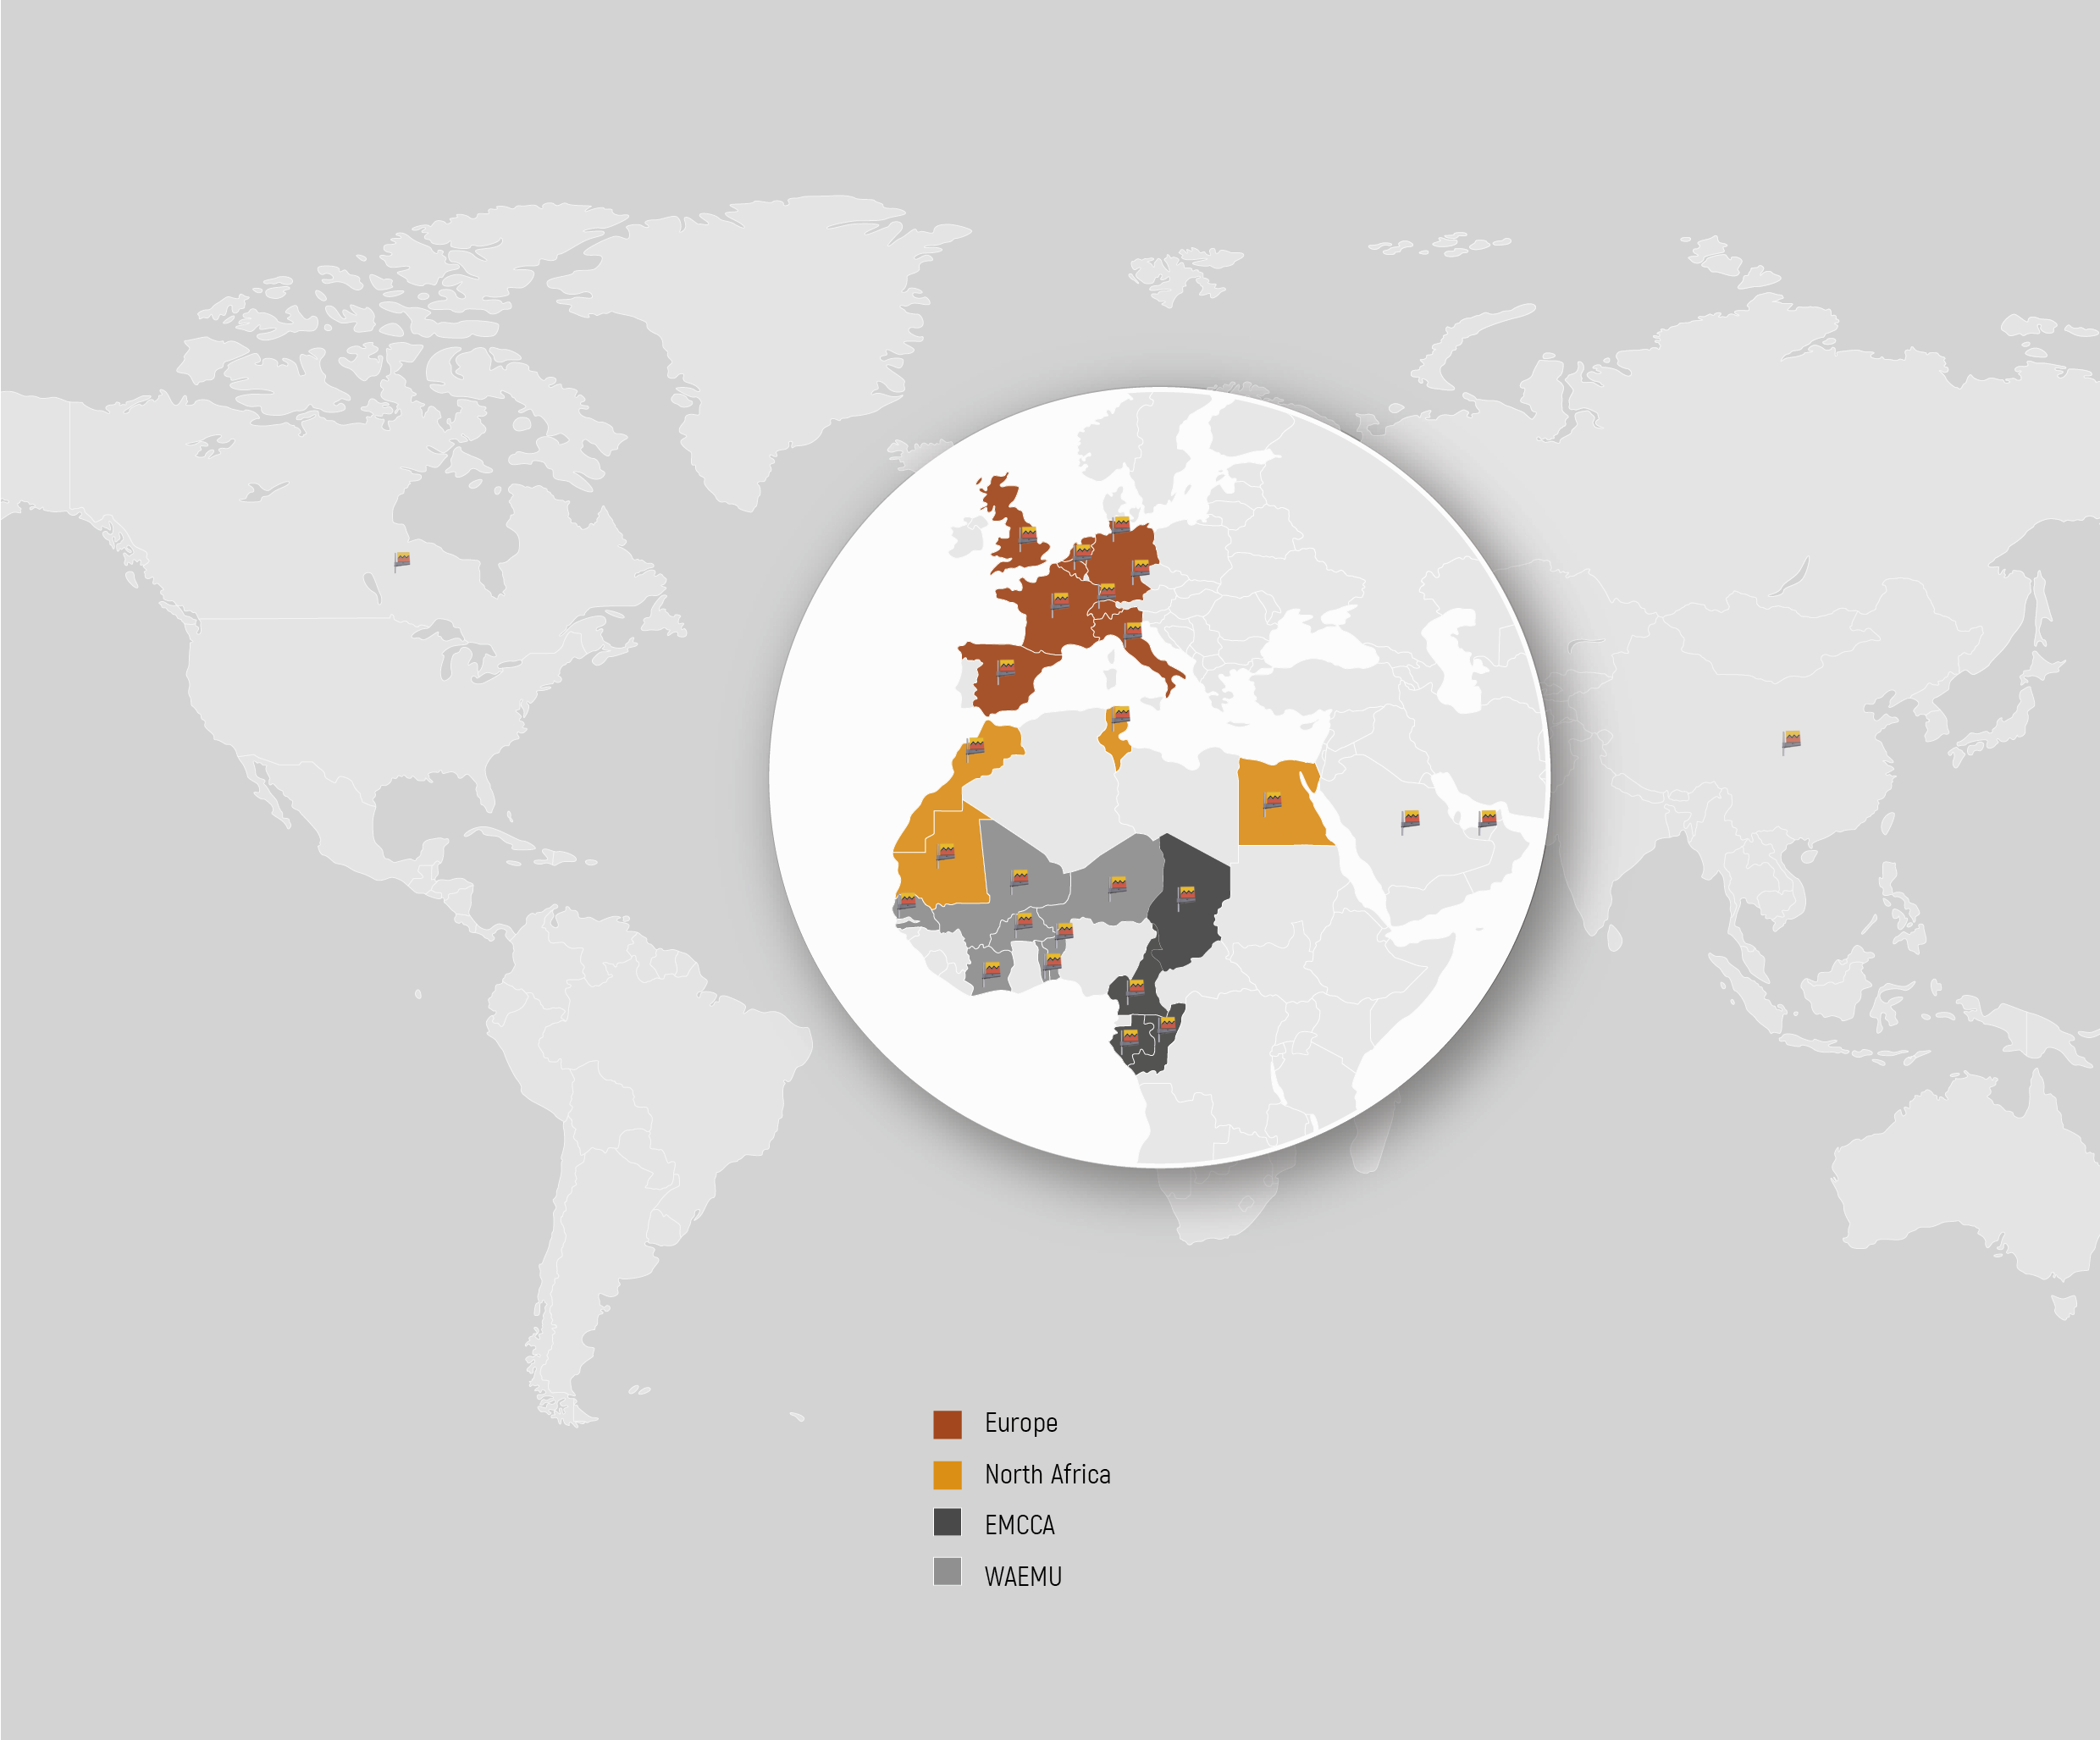
\includegraphics[width=0.5\textwidth]{filiale-mondiale.png}
    \caption{FILIALES MONDIALES}
    \label{fig:filiales}
\end{figure}

\subsection{Pôle Transformation, Innovation, Technologies et Opérations}

Le pôle Transformation, Innovation, Technologies et Opérations (TITO) est l'une des directions centrales du groupe. Il est chargé de piloter la modernisation des systèmes d'information, de gouverner la donnée et de déployer les projets technologiques au service des métiers.

Ce pôle joue un rôle clé dans la transformation numérique de la banque. Il est notamment impliqué dans les projets liés à la qualité des données, à l'automatisation des processus et au développement des outils d'aide à la décision. C'est dans ce cadre que le projet de plateforme d'intelligence territoriale prend sa place : il s'inscrit directement dans la logique de valorisation de la donnée pour appuyer les décisions stratégiques du réseau.

Mon stage s'est déroulé au sein du site de Yaacoub El Mansour à Rabat, en lien avec des équipes transverses concernées par la distribution bancaire et l'analyse du réseau.


\subsection{Digital Center}

Le Digital Center est l'environnement technique mis en place par Attijariwafa Bank pour développer, tester et déployer ses solutions numériques. Il constitue un cadre structuré qui garantit la sécurité, la traçabilité et la fiabilité des traitements réalisés.

Dans un contexte bancaire, ces exigences sont non négociables. Travailler dans cet environnement implique de respecter des règles précises de gestion des données, d'accès aux ressources et de validation des résultats avant toute mise en production. C'est dans ce cadre que les pipelines de traitement du projet ont été conçus et testés.

Digital Center est rattaché hiérarchiquement au Pôle Transformation, Innovation, Technologie set Opérations, l'organigramme suivant décrit les différentes relations régissant les différents pôles étantités.

\begin{figure}[htbp]
    \centering
    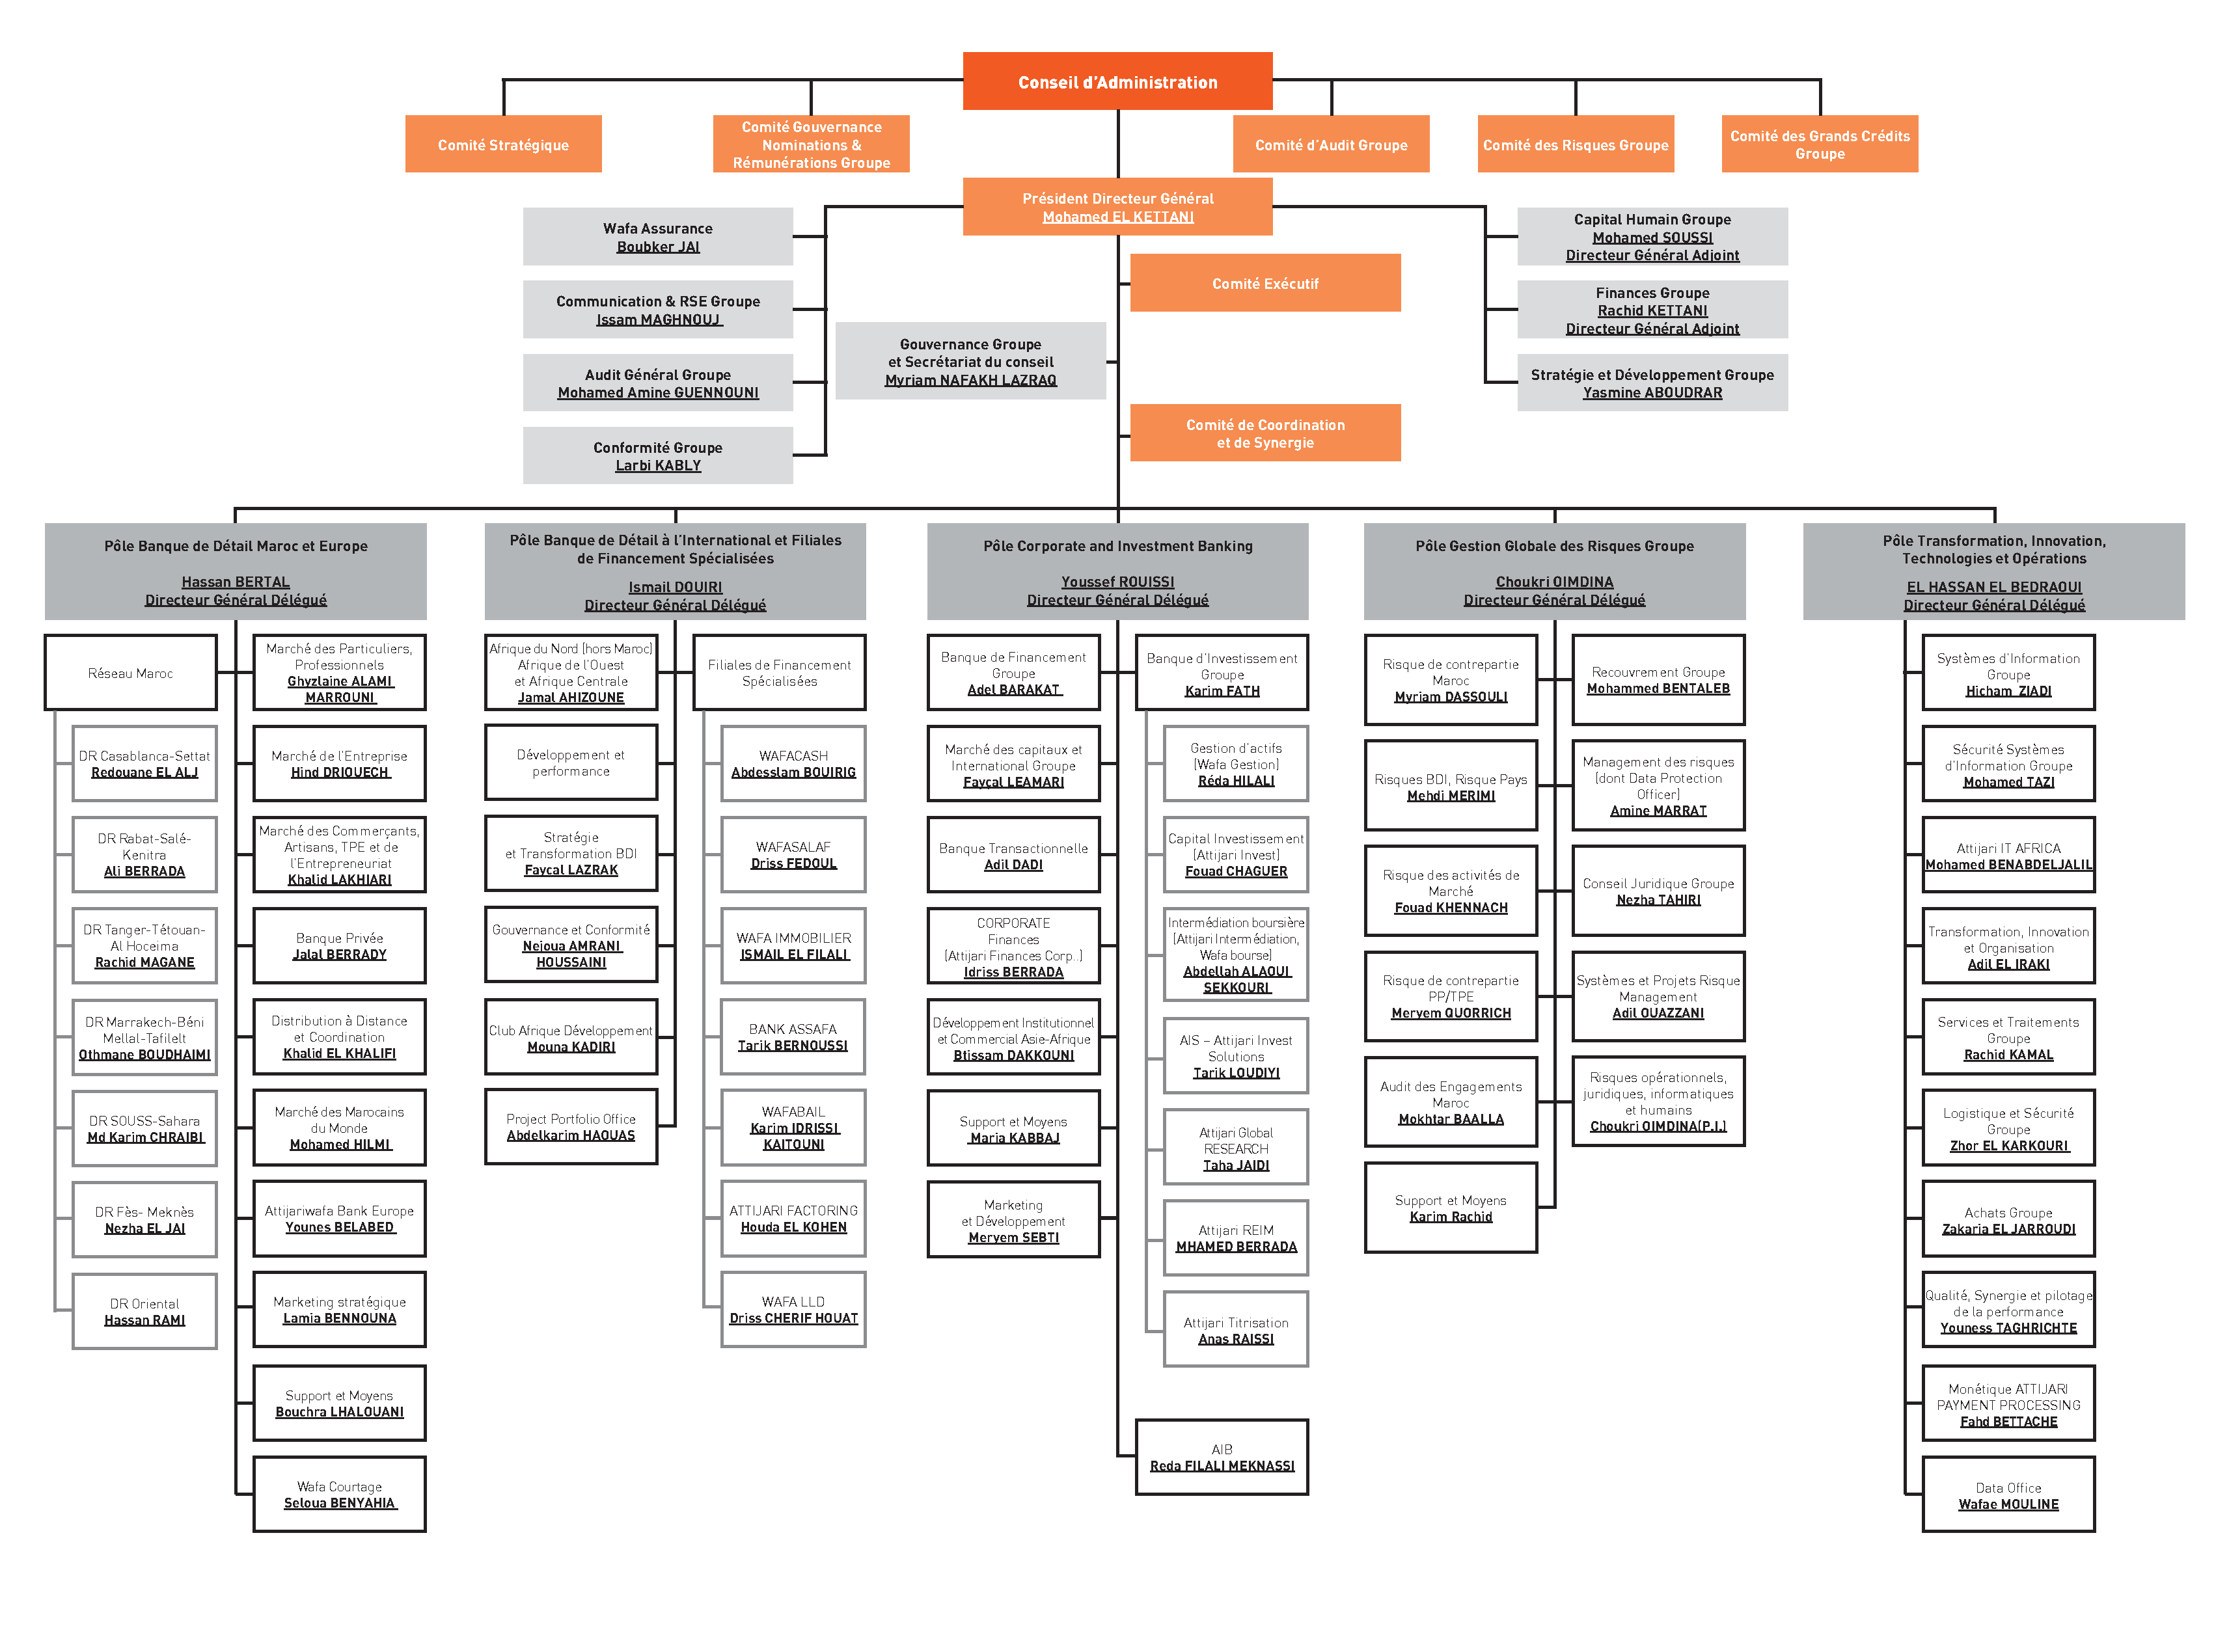
\includegraphics[width=1.1\textwidth]{organigramme.pdf}
    \caption{Organigramme AWB}
    \label{fig:organigramme}
\end{figure}

\FloatBarrier

\subsection{Cadrage du Projet}

Le projet a été initié dans un contexte où la banque souhaitait mieux exploiter ses données pour appuyer les décisions relatives au réseau d'agences. L'idée de départ était de proposer un outil lisible, concret et directement utile aux équipes métier, sans nécessiter d'expertise technique particulière pour son utilisation.

Le cadrage initial a permis de définir les attentes principales, d'identifier les données disponibles et de fixer les contraintes de réalisation. Il a aussi confirmé que le projet devait rester un outil d'aide à la décision : l'objectif n'est pas d'automatiser les choix stratégiques, mais de fournir une base d'analyse solide et compréhensible.

Les grandes orientations retenues dès le départ étaient les suivantes :
\begin{itemize}[leftmargin=1.2cm]
    \item analyser le réseau existant et identifier les agences performantes ou à risque ;
    \item détecter les zones de chevauchement entre agences proches ;
    \item repérer les zones géographiques sous-exploitées avec un potentiel de développement ;
    \item proposer une restitution visuelle et interactive des résultats ;
    \item rendre le tableau de bord accessible aux décideurs sans formation technique.
\end{itemize}

\section{Contexte du Projet}

Le secteur bancaire marocain traverse une période de transformation importante. La digitalisation des services, l'évolution des habitudes des clients et l'intensification de la concurrence poussent les banques à repenser leur présence physique. Les opérations courantes migrent vers les canaux numériques, mais les agences restent indispensables pour le conseil, la gestion de projets complexes et le maintien de la relation client.

Dans ce contexte, la question de la pertinence du réseau physique devient stratégique. Certaines agences sont très bien positionnées et génèrent des revenus élevés. D'autres se retrouvent trop proches de collègues ou mal positionnées par rapport au potentiel réel du quartier ou de la ville où elles sont implantées.

Ce projet propose une réponse concrète à ce besoin en construisant une plateforme capable de transformer des données brutes et dispersées en une information structurée, visuelle et utilisable pour la prise de décision.

\begin{figure}[htbp]
    \centering
    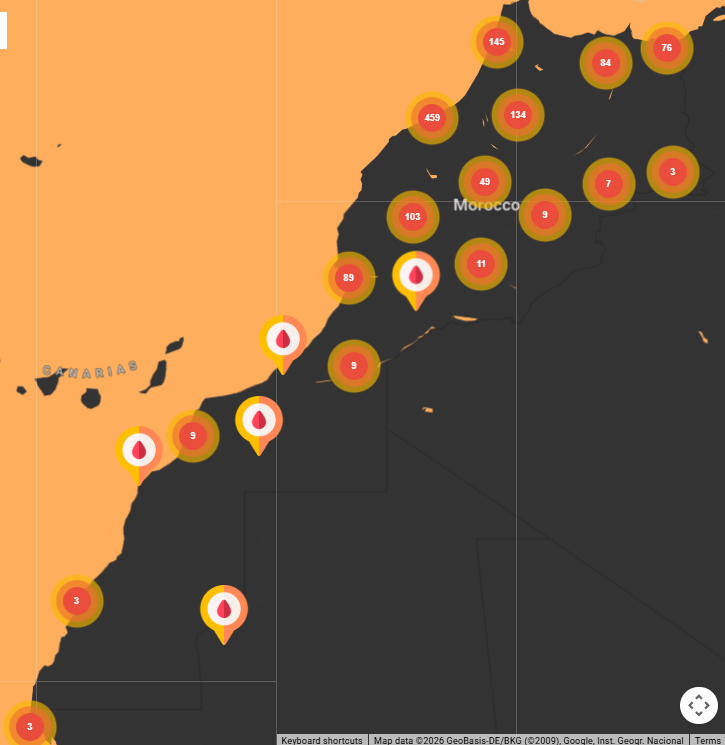
\includegraphics[width=0.5\textwidth]{reseauxawb.png}
    \caption{Reseaux AWB}
    \label{fig:reseaux}
\end{figure}

\FloatBarrier

\section{Problématique du Projet}

La problématique principale peut être formulée de la façon suivante :

\begin{quote}
\textit{Comment aider Attijariwafa Bank à analyser et optimiser son réseau d'agences à partir de la donnée géospatiale et des points d'intérêt, afin d'améliorer la prise de décision stratégique tout en maintenant une couverture territoriale cohérente sur l'ensemble du Maroc ?}
\end{quote}

Cette question centrale se décline en plusieurs points concrets :
\begin{itemize}[leftmargin=1.2cm]
    \item comment identifier les agences proches qui se font concurrence ou se cannibalisent mutuellement ;
    \item comment repérer les zones géographiques peu couvertes mais à fort potentiel commercial ;
    \item comment comparer objectivement des agences selon leur environnement immédiat ;
    \item comment présenter les résultats de manière simple, visuelle et exploitable sans expertise technique ;
    \item comment soutenir les décisions d'ouverture, de fermeture ou de fusion d'agences sur la base de données fiables.
\end{itemize}

Le projet n'a pas vocation à remplacer le jugement humain. Il fournit un support objectif et structuré qui permet aux responsables de prendre des décisions mieux informées et mieux documentées.


\section{Conduite du Projet}

Le projet a été conduit selon une approche progressive et itérative, ce qui est particulièrement adapté aux projets liés à la donnée. Cette façon de travailler permet de valider les résultats étape par étape et d'ajuster la direction en fonction des retours obtenus.

Les grandes phases du déroulement ont été les suivantes :
\begin{enumerate}[leftmargin=1.2cm]
    \item prise de connaissance du besoin métier et définition du périmètre ;
    \item exploration et analyse des données disponibles ;
    \item préparation et nettoyage des données ;
    \item développement du pipeline de scoring et de clustering ;
    \item développement de la sélection de nouveaux sites ;
    \item construction et validation du tableau de bord interactif.
\end{enumerate}

Chaque phase a fait l'objet d'une validation intermédiaire avant de passer à la suivante, ce qui a permis de garder une bonne maîtrise de l'avancement et de limiter les risques de dérives.

\section{Méthodologie de Travail}

Dans le cadre de mon projet de fin d'études portant sur l'optimisation du réseau d'agences
d'Attijariwafa Bank par une approche géospatiale et machine learning, j'ai adopté une
méthodologie de travail qui combine les principes de la méthode Agile avec les exigences
propres aux projets de data science.

\subsection{Choix de la méthode Agile}

L'adoption de la méthode Agile s'est imposée assez naturellement pour ce type de projet,
et ce pour plusieurs raisons :

\begin{itemize}[leftmargin=1.2cm]
    \item \textbf{Nature évolutive du projet :} Un projet d'analyse de données n'est pas figé
    dès le départ. Les résultats d'une étape orientent souvent ce qu'on fait dans la suivante,
    ce qui demande une méthode qui accepte les changements de direction.
    \item \textbf{Validation régulière :} Il était important de montrer des résultats concrets
    à l'encadrante et aux équipes concernées à intervalles réguliers, et non pas seulement
    à la toute fin du projet.
    \item \textbf{Gestion de l'incertitude :} Certaines étapes, comme la collecte des données
    ou la qualité des sources, n'étaient pas prévisibles à l'avance. La méthode Agile
    permet d'absorber ce genre d'imprévus sans remettre en cause tout le planning.
    \item \textbf{Avancement mesurable :} Travailler par petites étapes avec des livrables
    définis à chaque fois facilite le suivi et donne une vision claire de là où on en est.
\end{itemize}

\begin{figure}[htbp]
    \centering
    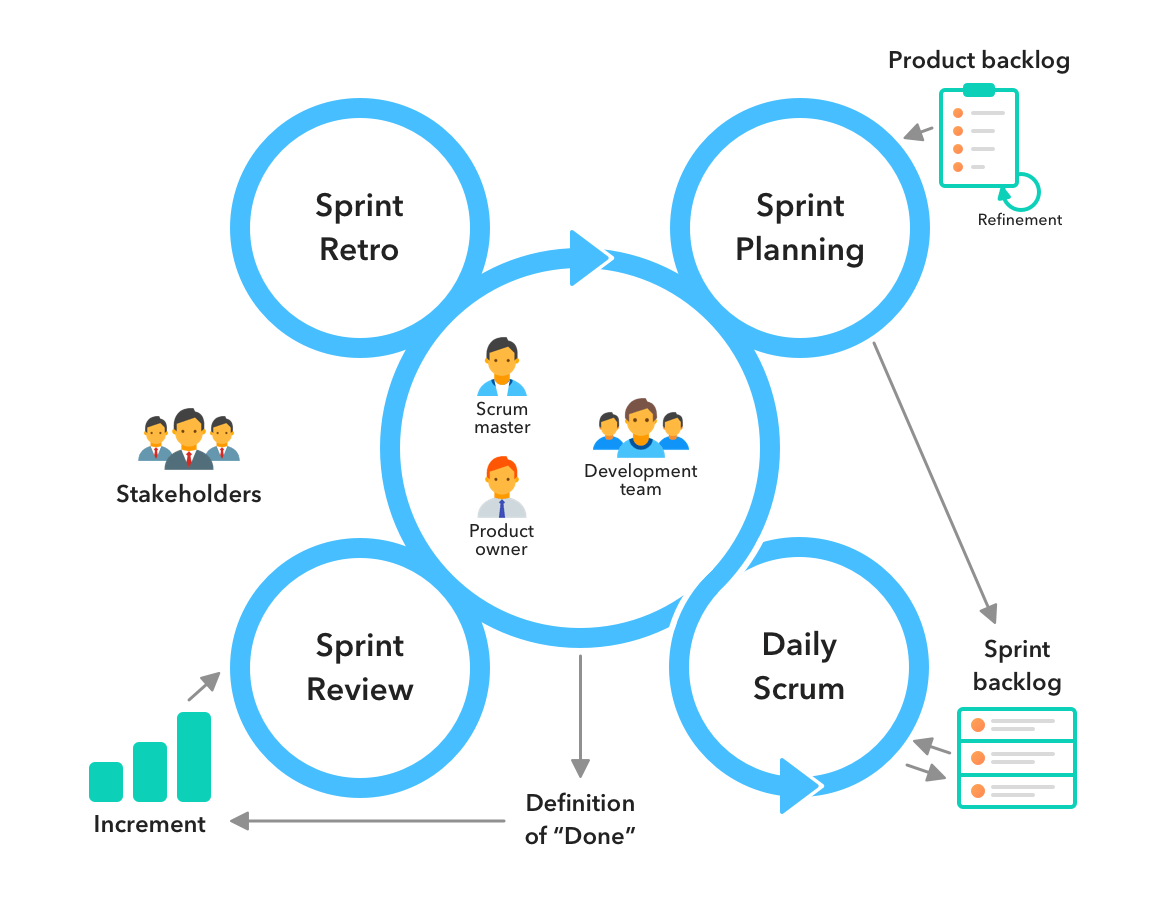
\includegraphics[width=0.65\textwidth]{scrum.png}
    \caption{Processus SCRUM et ses composants principaux}
    \label{fig:scrum}
\end{figure}

\subsection{Organisation des sprints}

Le projet a été découpé en sprints de deux semaines. Chacun avait un objectif précis
et un livrable attendu, ce qui permettait de valider le travail fait avant de passer
à la suite :

\begin{itemize}[leftmargin=1.2cm]
    \item \textbf{Planification du sprint :} En début de chaque sprint, on définissait les tâches
    à réaliser et les critères pour considérer que c'est terminé.
    \item \textbf{Points d'avancement réguliers :} Des échanges courts mais réguliers avec
    l'encadrante permettaient de signaler les blocages et de réajuster si nécessaire.
    \item \textbf{Revue de sprint :} À la fin de chaque sprint, les résultats étaient présentés
    et validés avant de lancer le suivant.
    \item \textbf{Rétrospective :} Un regard en arrière sur ce qui a bien fonctionné
    et ce qu'il fallait améliorer pour la prochaine itération.
\end{itemize}

\subsection{Adaptation aux spécificités du Data Science}

La méthode Agile a été ajustée pour tenir compte des particularités d'un projet
d'analyse de données :

\begin{itemize}[leftmargin=1.2cm]
    \item \textbf{Exploration avant développement :} Avant chaque sprint de production, une
    phase d'exploration rapide des données était faite pour s'assurer qu'on partait sur
    de bonnes bases.
    \item \textbf{Validation visuelle des résultats :} Chaque résultat intermédiaire était
    vérifié visuellement, par exemple sur une carte ou un graphique, pour s'assurer
    qu'il avait du sens avant d'aller plus loin.
    \item \textbf{Documentation au fil de l'eau :} Les choix techniques et les résultats
    étaient notés au fur et à mesure pour faciliter la rédaction du rapport et éviter
    de perdre des informations importantes.
    \item \textbf{Plans de secours :} Pour les étapes incertaines, notamment la collecte
    des données via des sources externes, des alternatives avaient été identifiées en amont.
\end{itemize}

\subsection{Outils et frameworks utilisés}

Pour mener à bien ce projet, plusieurs outils ont été utilisés selon les besoins
de chaque étape :

\begin{itemize}[leftmargin=1.2cm]
    \item \textbf{Python :} Langage principal utilisé pour tous les scripts de traitement,
    d'analyse et de modélisation.
    \item \textbf{Pandas et NumPy :} Pour la manipulation et le nettoyage des données.
    \item \textbf{Scikit-learn et SciPy :} Pour les algorithmes de clustering, de réduction
    de dimension et de calcul de similarité.
    \item \textbf{OpenStreetMap, Overture Maps et Google Maps :} Sources utilisées pour
    la collecte des points d'intérêt autour des agences.
    \item \textbf{Streamlit, Folium et Plotly :} Pour la construction du tableau de bord
    interactif et la visualisation des résultats sur carte.
    \item \textbf{Git :} Pour le suivi des versions du code tout au long du projet.
\end{itemize}

\subsection{Rôle et responsabilités}

En tant qu'étudiant stagiaire en charge du projet, j'ai assuré la totalité du
développement technique, depuis la collecte initiale des données jusqu'à la
livraison du tableau de bord final. Cela couvrait la conception des pipelines
de traitement, la mise en place des modèles d'analyse, les tests de validation
et la rédaction du présent rapport.

Les échanges réguliers avec mon encadrante académique,
et avec les équipes concernées au sein de la banque, ont permis de vérifier que
les choix faits correspondaient bien aux besoins réels du projet et aux attentes
des parties prenantes.

\subsection{Bénéfices observés}

Cette façon de travailler s'est avérée bien adaptée au projet. Parmi les points
positifs qu'on peut noter :

\begin{itemize}[leftmargin=1.2cm]
    \item \textbf{Détection rapide des problèmes :} Les anomalies dans les données ou les
    résultats inattendus ont été repérés tôt, ce qui a évité de les traîner jusqu'à la
    fin du projet.
    \item \textbf{Meilleure lisibilité de l'avancement :} Le découpage en sprints avec des
    livrables précis a rendu l'avancement du projet visible à tout moment.
    \item \textbf{Résultats concrets à chaque étape :} Plutôt que d'attendre la fin pour
    montrer quelque chose, chaque sprint produisait un résultat tangible qu'on pouvait
    présenter et discuter.
    \item \textbf{Apprentissage progressif :} Cette méthode a aussi permis de monter en
    compétence au fil du projet, en intégrant de nouvelles connaissances à chaque itération
    plutôt que d'essayer de tout apprendre d'un coup.
\end{itemize}

Cette approche s'est révélée particulièrement utile dans un environnement bancaire où
les données sont sensibles et où les résultats doivent être fiables et justifiables
avant d'être présentés aux décideurs.


\section{Planification du Projet}

La planification du projet a été formalisée sous forme d'un diagramme de Gantt, qui permet de visualiser l'enchaînement des tâches, leur durée et les éventuelles dépendances entre elles. Ce diagramme a servi de fil conducteur tout au long du stage pour s'assurer que le travail avançait dans les délais impartis.

\begin{figure}[H]
\centering
\begin{ganttchart}[
    hgrid,
    vgrid,
    x unit=0.55cm,
    y unit title=0.6cm,
    y unit chart=0.6cm,
    title height=1,
    bar height=0.6,
    group right shift=0,
    group top shift=0.7,
    group height=0.3,
    bar label node/.append style={align=left, anchor=east, text width=7.3cm},
    group label node/.append style={align=left, anchor=east, text width=7.3cm},
    bar label font=\small,
    title label font=\small\bfseries,
    milestone label font=\small\itshape,
    bar/.append style={fill=blue!50},
    bar incomplete/.append style={fill=blue!20},
    group/.append style={fill=black!70},
    milestone/.append style={fill=red, shape=diamond}
]{1}{20}
    % Titre des semaines
    \gantttitle{Semaines du stage (20 semaines)}{20} \\
    \gantttitlelist{1,...,20}{1} \\

    % Sprint 1 : Cadrage
    \ganttgroup{Sprint 1 : Cadrage et exploration}{1}{4} \\
    \ganttbar{Prise de connaissance du besoin}{1}{2} \\
    \ganttbar{Analyse exploratoire des données}{2}{4} \\

    % Sprint 2 : Collecte
    \ganttgroup{Sprint 2 : Collecte des données POI}{4}{9} \\
    \ganttbar{Extraction OSM et Overture Maps}{4}{5} \\
    \ganttbar{Scraping Google Maps}{5}{8} \\
    \ganttbar{Fusion et nettoyage des POI}{8}{9} \\

    % Sprint 3 : Scoring
    \ganttgroup{Sprint 3 : Pipeline de scoring}{9}{12} \\
    \ganttbar{Définition des catégories POI}{9}{10} \\
    \ganttbar{Calcul des scores normalisés}{10}{11} \\
    \ganttbar{Validation des résultats de scoring}{11}{12} \\

    % Sprint 4 : Clustering
    \ganttgroup{Sprint 4 : Clustering et analyse}{12}{15} \\
    \ganttbar{Application K-Means}{12}{13} \\
    \ganttbar{Analyse DBSCAN (zones denses)}{13}{14} \\
    \ganttbar{Visualisation PCA des clusters}{14}{15} \\

    % Sprint 5 : Sélection de sites
    \ganttgroup{Sprint 5 : Sélection de nouveaux sites}{15}{17} \\
    \ganttbar{Génération de la grille de candidats}{15}{16} \\
    \ganttbar{Similarité cosinus et scoring combiné}{16}{17} \\

    % Sprint 6 : Dashboard
    \ganttgroup{Sprint 6 : Tableau de bord}{16}{20} \\
    \ganttbar{Développement Streamlit / Folium}{16}{19} \\
    \ganttbar{Tests et validation utilisateur}{19}{20} \\

\end{ganttchart}
\caption{Diagramme de Gantt}
\end{figure}
\FloatBarrier

Le planning a été globalement respecté, avec quelques ajustements mineurs liés à la complexité de la collecte des données et au temps nécessaire pour valider la qualité des résultats intermédiaires. Le diagramme montre l'enchaînement logique des sprints et les deux jalons principaux : la livraison du pipeline de scoring à la dixième semaine et la livraison du tableau de bord à la dix-neuvième semaine.

%=============================================================================%
% CHAPITRE 2 : CONCEPTION FONCTIONNELLE
%=============================================================================%
\chapter{Conception Fonctionnelle}

Ce chapitre présente la conception fonctionnelle de la plateforme d'intelligence territoriale développée pour Attijariwafa Bank. Il décrit de manière détaillée le cahier des charges, les exigences fonctionnelles et non fonctionnelles, ainsi que la modélisation UML complète du système. Cette modélisation a été essentielle pour structurer le développement et garantir que la solution réponde aux besoins métier identifiés.

\section{Présentation du Cahier des Charges}

Le cahier des charges a été élaboré en collaboration avec les équipes métier d'Attijariwafa Bank et l'encadrante académique. Il définit les objectifs, le périmètre, les contraintes et les livrables attendus du projet.

\subsection{Contexte}

Attijariwafa Bank dispose d'un réseau de 1 196 agences réparties sur l'ensemble du territoire marocain. La gestion optimale de ce réseau constitue un enjeu stratégique majeur pour la banque, nécessitant des outils d'analyse capables d'évaluer la performance de chaque agence sur la base de son environnement géographique.

Dans cette optique, la plateforme a été conçue pour répondre à quatre besoins fondamentaux :

\begin{itemize}[leftmargin=1.2cm]
    \item \textbf{Évaluer} la performance de chaque agence sur la base de son environnement géographique ;
    \item \textbf{Identifier} les zones de redondance où plusieurs agences se cannibalisent mutuellement ;
    \item \textbf{Détecter} les zones sous-exploitées présentant un potentiel de développement ;
    \item \textbf{Proposer} des emplacements optimaux pour de nouvelles ouvertures basés sur des données objectives.
\end{itemize}

\subsection{Objectifs du Projet}

L'objectif principal de ce projet est de concevoir une plateforme d'aide à la décision offrant une vision complète du réseau d'agences et de ses opportunités d'expansion, tout en garantissant des standards élevés de performance, de fiabilité et d'utilisabilité. Le projet vise à accomplir les objectifs majeurs suivants :

\begin{enumerate}[leftmargin=1.2cm]
    \item \textbf{Valorisation des données territoriales :} Constituer une base de données riche en agrégeant des points d'intérêt géospatiaux, et assurer sa fiabilité via des mécanismes robustes de nettoyage et de validation des données.
    \item \textbf{Scoring multidimensionnel :} Calculer des indicateurs de performance reflétant l'attractivité de l'environnement de chaque agence (zones commerciales, résidentielles, concurrence, densité de population).
    \item \textbf{Profilage intelligent :} Regrouper les agences selon leurs caractéristiques géographiques pour identifier des profils de performance communs.
    \item \textbf{Sélection d'emplacements optimisée :} Recommander les meilleurs sites potentiels pour de nouvelles agences via des modèles prédictifs, tout en garantissant une optimisation algorithmique capable de traiter ces données géospatiales volumineuses dans des délais interactifs.
    \item \textbf{Visualisation et aide à la décision :} Offrir une interface analytique et cartographique intuitive permettant aux décideurs métier d'explorer les résultats et d'ajuster les paramètres sans nécessiter d'expertise technique.
    \item \textbf{Indépendance et maintenabilité :} Intégrer harmonieusement la solution dans l'écosystème d'Attijariwafa Bank en s'appuyant exclusivement sur des technologies open-source standardisées.
\end{enumerate}

\subsection{Périmètre du Système}

Le périmètre fonctionnel du système couvre l'ensemble du cycle de valorisation des données d'aide à la décision, structuré en trois volets principaux :

\begin{itemize}[leftmargin=1.2cm]
    \item \textbf{Les entrées :} L'intégration des données géographiques et financières des agences existantes, combinée à des données démographiques et à des points d'intérêt issus de sources cartographiques complémentaires.
    \item \textbf{Les traitements :} Le nettoyage et la consolidation des données, le calcul d'indicateurs d'attractivité territoriale, le profilage comportemental des agences (clustering), ainsi que l'évaluation prédictive et la sélection multicritère d'emplacements optimaux.
    \item \textbf{Les sorties :} La génération de recommandations d'optimisation du réseau (maintien, restructuration, fusion), la proposition de zones d'implantation à fort potentiel, et la mise à disposition de cartes interactives et de rapports exportables pour les décideurs.
\end{itemize}

\subsection{Livrables Attendus}

Le projet produit plusieurs livrables concrets, chacun couvrant une partie spécifique du pipeline de traitement.

Le \textbf{pipeline de scoring} des agences existantes, disponible dans le fichier \texttt{model/scoring.py}, calcule les sept scores multidimensionnels et les recommandations associées pour les 1 195 agences du réseau. Le \textbf{pipeline de sélection} de nouveaux sites, contenu dans \texttt{model2/site\_selection2.py}, identifie les vingt emplacements optimaux pour les nouvelles ouvertures en combinant un modèle de régression Random Forest entraîné dynamiquement, la similarité cosinus et le scoring POI. Un \textbf{notebook de benchmarking} (\texttt{model\_benchmarking.ipynb}) documente la comparaison rigoureuse entre quatre algorithmes de régression (Ridge, Random Forest, Gradient Boosting, XGBoost), démontrant la supériorité du Random Forest avec un $R^2$ de 0.88 en validation croisée à 5 plis. Le \textbf{tableau de bord interactif}, accessible dans \texttt{model2/dashboard.py}, offre neuf onglets couvrant l'ensemble des fonctionnalités de la plateforme, de la visualisation géographique à l'exécution interactive du modèle. Les \textbf{fichiers de résultats} incluent \texttt{branches\_scored.csv} pour les agences existantes et \texttt{site\_candidates\_full.csv} pour les sites potentiels. L'ensemble est complété par le présent rapport de stage et une documentation technique détaillée.

\section{Exigences Fonctionnelles}

Les exigences fonctionnelles décrivent ce que le système doit faire du point de vue de l'utilisateur. Elles ont été identifiées lors de la phase de cadrage et affinées au cours des sprints.

%-- Longtable: allows the table to break across pages naturally --%
\begingroup
\small
\renewcommand{\arraystretch}{1.1}
\rowcolors{1}{orange!15}{white}
\begin{longtable}{|p{3.5cm}|p{10.5cm}|}
\caption{Tableau des exigences fonctionnelles} \label{tab:ef} \\
\hline
\textbf{Fonctionnalité} & \textbf{Exigences Fonctionnelles} \\
\hline
\endfirsthead

\endhead
\hline
\endlastfoot

\textbf{Gestion des données POI} &
\begin{tblitem}
    \item Charger des fichiers POI provenant de trois sources (OSM, Google Maps, Overture Maps)
    \item Fusionner les fichiers et éliminer les doublons basés sur latitude/longitude
    \item Classer chaque POI dans une catégorie (commercial, bureau, résidentiel, transit, concurrent, agence propre)
    \item Produire un fichier merged\_data\_clean.csv consolidé
\end{tblitem} \\
\hline

\textbf{Scoring des agences existantes} &
\begin{tblitem}
    \item Calculer sept scores normalisés : commercial, bureaux, résidentiel, accessibilité, concurrence, cannibalisation, densité de population
    \item Calculer un score composite pondéré à partir des sept scores
    \item Attribuer une recommandation (KEEP, MONITOR, REVIEW, CLOSE) selon des seuils prédéfinis
    \item Regrouper les agences en 5 clusters via K-Means et étiqueter chaque cluster
    \item Produire un fichier branches\_scored.csv avec scores et recommandations
\end{tblitem} \\
\hline

\textbf{Sélection de nouveaux sites} &
\begin{tblitem}
    \item Générer une grille de points candidats avec espacement configurable (par défaut 0,7 km)
    \item Filtrer les points en mer ou zones inhabitées via validation de côte stricte
    \item Calculer un score POI par pondération inverse de la distance
    \item Identifier les 10\% meilleures agences par cluster comme référence
    \item Calculer la similarité cosinus entre chaque candidat et les agences benchmark
    \item Évaluer la densité de population via l'association à la ville la plus proche
    \item Calculer un score combiné paramétrable : $W_{\text{POI}} \times \text{POI} + W_{\text{SIM}} \times \text{similarité} + W_{\text{POP}} \times \text{densité de population}$
    \item Sélectionner le top 20 avec contraintes (max 2/ville, min 0,7 km entre sites)
    \item Entraîner dynamiquement un modèle Random Forest sur les agences existantes pour prédire le revenu mensuel en MAD de chaque site candidat
\end{tblitem} \\
\hline

\textbf{Visualisation et tableau de bord} &
\begin{tblitem}
    \item Afficher une carte interactive avec agences colorées selon leur recommandation
    \item Afficher les 20 sites recommandés avec marqueurs distinctifs
    \item Proposer des filtres par ville, action, cluster et score composite
    \item Afficher des graphiques (barres, camemberts, histogrammes, nuages de points)
    \item Permettre le téléchargement des résultats au format CSV
    \item Inclure un onglet d'exécution interactive avec upload et paramètres configurables
\end{tblitem} \\
\hline

\textbf{Exécution interactive du modèle} &
\begin{tblitem}
    \item Permettre l'upload de quatre fichiers CSV requis (incluant la densité de population)
    \item Permettre la configuration des paramètres (clusters, poids POI, poids population et poids similarité, espacement, contraintes)
    \item Afficher une barre de progression pendant l'exécution
    \item Afficher les résultats avec carte, graphiques et statistiques résumées
    \item Permettre le téléchargement (top 20 CSV, tous candidats CSV, métriques JSON)
\end{tblitem} \\
\hline

\textbf{Optimisation du réseau d'agences} &
\begin{tblitem}
    \item Entraîner dynamiquement un modèle d'évaluation financière
    \item Prédire le potentiel financier de chaque agence existante
    \item Calculer le ratio de performance (Revenu Réel / Revenu Prédit)
    \item Catégoriser les agences sur une matrice stratégique (Excellence, À surveiller, À revoir, À fermer)
    \item Détecter les opportunités de fusion géospatiale pour les agences peu performantes
    \item Afficher une matrice interactive et une carte de restructuration spatiale
    \item Permettre le téléchargement des résultats d'optimisation
\end{tblitem} \\

\end{longtable}
\endgroup

\subsection{Optimisation du Réseau (Matrice Stratégique)}

Dans un souci d'alignement avec les standards de l'industrie (tels que ceux prônés par les grands cabinets de conseil en stratégie), une fonctionnalité avancée d'\textbf{Optimisation du Réseau} a été intégrée. 

Ce pipeline repose sur trois piliers :
\begin{enumerate}[leftmargin=1.2cm]
    \item \textbf{Analyse des Écarts (Gap Analysis) :} Le système entraîne de manière dynamique un modèle prédictif pour estimer le revenu "attendu" d'une agence en fonction uniquement de son potentiel géographique (densité de population et attractivité locale). En comparant ce revenu attendu au revenu réel, le système calcule un "Ratio de Performance", permettant d'isoler le potentiel de l'emplacement de l'exécution managériale.
    \item \textbf{Matrice Stratégique BCG :} Les agences sont ensuite projetées sur une matrice interactive (Potentiel vs Exécution) et catégorisées automatiquement :
    \begin{itemize}[leftmargin=1cm]
        \item \textbf{FLAGSHIP} (Ratio $> 1.15$, Fort Potentiel) : Agences d'excellence.
        \item \textbf{REVIEW / INVEST} (Ratio $< 0.85$, Fort Potentiel) : Emplacement stratégique, mais sous-performance opérationnelle nécessitant un audit.
        \item \textbf{MONITOR} (Ratio $> 1.15$, Faible Potentiel) : Bonne exécution malgré une localisation limitante.
        \item \textbf{CLOSE} (Ratio $< 0.85$, Faible Potentiel) : Agences non rentables à fermer.
    \end{itemize}
    \item \textbf{Fusions Géospatiales Intelligentes :} Pour éviter la perte de parts de marché, le système utilise un algorithme de recherche spatiale de proximité. Pour chaque agence marquée comme \textit{CLOSE} ou \textit{REVIEW}, le système vérifie s'il existe une agence \textit{FLAGSHIP} dans un rayon d'action proche (environ 1,2 km). Si c'est le cas, la recommandation est intelligemment convertie en \textbf{MERGE} (Fusion), avec un traçage visuel sur la carte interactive.
\end{enumerate}

\section{Exigences Non Fonctionnelles}

Les exigences non fonctionnelles définissent les qualités que le système doit posséder, indépendamment de ses fonctionnalités.

\begingroup
\small
\renewcommand{\arraystretch}{1.1}
\rowcolors{1}{orange!15}{white}
\begin{longtable}{|p{3.2cm}|p{10.8cm}|}
\caption{Tableau des exigences non fonctionnelles} \label{tab:enf} \\
\hline
\textbf{Domaine} & \textbf{Exigences Techniques} \\
\hline
\endfirsthead
\endhead
\hline
\endfoot
\hline
\endlastfoot

\textbf{Performance} &
\begin{tblitem}
    \item Scoring des 1 195 agences en moins de 30 secondes
    \item Sélection de sites parmi 2 millions de points en moins de 5 minutes
    \item Chargement du dashboard et visualisations en moins de 10 secondes
    \item Exécution interactive du modèle en moins de 5 minutes
\end{tblitem} \\
\hline

\textbf{Fiabilité et Robustesse} &
\begin{tblitem}
    \item Gestion des données manquantes sans plantage (valeurs par défaut, imputation)
    \item Détection et suppression des doublons de POI
    \item Validation que les points candidats sont sur le territoire marocain
    \item Messages d'erreur clairs avec trace complète en cas d'échec
\end{tblitem} \\
\hline

\textbf{Utilisabilité} &
\begin{tblitem}
    \item Interface intuitive ne nécessitant aucune formation technique
    \item Visualisations claires, lisibles et informatives
    \item Paramètres configurables accompagnés de descriptions et valeurs par défaut
    \item Design professionnel cohérent avec l'image d'Attijariwafa Bank
\end{tblitem} \\
\hline

\textbf{Maintenabilité et Évolutivité} &
\begin{tblitem}
    \item Code modulaire et documenté pour faciliter les mises à jour
    \item Architecture permettant l'ajout facile de nouvelles sources de POI
    \item Algorithmes paramétrables pour s'adapter à différents contextes
    \item Support pour l'intégration future de données socio-économiques externes
\end{tblitem} \\
\hline

\textbf{Sécurité et Confidentialité} &
\begin{tblitem}
    \item Données traitées restant dans l'environnement sécurisé d'Attijariwafa Bank
    \item Aucune exposition de données sensibles en dehors du réseau interne
    \item Fichiers uploadés traités en mémoire sans persistance non contrôlée
\end{tblitem} \\

\end{longtable}
\endgroup

\section{Modélisation UML}

La modélisation UML (Unified Modeling Language) a été utilisée pour concevoir et documenter le système de manière visuelle et structurée. UML est un langage de modélisation standardisé qui permet de représenter les différentes facettes d'un système logiciel à l'aide de diagrammes.

\subsection{Choix d'UML pour la Modélisation}

Plusieurs raisons ont motivé le choix d'UML comme outil de modélisation pour ce projet. UML constitue un langage universellement reconnu dans l'industrie du logiciel, ce qui facilite grandement la communication entre les membres de l'équipe de développement et les différentes parties prenantes. Sa polyvalence offre une variété de diagrammes permettant de modéliser les différents aspects du système, qu'il s'agisse des aspects structurels comme les classes et les composants, ou des aspects comportementaux comme les cas d'utilisation et les séquences.

Dans le cadre spécifique de ce projet, nous avons principalement utilisé trois types de diagrammes :

\begin{itemize}[leftmargin=1.2cm]
    \item \textbf{Diagramme des cas d'utilisation :} Employé pour représenter les interactions entre les différents acteurs du système et les fonctionnalités offertes par la plateforme, permettant ainsi de visualiser qui fait quoi ;
    
    \item \textbf{Diagramme de séquence :} Utilisé pour détailler le déroulement temporel des traitements dans les pipelines de scoring et de sélection de sites, illustrant la chronologie précise des opérations et les échanges entre les composants ;
    
    \item \textbf{Diagramme d'activité :} Mobilisé pour illustrer le flux de données et les étapes successives de traitement ; ce diagramme est présenté en fin de chapitre et détaille notamment la nouvelle logique d'optimisation (Auto-ML).
\end{itemize}

La visualisation claire fournie par ces diagrammes complète la documentation textuelle et rend le système beaucoup plus compréhensible pour l'ensemble des intervenants, tout en facilitant la traçabilité des exigences jusqu'à leur implémentation technique concrète.

\section{Diagramme des Cas d'Utilisation}

Le diagramme des cas d'utilisation présente les interactions entre les acteurs du système et les fonctionnalités offertes par la plateforme.

\begin{figure}[htbp]
    \centering
    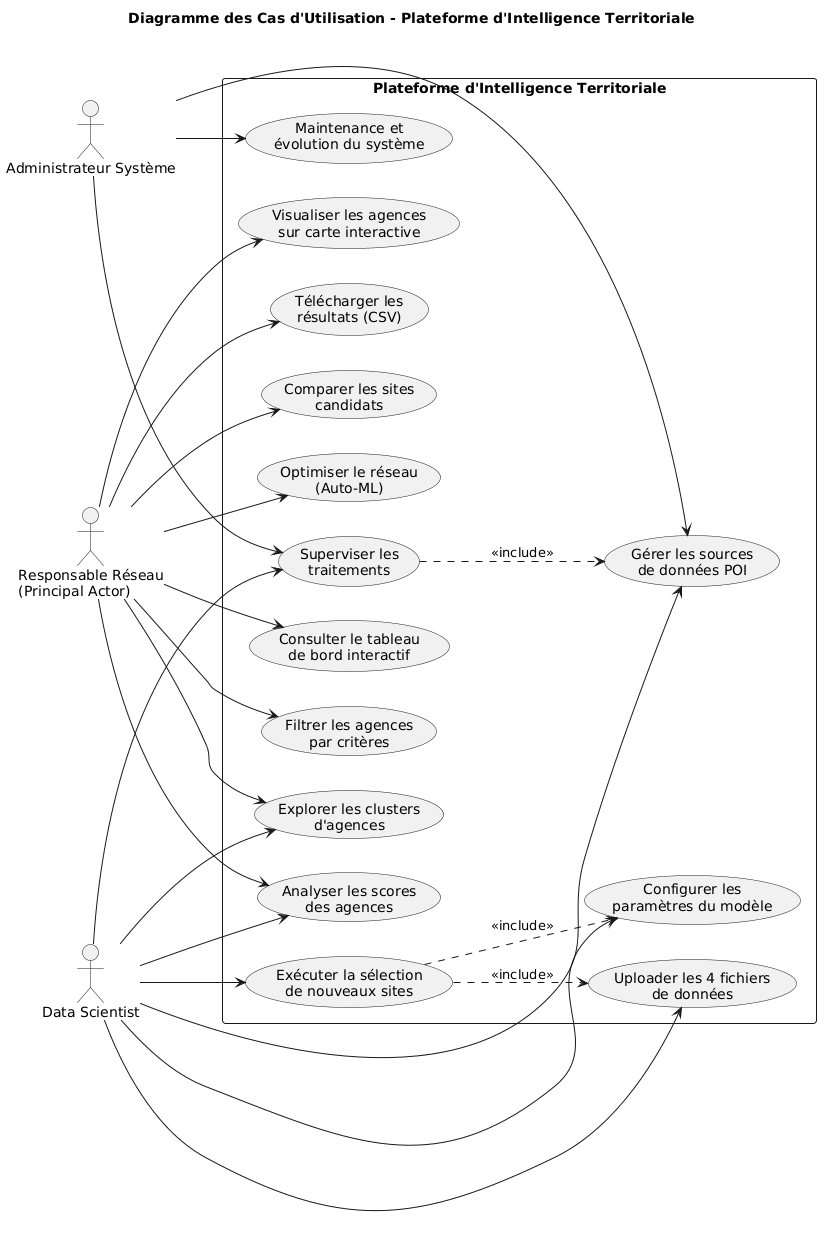
\includegraphics[width=0.80\textwidth]{use_case_diagram.png}
    \caption{Diagramme des cas d'utilisation}
    \label{fig:usecase}
\end{figure}

\FloatBarrier

\subsection{Description des Acteurs}

Le système comporte trois acteurs principaux aux rôles distincts et complémentaires, chacun intervenant à des niveaux différents du processus de prise de décision.

Le \textbf{Responsable Réseau} constitue l'utilisateur principal de la plateforme. Ses activités couvrent plusieurs aspects clés de l'analyse du réseau d'agences :

\begin{itemize}[leftmargin=1.2cm]
    \item Consultation du tableau de bord interactif pour une vue d'ensemble des performances ;
    \item Analyse détaillée des scores attribués à chaque agence et de leurs composantes ;
    \item Exploration des clusters formés par les agences similaires ;
    \item Visualisation des recommandations directement sur la carte géographique ;
    \item Téléchargement des résultats pour appuyer les décisions stratégiques d'expansion ou de restructuration.
\end{itemize}

Le \textbf{Data Scientist} endosse la responsabilité de l'exécution des modèles de sélection de nouveaux sites. Ses interventions portent sur :

\begin{itemize}[leftmargin=1.2cm]
    \item Configuration des paramètres algorithmiques (nombre de clusters, poids POI/population/similarité, espacement de la grille) ;
    \item Upload des fichiers de données sources requis pour l'exécution du modèle ;
    \item Supervision des traitements pour garantir la qualité et la fiabilité des résultats produits.
\end{itemize}

Enfin, l'\textbf{Administrateur Système} assure le bon fonctionnement global de la plateforme. Il est responsable de :

\begin{itemize}[leftmargin=1.2cm]
    \item La gestion des sources de données POI et le maintien des connexions aux différentes API ;
    \item La supervision de l'exécution des pipelines en surveillant les logs et les performances ;
    \item La maintenance évolutive du système et l'intégration de nouvelles fonctionnalités.
\end{itemize}

\subsection{Description des Cas d'Utilisation Principaux}

\begingroup
\small
\renewcommand{\arraystretch}{1.2}
\rowcolors{1}{orange!15}{white}
\begin{longtable}{|p{3.8cm}|p{9.7cm}|}
\caption{Description détaillée des cas d'utilisation} \label{tab:uc} \\
\hline
\textbf{Cas d'Utilisation} & \textbf{Description} \\
\hline
\endfirsthead
\endhead
\hline
\endfoot
\hline
\endlastfoot

UC1 : Consulter le tableau de bord interactif & L'utilisateur accède à la plateforme Streamlit qui affiche les KPIs globaux, les graphiques de performance et les visualisations des données \\
\hline
UC2 : Filtrer les agences par critères & L'utilisateur applique des filtres sur la ville, l'action recommandée, le cluster et le score composite pour affiner l'analyse \\
\hline
UC3 : Visualiser les agences sur carte interactive & L'utilisateur consulte la carte Folium avec les marqueurs colorés selon les recommandations et peut afficher les popups d'information \\
\hline
UC4 : Télécharger les résultats (CSV) & L'utilisateur exporte les données affichées (agences scorées, sites recommandés, métriques) au format CSV pour analyse externe \\
\hline
UC5 : Exécuter la sélection de nouveaux sites & L'utilisateur lance le pipeline complet de sélection de sites depuis le dashboard avec upload de fichiers et paramètres configurables \\
\hline
UC6 : Configurer les paramètres du modèle & L'utilisateur ajuste le nombre de clusters, les poids POI/population/similarité, l'espacement de grille et les contraintes de diversité géographique \\
\hline
UC7 : Uploader les fichiers de données & L'utilisateur charge les quatre fichiers CSV requis (branches\_scored.csv, branch\_performance.csv, merged\_data\_clean.csv, density.csv) \\
\hline
UC8 : Gérer les sources de données POI & L'administrateur configure et maintient les connexions aux sources OSM, Google Maps et Overture Maps pour la collecte des POI \\
\hline
UC9 : Superviser les traitements & L'administrateur surveille l'exécution des pipelines, vérifie les logs et intervient en cas d'erreur ou de performance dégradée \\
\hline
UC10 : Maintenance et évolution du système & L'administrateur met à jour le code, ajoute de nouvelles fonctionnalités et intègre de nouvelles sources de données \\
\hline
UC11 : Explorer les clusters d'agences & L'utilisateur analyse la répartition des agences en 5 clusters (High Performer, Commercial Hub, etc.) et visualise les caractéristiques de chaque groupe \\
\hline
UC12 : Analyser les scores des agences & L'utilisateur examine les sept scores normalisés et le score composite de chaque agence pour comprendre sa performance relative \\
\hline
UC13 : Comparer les sites candidats & L'utilisateur compare les sites recommandés selon le score combiné, le revenu prédit et la similarité aux meilleures agences \\
\hline
UC14 : Optimiser le réseau d'agences & L'utilisateur lance le pipeline d'évaluation des performances et de catégorisation stratégique des agences existantes \\
\hline
UC15 : Configurer les seuils d'analyse & L'utilisateur ajuste les ratios de sur-performance et sous-performance pour la matrice stratégique \\
\hline
UC16 : Consulter la matrice stratégique & L'utilisateur analyse le positionnement des agences selon leur potentiel géographique et leur exécution managériale \\
\hline
UC17 : Visualiser les recommandations & L'utilisateur explore la carte des restructurations suggérées incluant les fermetures et fusions \\
\hline
UC18 : Télécharger les données d'optimisation & L'utilisateur exporte les ratios de performance et recommandations stratégiques au format CSV \\

\end{longtable}
\endgroup

\section{Diagramme de Séquence}

Le diagramme de séquence détaille l'ordre temporel des interactions entre l'utilisateur, le tableau de bord (dashboard) et les pipelines de traitement lors de l'exécution de la sélection de nouveaux sites, qui est la fonctionnalité la plus complexe du système.

\begin{figure}[htbp]
    \centering
    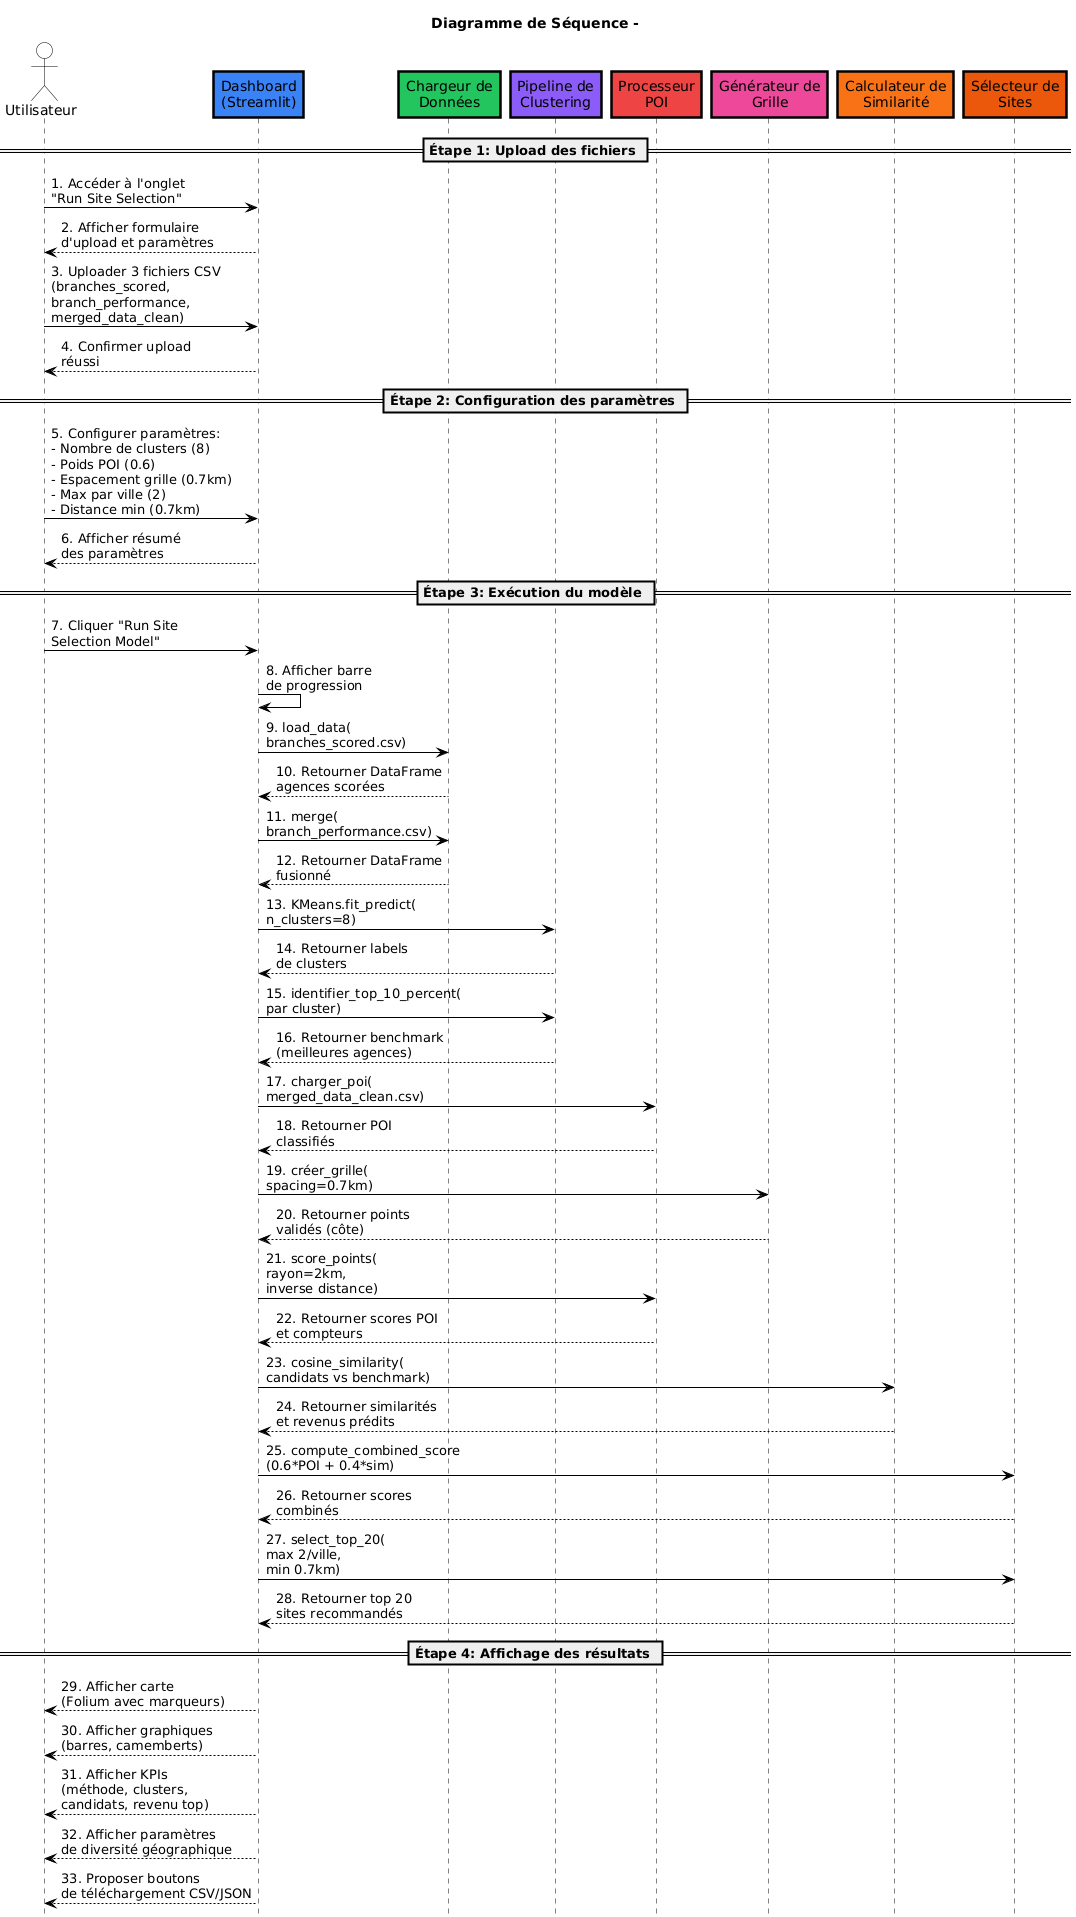
\includegraphics[width=0.80\textwidth]{sequence_diagram.png}
    \caption{Diagramme de séquence}
    \label{fig:sequence}
\end{figure}

\FloatBarrier

\subsection{Description Détaillée des Étapes}

Le diagramme de séquence présenté ci-dessus illustre le workflow complet de l'exécution de la sélection de nouveaux sites, depuis l'initialisation par l'utilisateur jusqu'à l'affichage des résultats finaux. Ce processus se décompose en six phases successives, chacune jouant un rôle essentiel dans la chaîne de traitement.

\subsubsection*{Phase 1 : Initialisation}

Cette première phase correspond aux premiers échanges entre l'utilisateur et le système. L'utilisateur navigue vers l'onglet dédié à la sélection de sites au sein du tableau de bord, où le système affiche le formulaire d'upload avec les quatre champs requis pour les fichiers de données (données existantes, performances, POIs et densités par ville) ainsi que les paramètres configurables disponibles. L'utilisateur procède alors au téléchargement des fichiers CSV nécessaires, et le système valide la conformité de ces fichiers avant de confirmer le succès de l'opération.

\subsubsection*{Phase 2 : Configuration des Paramètres}

Cette phase voit l'utilisateur ajuster les différents paramètres du modèle à l'aide des curseurs et cases à cocher mis à sa disposition dans l'interface. Les paramètres configurables incluent :

\begin{itemize}[leftmargin=1.2cm]
    \item Le \textbf{nombre de clusters} pour l'algorithme K-Means (par défaut 8) ;
    \item Les \textbf{poids relatifs} attribués au score POI et à la densité de population dans le calcul combiné (le poids de la similarité se déduisant de ceux-ci) ;
    \item L'\textbf{espacement} entre les points de la grille de candidats (par défaut 0,7 km) ;
    \item Les \textbf{contraintes de diversité géographique} limitant le nombre d'agences par ville et la distance minimale entre sites sélectionnés.
\end{itemize}

Le système affiche ensuite un résumé synthétique de l'ensemble des paramètres pour validation finale avant l'exécution, permettant de personnaliser l'exécution selon les besoins stratégiques du moment.

\subsubsection*{Phase 3 : Traitement Initial des Données}

Le tableau de bord charge les données des agences existantes puis les fusionne avec les données de performance financière en utilisant le nom de l'agence comme clé de jointure. La densité de population est ensuite rattachée à chaque agence via une recherche de proximité géographique, identifiant pour chaque agence la ville la plus proche. Le système de segmentation applique ensuite un algorithme de partitionnement pour classer les agences en différents profils. Une fois cette segmentation terminée, les meilleures agences de chaque profil sont identifiées en se basant sur leur revenu pour former le jeu de référence (benchmark). Ces agences d'excellence serviront de profil idéal que les nouveaux sites candidats devront approcher.

\subsubsection*{Phase 4 : Traitement des Points d'Intérêt et Génération de la Grille}

Cette phase concerne le traitement de l'environnement local et la création de la grille de candidats potentiels. Le système procède à la classification de chaque point d'intérêt dans l'une des six catégories définies (commercial, bureau, résidentiel, transit, concurrent ou propre réseau). Parallèlement, un maillage crée des points candidats couvrant l'intégralité du territoire selon l'espacement configuré par l'utilisateur.

Plusieurs filtres sont ensuite appliqués pour garantir la pertinence des candidats :

\begin{itemize}[leftmargin=1.2cm]
    \item \textbf{Validation géographique :} Élimination des points situés en mer ou dans des zones inhabitées ;
    \item \textbf{Filtrage de proximité :} Écartement des points trop proches d'une agence existante pour éviter les redondances ;
    \item \textbf{Filtrage par attractivité :} Suppression des candidats avec un environnement immédiat trop pauvre en activité.
\end{itemize}

Le système évalue enfin un score d'attractivité pour chaque point candidat survivant en utilisant une pondération inversement proportionnelle à la distance. À cette étape, la métrique de densité de population est également récupérée pour chaque candidat en identifiant la zone urbaine la plus proche, puis normalisée sur l'ensemble de la grille.

\subsubsection*{Phase 5 : Prédiction, Similarité et Sélection Finale}

Cette phase constitue le cœur algorithmique du processus et se décompose en deux étapes distinctes.

Dans un premier temps, le système entraîne dynamiquement un modèle d'apprentissage supervisé prédictif sur les données des agences existantes. Les caractéristiques d'entraînement sont les scores d'attractivité territoriale et la densité de population, la variable cible étant le revenu mensuel. Les valeurs aberrantes sont exclues et les données sont standardisées mathématiquement. Ce modèle, sélectionné pour sa robustesse lors d'une phase préalable de validation croisée, est ensuite appliqué à l'ensemble des candidats de la grille pour produire la prédiction de revenu financier de chaque site.

Dans un second temps, le calculateur détermine la similarité mathématique (mesure cosinus) entre le profil de chaque candidat et les profils des agences de référence identifiées précédemment. Cette métrique de similarité sert de composante d'ajustement.

Le sélecteur calcule ensuite le score combiné paramétrable selon la formule :

\begin{center}
\textbf{Score Combiné} = $W_{\text{POI}} \times \text{Score POI} + W_{\text{SIM}} \times \text{Similarity} + W_{\text{POP}} \times \text{Score Densité Population}$
\end{center}

Puis procède à la sélection du top 20 des emplacements en appliquant rigoureusement les contraintes de diversité géographique configurées précédemment, à savoir un maximum de deux agences par ville et une distance minimale de sept cents mètres entre chaque site sélectionné.

\subsubsection*{Phase 6 : Visualisation des Résultats}

La dernière phase correspond à l'affichage structuré de l'ensemble des résultats obtenus. Le tableau de bord présente plusieurs éléments clés :

\begin{itemize}[leftmargin=1.2cm]
    \item \textbf{Carte interactive :} Les vingt sites recommandés sous forme de marqueurs, superposés aux agences existantes du réseau ;
    \item \textbf{Graphiques analytiques :} Visualisations des revenus prédits, des scores de similarité, de la distribution territoriale et de la répartition financière ;
    \item \textbf{Indicateurs de performance :} Résumé de la méthode employée, de la volumétrie traitée et des potentiels maximaux identifiés ;
    \item \textbf{Fonctionnalités d'export :} Téléchargement des résultats sous formats structurés pour permettre leur intégration dans d'autres outils décisionnels.
\end{itemize}



\section{Diagramme de Séquence : Optimisation du Réseau}

Ce troisième diagramme de séquence illustre le fonctionnement du module d'optimisation du réseau. Ce processus permet d'évaluer la performance d'exécution des agences en la séparant de la qualité de leur emplacement géographique.

\begin{figure}[htbp]
    \centering
    \includegraphics[width=0.80\textwidth]{sequence_diagram_network_opt.png}
    \caption{Diagramme de séquence de l'optimisation du réseau}
    \label{fig:seq_opt}
\end{figure}

\FloatBarrier

\subsection{Description Détaillée des Étapes}

L'exécution se décompose en quatre phases principales :

\subsubsection*{Phase 1 : Configuration Initiale}
L'utilisateur accède à l'onglet d'optimisation du réseau et configure les seuils d'analyse. Ces seuils définissent à partir de quel écart un ratio est considéré comme de la sur-performance ou de la sous-performance.

\subsubsection*{Phase 2 : Modélisation et Évaluation}
Au lancement de l'optimisation, le système fusionne les données des agences avec leurs données de performances financières. Un modèle d'évaluation est entraîné afin d'apprendre la relation entre l'attractivité territoriale et le revenu. Le modèle prédit ensuite le revenu attendu pour chaque agence, permettant au système de calculer un ratio de performance (revenu réel divisé par revenu attendu).

\subsubsection*{Phase 3 : Catégorisation Stratégique}
Sur la base de ce ratio, l'analyseur stratégique classe les agences en plusieurs catégories d'action. Ensuite, une recherche spatiale est effectuée pour les agences à faible performance afin de vérifier si une agence d'excellence se trouve à proximité, transformant ainsi une recommandation de fermeture simple en une recommandation de fusion stratégique.

\subsubsection*{Phase 4 : Restitution et Export}
Les résultats sont finalement présentés à l'utilisateur sous la forme d'une matrice stratégique interactive et d'une carte géographique illustrant les restructurations proposées. L'utilisateur peut télécharger ces recommandations pour la planification opérationnelle.

\section{Diagramme d'Activité}

Le diagramme d'activité illustre le flux de données global de la plateforme, depuis l'ingestion des sources hétérogènes (POI, performances financières, démographie) jusqu'à la sélection finale de nouveaux sites et la restitution sur le tableau de bord. Il met particulièrement en évidence la logique d'optimisation du réseau impliquant l'entraînement d'un modèle d'évaluation, le calcul du ratio de performance et l'application des règles spatiales de proximité pour détecter les opportunités de fusion.

\begin{figure}[htbp]
    \centering
    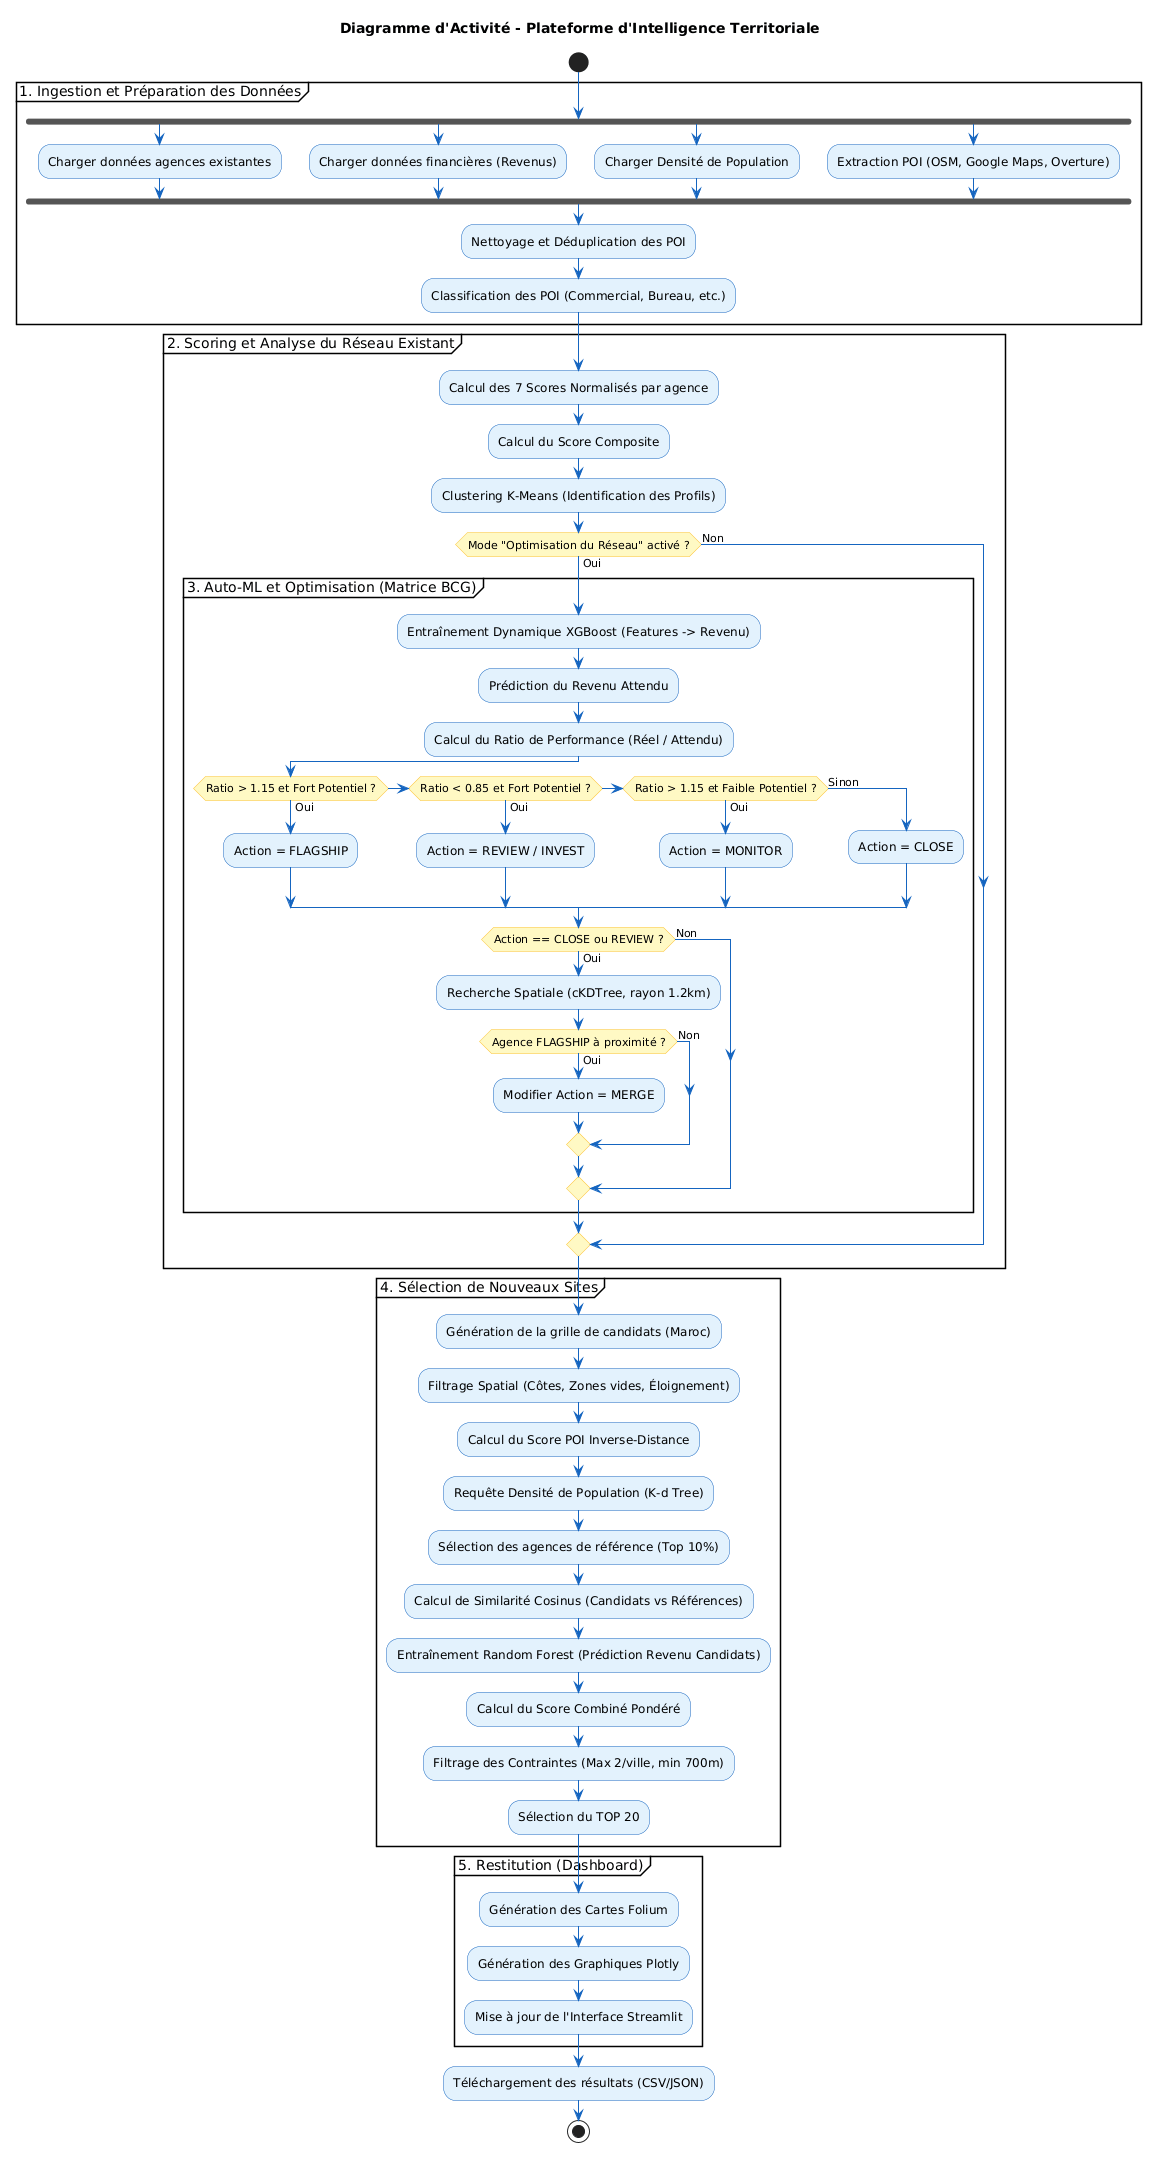
\includegraphics[width=0.80\textwidth]{activity_diagram.png}
    \caption{Diagramme d'activité de la plateforme}
    \label{fig:activity}
\end{figure}

\FloatBarrier




%=============================================================================%
% CHAPITRE 3 : CADRE THÉORIQUE ET FONDEMENTS MATHÉMATIQUES
%=============================================================================%
\chapter{Cadre Théorique et Fondements Mathématiques}

Ce chapitre constitue le socle théorique de l'ensemble du projet. L'ingénierie des données et la modélisation prédictive exigent une compréhension rigoureuse des mécanismes mathématiques sous-jacents aux algorithmes employés. Ainsi, ce chapitre dépasse la simple abstraction algorithmique pour plonger au cœur de l'optimisation, du calcul différentiel, de l'algèbre linéaire et de la théorie probabiliste qui régissent les modèles d'apprentissage automatique utilisés pour la sélection de sites et l'optimisation du réseau.

%-----------------------------------------------------------------------------%
\section{Fondements Théoriques de l'Apprentissage Automatique}
%-----------------------------------------------------------------------------%

L'apprentissage automatique (Machine Learning) repose sur la capacité d'un système à inférer des règles mathématiques complexes à partir de données empiriques $\mathcal{D}$, dans le but de généraliser ces règles à de nouvelles instances invisibles \cite{mitchell1997}.

\subsection{Paradigmes d'Apprentissage}

Les algorithmes mobilisés dans ce projet s'inscrivent dans deux paradigmes distincts mais complémentaires :

\begin{itemize}[leftmargin=1.2cm]
    \item \textbf{L'apprentissage non supervisé :} Dans ce cadre, l'ensemble de données $\mathcal{D} = \{x_1, x_2, \dots, x_N\}$ est dépourvu d'étiquettes. L'objectif est d'identifier la topologie sous-jacente ou la structure latente de l'espace des caractéristiques $\mathbb{R}^d$. Nous mobilisons ces algorithmes (K-Means, DBSCAN, PCA) pour segmenter le réseau existant, identifier les zones géographiques denses, et réduire la dimensionnalité de l'espace de représentation.
    \item \textbf{L'apprentissage supervisé :} L'ensemble de données est constitué de paires $\mathcal{D} = \{(x_1, y_1), \dots, (x_N, y_N)\}$ où $x_i \in \mathbb{R}^d$ est le vecteur de caractéristiques (les scores POI, la densité) et $y_i \in \mathbb{R}$ est la cible continue (le revenu financier). L'algorithme cherche à approximer une fonction inconnue $F: \mathbb{R}^d \rightarrow \mathbb{R}$ minimisant l'espérance mathématique d'une fonction de perte.
\end{itemize}

\subsection{Le Compromis Biais-Variance}

L'un des défis fondamentaux de la modélisation prédictive est le compromis Biais-Variance (Bias-Variance Tradeoff) \cite{hastie2009}. L'erreur de généralisation attendue $\text{Err}(x)$ d'un modèle $\hat{f}(x)$ pour un point $x$ donné, face à un véritable signal $f(x)$ bruité par $\epsilon \sim \mathcal{N}(0, \sigma^2)$, se décompose mathématiquement ainsi :

\begin{equation}
\text{Err}(x) = \mathbb{E}\left[ (y - \hat{f}(x))^2 \right]
\end{equation}

En développant cette espérance, le théorème de décomposition prouve que :
\begin{equation}
\text{Err}(x) = \left( \mathbb{E}[\hat{f}(x)] - f(x) \right)^2 + \mathbb{E}\left[ (\hat{f}(x) - \mathbb{E}[\hat{f}(x)])^2 \right] + \sigma^2
\end{equation}

Ce qui se traduit par :
\begin{equation}
\text{Err}(x) = \text{Biais}(\hat{f}(x))^2 + \text{Var}(\hat{f}(x)) + \text{Bruit Irréductible}
\end{equation}

\begin{itemize}
    \item Le \textbf{Biais} quantifie l'erreur due à des hypothèses simplistes du modèle (ex: régression linéaire sur des données non linéaires), conduisant au sous-apprentissage (Underfitting).
    \item La \textbf{Variance} quantifie la sensibilité du modèle aux fluctuations de l'ensemble d'entraînement. Un modèle à forte variance modélise le bruit géospatial aléatoire, conduisant au surapprentissage (Overfitting).
\end{itemize}

Tout l'enjeu du paramétrage des modèles (comme la profondeur des arbres XGBoost) consiste à trouver le point d'inflexion minimisant la somme de ces deux erreurs.

\subsection{Surapprentissage et Validation Croisée (K-Fold)}

Pour estimer de manière non biaisée l'erreur de généralisation et éviter le surapprentissage, la méthode de la validation croisée à K-plis (K-Fold Cross-Validation) est une norme académique stricte. 

L'ensemble de données $\mathcal{D}$ est partitionné aléatoirement en $K$ sous-ensembles mutuellement exclusifs $D_1, D_2, \dots, D_K$ de tailles approximativement égales. Le modèle est entraîné sur $K-1$ sous-ensembles et évalué sur le sous-ensemble restant $D_k$. Ce processus est itéré $K$ fois. L'erreur estimée par validation croisée, $CV_{(K)}$, est la moyenne arithmétique des erreurs de chaque pli :

\begin{equation}
CV_{(K)} = \frac{1}{K} \sum_{k=1}^{K} L_k(y, \hat{f}^{-k}(x))
\end{equation}
où $\hat{f}^{-k}$ est le modèle entraîné sans le sous-ensemble $k$. Dans notre modélisation financière, l'utilisation systématique de cette méthode garantit que nos prédictions de revenus pour de nouvelles agences ne souffrent pas de mémorisation des données d'entraînement.

%-----------------------------------------------------------------------------%
\section{Théorie du Prétraitement et Qualité des Données}
%-----------------------------------------------------------------------------%

La robustesse des algorithmes spatiaux dépend intrinsèquement de la distribution statistique des données en entrée. Le prétraitement n'est donc pas une étape heuristique, mais repose sur des transformations mathématiques strictes.

\subsection{Standardisation Statistique (Z-Score)}

La standardisation est impérative lorsque les caractéristiques n'évoluent pas dans les mêmes échelles de grandeur (par exemple, la distance en mètres vs le nombre de banques concurrentes). L'absence de standardisation perturbe sévèrement les fonctions de distance Euclidienne (utilisées par K-Means et cKDTree) et ralentit la convergence des algorithmes basés sur la descente de gradient.

La transformation Z-score centre la distribution autour de zéro et réduit son écart-type à l'unité. Pour une variable aléatoire $X_j$ d'espérance $\mu_j$ et d'écart-type $\sigma_j$, la variable standardisée $Z_j$ est définie par :

\begin{equation}
Z_{ij} = \frac{x_{ij} - \mu_j}{\sigma_j}
\end{equation}

Ainsi, $\mathbb{E}[Z_j] = 0$ et $\text{Var}(Z_j) = 1$. Cette transformation isométrique préserve la corrélation entre les variables tout en stabilisant le conditionnement des matrices lors de l'apprentissage.

\subsection{Traitement Statistique des Valeurs Aberrantes (Outliers)}

Les valeurs aberrantes financières (agences générant des revenus statistiquement anormaux) déforment la fonction de perte $L_2$, qui pénalise ces écarts quadratiquement. Pour identifier ces valeurs de manière robuste (c'est-à-dire sans être influencé par la moyenne qui est elle-même sensible aux extrêmes), la méthode de l'Écart Interquartile (Interquartile Range - IQR) est privilégiée.

Soient $Q_1$ et $Q_3$ les premier et troisième quartiles de la distribution des revenus $Y$. L'IQR est défini comme la dispersion de la moitié centrale des données :
\begin{equation}
\text{IQR} = Q_3 - Q_1
\end{equation}

Une observation $y_i$ est considérée comme aberrante si elle n'appartient pas à l'intervalle de confiance défini par le paramètre de sévérité $\tau$ (généralement $\tau=1.5$) :
\begin{equation}
y_i \notin \left[ Q_1 - \tau \cdot \text{IQR}, \quad Q_3 + \tau \cdot \text{IQR} \right]
\end{equation}
Les observations en dehors de ces bornes (Tukey's fences) sont soit écrêtées (Clipping/Winsorisation) soit exclues pour préserver la stabilité asymptotique du modèle de régression.

%-----------------------------------------------------------------------------%
\section{Apprentissage Non Supervisé et Modélisation Géospatiale}
%-----------------------------------------------------------------------------%

\subsection{K-Means et Optimisation de Lloyd}

L'algorithme K-Means \cite{macqueen1967} cherche à partitionner l'espace $\mathbb{R}^d$ en $K$ sous-ensembles $S = \{S_1, S_2, \dots, S_K\}$ en minimisant la variance intra-cluster (Inertie). Mathématiquement, il s'agit de la résolution d'un problème d'optimisation non convexe :

\begin{equation}
\arg\min_{S} \sum_{k=1}^{K} \sum_{x_i \in S_k} || x_i - \mu_k ||^2_2
\end{equation}

où $\mu_k$ est le centroïde du cluster $S_k$. L'algorithme de Lloyd résout ce problème de manière itérative. La démonstration stipulant que le centroïde optimal est strictement la moyenne arithmétique s'obtient en annulant le gradient de la fonction de coût $J$ par rapport à $\mu_k$ :

\begin{equation}
\nabla_{\mu_k} J = \nabla_{\mu_k} \sum_{x_i \in S_k} (x_i - \mu_k)^T (x_i - \mu_k) = -2 \sum_{x_i \in S_k} (x_i - \mu_k) = 0
\end{equation}

En isolant $\mu_k$, nous obtenons l'équation de mise à jour formelle :
\begin{equation}
\mu_k = \frac{1}{|S_k|} \sum_{x_i \in S_k} x_i
\end{equation}

\subsection{Initialisation Probabiliste : K-Means++}

L'algorithme de Lloyd est sensible à l'initialisation des centroïdes et peut converger vers des minimums locaux sous-optimaux. Pour y remédier, l'algorithme K-Means++ (Arthur et Vassilvitskii, 2007) propose une initialisation probabiliste. Le premier centroïde $c_1$ est choisi uniformément au hasard parmi les points de données. Ensuite, pour chaque point $x_i$, on calcule la distance $D(x_i)$ par rapport au centroïde le plus proche déjà choisi. Le prochain centroïde est tiré avec une probabilité proportionnelle au carré de cette distance :

\begin{equation}
P(x_i = c_{nouveau}) = \frac{D(x_i)^2}{\sum_{j=1}^{N} D(x_j)^2}
\end{equation}

Cette approche écarte algorithmiquement les centroïdes initiaux, garantissant une approximation en espérance de l'ordre de $O(\log K)$ du minimum global de l'inertie.

\subsection{Évaluation du Clustering : Le Score de Silhouette}

Puisque nous ne disposons pas de vérité terrain (Ground Truth) pour valider la segmentation des agences, des métriques de validation interne doivent être appliquées. Le Coefficient de Silhouette évalue simultanément la compacité d'un cluster et sa séparation vis-à-vis des autres.

Pour une observation $i \in S_k$, on définit :
- $a(i)$ : la distance moyenne intra-cluster (cohésion).
- $b(i)$ : la distance moyenne au cluster le plus proche $S_m$ avec $m \neq k$ (séparation).

Le score de silhouette $s(i)$ pour le point $i$ s'écrit :
\begin{equation}
s(i) = \frac{b(i) - a(i)}{\max\{a(i), b(i)\}}
\end{equation}

Le score global est l'espérance $\mathbb{E}[s(i)]$ sur l'ensemble du jeu de données. Encadré dans $[-1, 1]$, un score proche de $1$ indique une segmentation de haute qualité, tandis qu'un score négatif indique des assignations incorrectes.

\subsection{Clustering Basé sur la Densité : DBSCAN}

Alors que K-Means contraint les clusters à une forme hypersphérique (Voronoï), l'algorithme DBSCAN (Density-Based Spatial Clustering of Applications with Noise) \cite{ester1996} identifie des régions de haute densité spatiale de forme arbitraire. Cette méthode est cruciale dans la modélisation urbaine pour distinguer les zones très denses des zones éparses.

DBSCAN repose sur deux hyperparamètres : un rayon $\epsilon$ et un nombre minimum de points $MinPts$. Le concept clé est l'$\epsilon$-voisinage d'un point $p$, noté $N_\epsilon(p)$ :
\begin{equation}
N_\epsilon(p) = \{q \in \mathcal{D} \mid ||p - q||_2 \le \epsilon\}
\end{equation}

Un point $p$ est qualifié de "Point Noyau" (Core Point) si $|N_\epsilon(p)| \ge MinPts$. Un cluster se forme mathématiquement en regroupant itérativement tous les points mutuellement "directement atteignables par densité". Les points qui ne sont atteignables par aucun point noyau sont mathématiquement classifiés comme bruit (Noise).

\subsection{PCA : Optimisation sous contrainte et Décomposition (SVD)}

L'Analyse en Composantes Principales (PCA) \cite{jolliffe2002} projette les données sur un sous-espace orthogonal maximisant la variance, afin de lutter contre la malédiction de la dimensionnalité. Soit $X \in \mathbb{R}^{N \times d}$ la matrice des données centrées et $\Sigma = \frac{1}{N-1}X^T X$ la matrice de covariance. Nous cherchons le vecteur de projection $v \in \mathbb{R}^d$ qui maximise la variance projetée $v^T \Sigma v$, sous la stricte contrainte d'orthonormalité $v^T v = 1$. 

Ce problème se résout élégamment par la méthode des multiplicateurs de Lagrange :
\begin{equation}
\mathcal{L}(v, \lambda) = v^T \Sigma v - \lambda (v^T v - 1)
\end{equation}

En dérivant le Lagrangien par rapport au vecteur $v$ et en l'annulant :
\begin{equation}
\frac{\partial \mathcal{L}}{\partial v} = 2 \Sigma v - 2 \lambda v = 0 \implies \Sigma v = \lambda v
\end{equation}

L'équation obtenue est l'équation caractéristique aux valeurs propres. La solution optimale pour $v$ (la première composante principale) est le vecteur propre de la matrice de covariance associé à sa plus grande valeur propre $\lambda_{max}$.
En pratique algorithmique, ce problème est résolu non pas par le calcul de la matrice de covariance, mais par la Décomposition en Valeurs Singulières (SVD) de la matrice de données $X = U S V^T$, offrant une stabilité numérique largement supérieure en évitant le calcul du produit $X^T X$.

%-----------------------------------------------------------------------------%
\section{Apprentissage Supervisé : Des Modèles Linéaires aux Modèles Arborescents \cite{bishop2006}}
%-----------------------------------------------------------------------------%

\subsection{Moindres Carrés Ordinaires (OLS) et Théorème de Gauss-Markov}

La régression linéaire classique vise à trouver le vecteur de paramètres $\beta$ tel que l'hyperplan $y = X\beta + \epsilon$ approxime au mieux les données. L'estimateur OLS (Ordinary Least Squares) minimise la Somme des Carrés des Résidus (RSS) :
\begin{equation}
\text{RSS}(\beta) = \sum_{i=1}^{N} (y_i - x_i^T \beta)^2 = (y - X\beta)^T(y - X\beta)
\end{equation}

En dérivant par rapport à $\beta$, on obtient la solution analytique :
\begin{equation}
\hat{\beta}^{OLS} = (X^T X)^{-1} X^T y
\end{equation}

Le théorème de Gauss-Markov stipule que sous l'hypothèse d'homoscédasticité et d'absence d'autocorrélation des erreurs, $\hat{\beta}^{OLS}$ est le "BLUE" (Best Linear Unbiased Estimator). Cependant, si les variables prédictives (scores POI) sont colinéaires, la matrice $X^T X$ est mal conditionnée, son déterminant tend vers zéro, et l'estimateur devient extrêmement instable avec une variance explosive.

\subsection{Régression Ridge et Interprétation Bayésienne}

La régression Ridge (Tikhonov regularization) résout le problème de colinéarité en introduisant une pénalité $L_2$. La nouvelle fonction de coût devient :

\begin{equation}
J(\beta) = ||y - X\beta||^2_2 + \alpha ||\beta||^2_2 
\end{equation}

En annulant le gradient $\nabla_{\beta} J(\beta) = -2 X^T y + 2 (X^T X + \alpha I) \beta = 0$, la solution exacte est :
\begin{equation}
\hat{\beta}^{ridge} = (X^T X + \alpha I)^{-1} X^T y
\end{equation}

L'ajout de $\alpha I$ (où $I$ est la matrice identité) sur la diagonale garantit que le nouveau système est strictement défini positif et donc parfaitement inversible.
D'un point de vue Bayésien, la régression Ridge équivaut à un estimateur MAP (Maximum A Posteriori) où l'on suppose que les coefficients $\beta$ suivent une distribution \textit{A Priori} Gaussienne centrée en zéro de variance $\tau^2$, avec $\alpha = \sigma^2/\tau^2$. Cette contrainte agit comme un puits gravitationnel, tirant doucement les variables moins informatives vers zéro.

\subsection{Arbres de Décision (CART) et Réduction d'Impureté}

Face à la non-linéarité inhérente aux dynamiques territoriales, les modèles arborescents (Classification and Regression Trees - CART) segmentent récursivement l'espace $\mathbb{R}^d$ en régions hyper-rectangulaires $R_m$.
Pour une tâche de régression, la valeur prédite dans chaque région $R_m$ est simplement la moyenne des observations s'y trouvant : $\hat{c}_m = \text{moyenne}(y_i \mid x_i \in R_m)$.

L'algorithme glouton (greedy) cherche la variable de séparation $j$ et le seuil $s$ qui définissent les demi-plans $R_1(j,s) = \{X \mid X_j \le s\}$ et $R_2(j,s) = \{X \mid X_j > s\}$. Le critère de scission mathématique minimise la variance intra-nœud (MSE) :
\begin{equation}
\arg\min_{j,s} \left[ \sum_{x_i \in R_1(j,s)} (y_i - \hat{c}_1)^2 + \sum_{x_i \in R_2(j,s)} (y_i - \hat{c}_2)^2 \right]
\end{equation}
Un arbre unique a cependant une variance extrêmement élevée : une infime variation des données d'entraînement modifie totalement la cascade de règles décisionnelles de l'arbre.

\subsection{Random Forest : Bagging et Décorrélation Statistique}

Le Random Forest \cite{breiman2001} transcende les limites des arbres simples par le principe de \textit{Bagging} (Bootstrap Aggregating) associé à la méthode du \textit{Feature Subsampling}.
Le modèle agrège $B$ arbres d'entraînement générés sur des tirages bootstrap (avec remise). La prédiction finale est l'espérance :
\begin{equation}
\hat{y} = \frac{1}{B} \sum_{b=1}^{B} f_b(x)
\end{equation}

La beauté de ce modèle s'explique par la formule de la variance d'un ensemble d'arbres. Si les arbres sont identiquement distribués mais corrélés avec un facteur $\rho$, de variance individuelle $\sigma^2$, alors la variance de la forêt entière est :
\begin{equation}
\text{Var}(\hat{y}) = \rho \sigma^2 + \frac{1-\rho}{B}\sigma^2
\end{equation}

Si les arbres étaient construits de manière classique, les variables POI dominantes seraient toujours choisies à la racine, rendant la corrélation $\rho$ proche de 1 et annulant l'intérêt de la forêt (le second terme tend vers 0 mais le premier reste $\sigma^2$).
En forçant l'arbre à ne chercher le meilleur "split" que parmi un sous-ensemble restreint de $m \approx p/3$ variables tirées aléatoirement, la corrélation $\rho$ s'effondre. Le premier terme de l'équation asymptotique tend alors vers zéro, produisant un modèle d'une robustesse exceptionnelle sans augmenter le biais.

\subsection{Gradient Boosting Machine (GBM) Classique}

Contrairement au Bagging, le \textit{Boosting} est une approche séquentielle. Le Gradient Boosting Machine \cite{friedman2001} construit l'ensemble d'arbres en minimisant la fonction de perte via une descente de gradient dans l'espace fonctionnel.

À l'itération $t$, le modèle global $F_t(x)$ s'écrit sous la forme additive : $F_t(x) = F_{t-1}(x) + \gamma_t h_t(x)$. L'algorithme calcule le pseudo-résidu (pseudo-residual) négatif, qui est le gradient de la perte $L$ évalué sur les prédictions précédentes :
\begin{equation}
r_{it} = - \left[ \frac{\partial L(y_i, F(x_i))}{\partial F(x_i)} \right]_{F(x) = F_{t-1}(x)}
\end{equation}

Un nouvel arbre faible $h_t(x)$ est ensuite ajusté pour prédire non pas la cible $y$, mais les résidus $r_{it}$, corrigeant exactement là où les modèles précédents ont échoué.

\subsection{L'Architecture Avancée d'Extreme Gradient Boosting (XGBoost)}

XGBoost \cite{chen2016} est l'état de l'art absolu des algorithmes de Boosting. Il s'agit du moteur principal de notre fonctionnalité Auto-ML pour la Gap Analysis du réseau d'agences.

Contrairement au GBM classique qui utilise des heuristiques, XGBoost formule l'apprentissage d'un nouvel arbre $f_t(x)$ directement comme l'optimisation rigoureuse de la fonction objectif à l'étape $t$ :
\begin{equation}
\mathcal{L}^{(t)} = \sum_{i=1}^{N} l(y_i, \hat{y}_i^{(t-1)} + f_t(x_i)) + \Omega(f_t)
\end{equation}

Pour résoudre cette équation sans exiger que la perte soit différentiable analytiquement simple, XGBoost recourt à l'approximation de Taylor au second ordre :
\begin{equation}
\mathcal{L}^{(t)} \simeq \sum_{i=1}^{N} \left[ l(y_i, \hat{y}_i^{(t-1)}) + g_i f_t(x_i) + \frac{1}{2} h_i f_t^2(x_i) \right] + \Omega(f_t)
\end{equation}

Où $g_i$ est le Gradient (dérivée première) et $h_i$ le Hessien (dérivée seconde de la courbure) :
\begin{equation}
g_i = \partial_{\hat{y}} l(y_i, \hat{y}_i^{(t-1)}) \quad \text{et} \quad h_i = \partial_{\hat{y}}^2 l(y_i, \hat{y}_i^{(t-1)})
\end{equation}

La régularisation explicite $\Omega(f_t)$, l'autre innovation majeure d'XGBoost, pénalise la complexité de la structure d'arbre. Soit $T$ le nombre de feuilles, et $w$ le vecteur des poids de ces feuilles.
\begin{equation}
\Omega(f_t) = \gamma T + \frac{1}{2} \lambda \sum_{j=1}^{T} w_j^2
\end{equation}

L'équation de Taylor devient alors la somme de fonctions quadratiques indépendantes $j$ (une par feuille de l'arbre). L'algorithme dérive l'équation par rapport à $w_j$ et l'annule pour trouver le poids de feuille optimal exact, connu sous le nom de pas de Newton-Raphson :
\begin{equation}
w_j^* = - \frac{\sum_{i \in I_j} g_i}{\sum_{i \in I_j} h_i + \lambda}
\end{equation}

En remplaçant $w_j^*$ dans l'équation, on obtient la métrique exacte mesurant la qualité (le "Gain" d'information régularisé) d'une scission $S$ générant les nœuds Gauche ($G$) et Droit ($D$) :
\begin{equation}
Gain = \frac{1}{2} \left[ \frac{(\sum_{G} g_i)^2}{\sum_{G} h_i + \lambda} + \frac{(\sum_{D} g_i)^2}{\sum_{D} h_i + \lambda} - \frac{(\sum_{G \cup D} g_i)^2}{\sum_{G \cup D} h_i + \lambda} \right] - \gamma
\end{equation}

Ce niveau d'optimisation mathématique explique les performances foudroyantes de XGBoost pour capturer les non-linéarités complexes du revenu géospatial.

%-----------------------------------------------------------------------------%
\section{Théorie Algorithmique Spatiale et Partitionnement}
%-----------------------------------------------------------------------------%

La modélisation d'un réseau bancaire national nécessite l'évaluation continue de millions de requêtes de proximité spatiale (cannibalisation, identification de candidats proches).

\subsection{L'Architecture des Arbres k-d (cKDTree)}

L'arbre k-d (k-dimensional tree) partitionne un espace euclidien $\mathbb{R}^k$ via une série d'hyperplans sécants orthogonaux aux axes. 

**Construction ($O(N \log N)$) :** À chaque niveau $l$ de la structure de données récursive, l'algorithme sélectionne l'axe $a \in \{latitude, longitude\}$ présentant la plus grande variance statistique des points. Il détermine ensuite la médiane $\tilde{m}$ des points projetés sur cet axe et dresse un hyperplan orthogonal passant par $\tilde{m}$, scindant l'espace en deux hyper-rectangles contenant un nombre égal de points.

**Recherche et Élagage ($O(\log N)$) :** Pour résoudre le problème des K plus proches voisins (K-NN) autour du point requête $q$, l'arbre k-d effectue une recherche en profondeur d'abord (DFS) jusqu'à une feuille, puis "remonte" (backtracking). La prouesse de la complexité algorithmique repose sur l'élagage (pruning).
Si $r_{best}$ est la distance du meilleur voisin trouvé jusqu'à présent, la branche entière associée à un nœud est éliminée mathématiquement si l'intersection entre l'hypersphère de rayon $r_{best}$ autour de $q$ et la limite de l'hyper-rectangle du nœud est vide. La condition stricte d'élagage pour un axe $a$ est :
\begin{equation}
|q_a - \tilde{m}| > || q - x_{best} ||_2
\end{equation}
C'est cette inégalité géométrique qui nous permet de détecter des cibles de fusions (Mergers) à l'échelle nationale de manière quasi-instantanée.

\subsection{Comparatif Géométrique : Similarité Cosinus vs Distance Euclidienne}

Dans l'algorithme de sélection finale des candidats, nous mesurons la similarité entre le profil socio-démographique et commercial du candidat (Vecteur $C$) et le profil des agences d'excellence (Vecteur $B$) dans l'espace $\mathbb{R}^d$.

La distance Euclidienne $\mathcal{L}_2(C, B) = \sqrt{\sum (C_i - B_i)^2}$ est sujette à la "malédiction de la dimensionnalité". En haute dimension, les distances tendent à s'homogénéiser et la norme (la magnitude) du vecteur domine la mesure (un candidat situé dans un énorme centre commercial sera pénalisé face à un plus petit s'il n'a pas exactement les mêmes valeurs absolues).

À l'inverse, la Similarité Cosinus évalue purement l'orientation (le profil) en annulant l'impact de la magnitude via la normalisation :
\begin{equation}
\text{Sim}(C, B) = \cos(\theta) = \frac{C \cdot B}{||C||_2 ||B||_2} = \frac{\sum_{i=1}^{d} C_i B_i}{\sqrt{\sum_{i=1}^{d} C_i^2} \sqrt{\sum_{i=1}^{d} B_i^2}}
\end{equation}

Mathématiquement, si $C$ est proportionnel à $B$ ($C = \lambda B$ avec $\lambda > 0$), la Similarité Cosinus sera exactement égale à 1 (profil identique), peu importe l'échelle $\lambda$, ce qui en fait la mesure absolue de similarité typologique pour le commerce de détail.

%-----------------------------------------------------------------------------%
\section{Théorie Statistique des Métriques d'Évaluation}
%-----------------------------------------------------------------------------%

L'évaluation de la performance d'un modèle n'est pas unitaire. L'ingénierie des caractéristiques repose sur l'examen croisé de différentes métriques mesurant la nature des résidus de prédiction $e_i = y_i - \hat{y}_i$.

\subsection{Pénalisation Asymétrique : MAE et RMSE}

La MAE (Mean Absolute Error) est basée sur la norme $\mathcal{L}_1$. Elle est l'espérance mathématique de la valeur absolue de l'erreur :
\begin{equation}
MAE = \frac{1}{N} \sum_{i=1}^{N} | y_i - \hat{y}_i |
\end{equation}
La MAE est robuste aux valeurs aberrantes géospatiales. La dérivée de sa fonction de perte est constante, rendant la pénalité proportionnelle à l'erreur.

Le RMSE (Root Mean Squared Error) est basé sur la norme $\mathcal{L}_2$. Il représente l'écart-type des résidus :
\begin{equation}
RMSE = \sqrt{\frac{1}{N} \sum_{i=1}^{N} (y_i - \hat{y}_i)^2}
\end{equation}
Grâce au carré, l'équation amplifie de façon exponentielle l'influence des prédictions très éloignées de la réalité (les "grosses erreurs"). Pour des revenus financiers bancaires, minimiser le RMSE garantit l'absence d'erreurs critiques monumentales qui pourraient fausser les prévisions de ROI du département réseau.

\subsection{Coefficient de Détermination Ajusté ($R^2$ Ajusté)}

Le coefficient $R^2$ modélise le ratio de la Somme des Carrés des Résidus (SSR) sur la Somme Totale des Carrés (SST) de la variance des revenus :
\begin{equation}
R^2 = 1 - \frac{\sum_{i=1}^{N} (y_i - \hat{y}_i)^2}{\sum_{i=1}^{N} (y_i - \bar{y})^2}
\end{equation}

Toutefois, le théorème central des statistiques démontre que l'ajout systémique de variables (même de pur bruit) fait mécaniquement croître le $R^2$. Pour lutter contre ce biais lors de nos expériences d'ingénierie des caractéristiques POI, l'utilisation du $\bar{R}^2$ Ajusté s'est avérée essentielle. Il pénalise mathématiquement le modèle pour chaque nouvelle variable $p$ introduite, en fonction du nombre total d'observations $N$ :
\begin{equation}
\bar{R}^2 = 1 - (1 - R^2) \frac{N - 1}{N - p - 1}
\end{equation}

Cette métrique finale sanctionne les modèles surcomplexes et favorise le principe mathématique de parcimonie (Règle d'Ockham).



%=============================================================================%
% CHAPITRE 4 :
%=============================================================================%
% CHAPITRE 4 : IMPLÉMENTATION TECHNIQUE, MODÉLISATION ET BENCHMARKING
%=============================================================================%

\chapter{Implémentation Technique, Modélisation Appliquée et Benchmarking}

Ce quatrième chapitre constitue le cœur technique du projet \textit{Branch Intelligence}. Il détaille l'ensemble du processus d'implémentation, depuis l'acquisition et le nettoyage des données géospatiales brutes jusqu'à leur exploitation par des algorithmes d'apprentissage automatique au sein d'une interface d'aide à la décision. Chaque choix technologique est justifié par des résultats empiriques obtenus sur nos données réelles, composées de \textbf{1\,196 agences bancaires} décrites par \textbf{6 caractéristiques spatiales} principales.

Le chapitre est organisé autour de deux cas d'usage stratégiques qui structurent l'ensemble de l'architecture logicielle et algorithmique.

\section{Architecture Globale et Définition des Cas d'Usage}

L'architecture du système repose sur deux cas d'usage (UC) complémentaires mais distincts dans leur finalité métier :

\begin{itemize}
    \item \textbf{Cas d'Usage 1 (UC1) : Évaluation et Optimisation du Réseau Existant.} Ce volet se concentre sur l'audit des agences actuellement en opération. L'objectif est d'utiliser le Machine Learning pour isoler la qualité géographique intrinsèque d'un emplacement de la performance managériale de l'équipe, aboutissant à une Matrice BCG de restructuration du réseau. Il intègre également la détection spatiale des cannibalismes inter-agences pour suggérer des fusions d'actifs.
    \item \textbf{Cas d'Usage 2 (UC2) : Découverte et Sélection de Nouveaux Sites.} Ce volet est prospectif. Il s'agit de mailler l'ensemble du territoire marocain pour identifier, via des algorithmes K-NN et de similarité vectorielle, les zones vierges présentant un potentiel commercial similaire aux agences les plus performantes du réseau actuel.
\end{itemize}

La figure~\ref{fig:architecture_globale} illustre l'architecture fonctionnelle globale reliant ces deux cas d'usage à travers un tronc commun de données.

\begin{figure}[h]
    \centering
    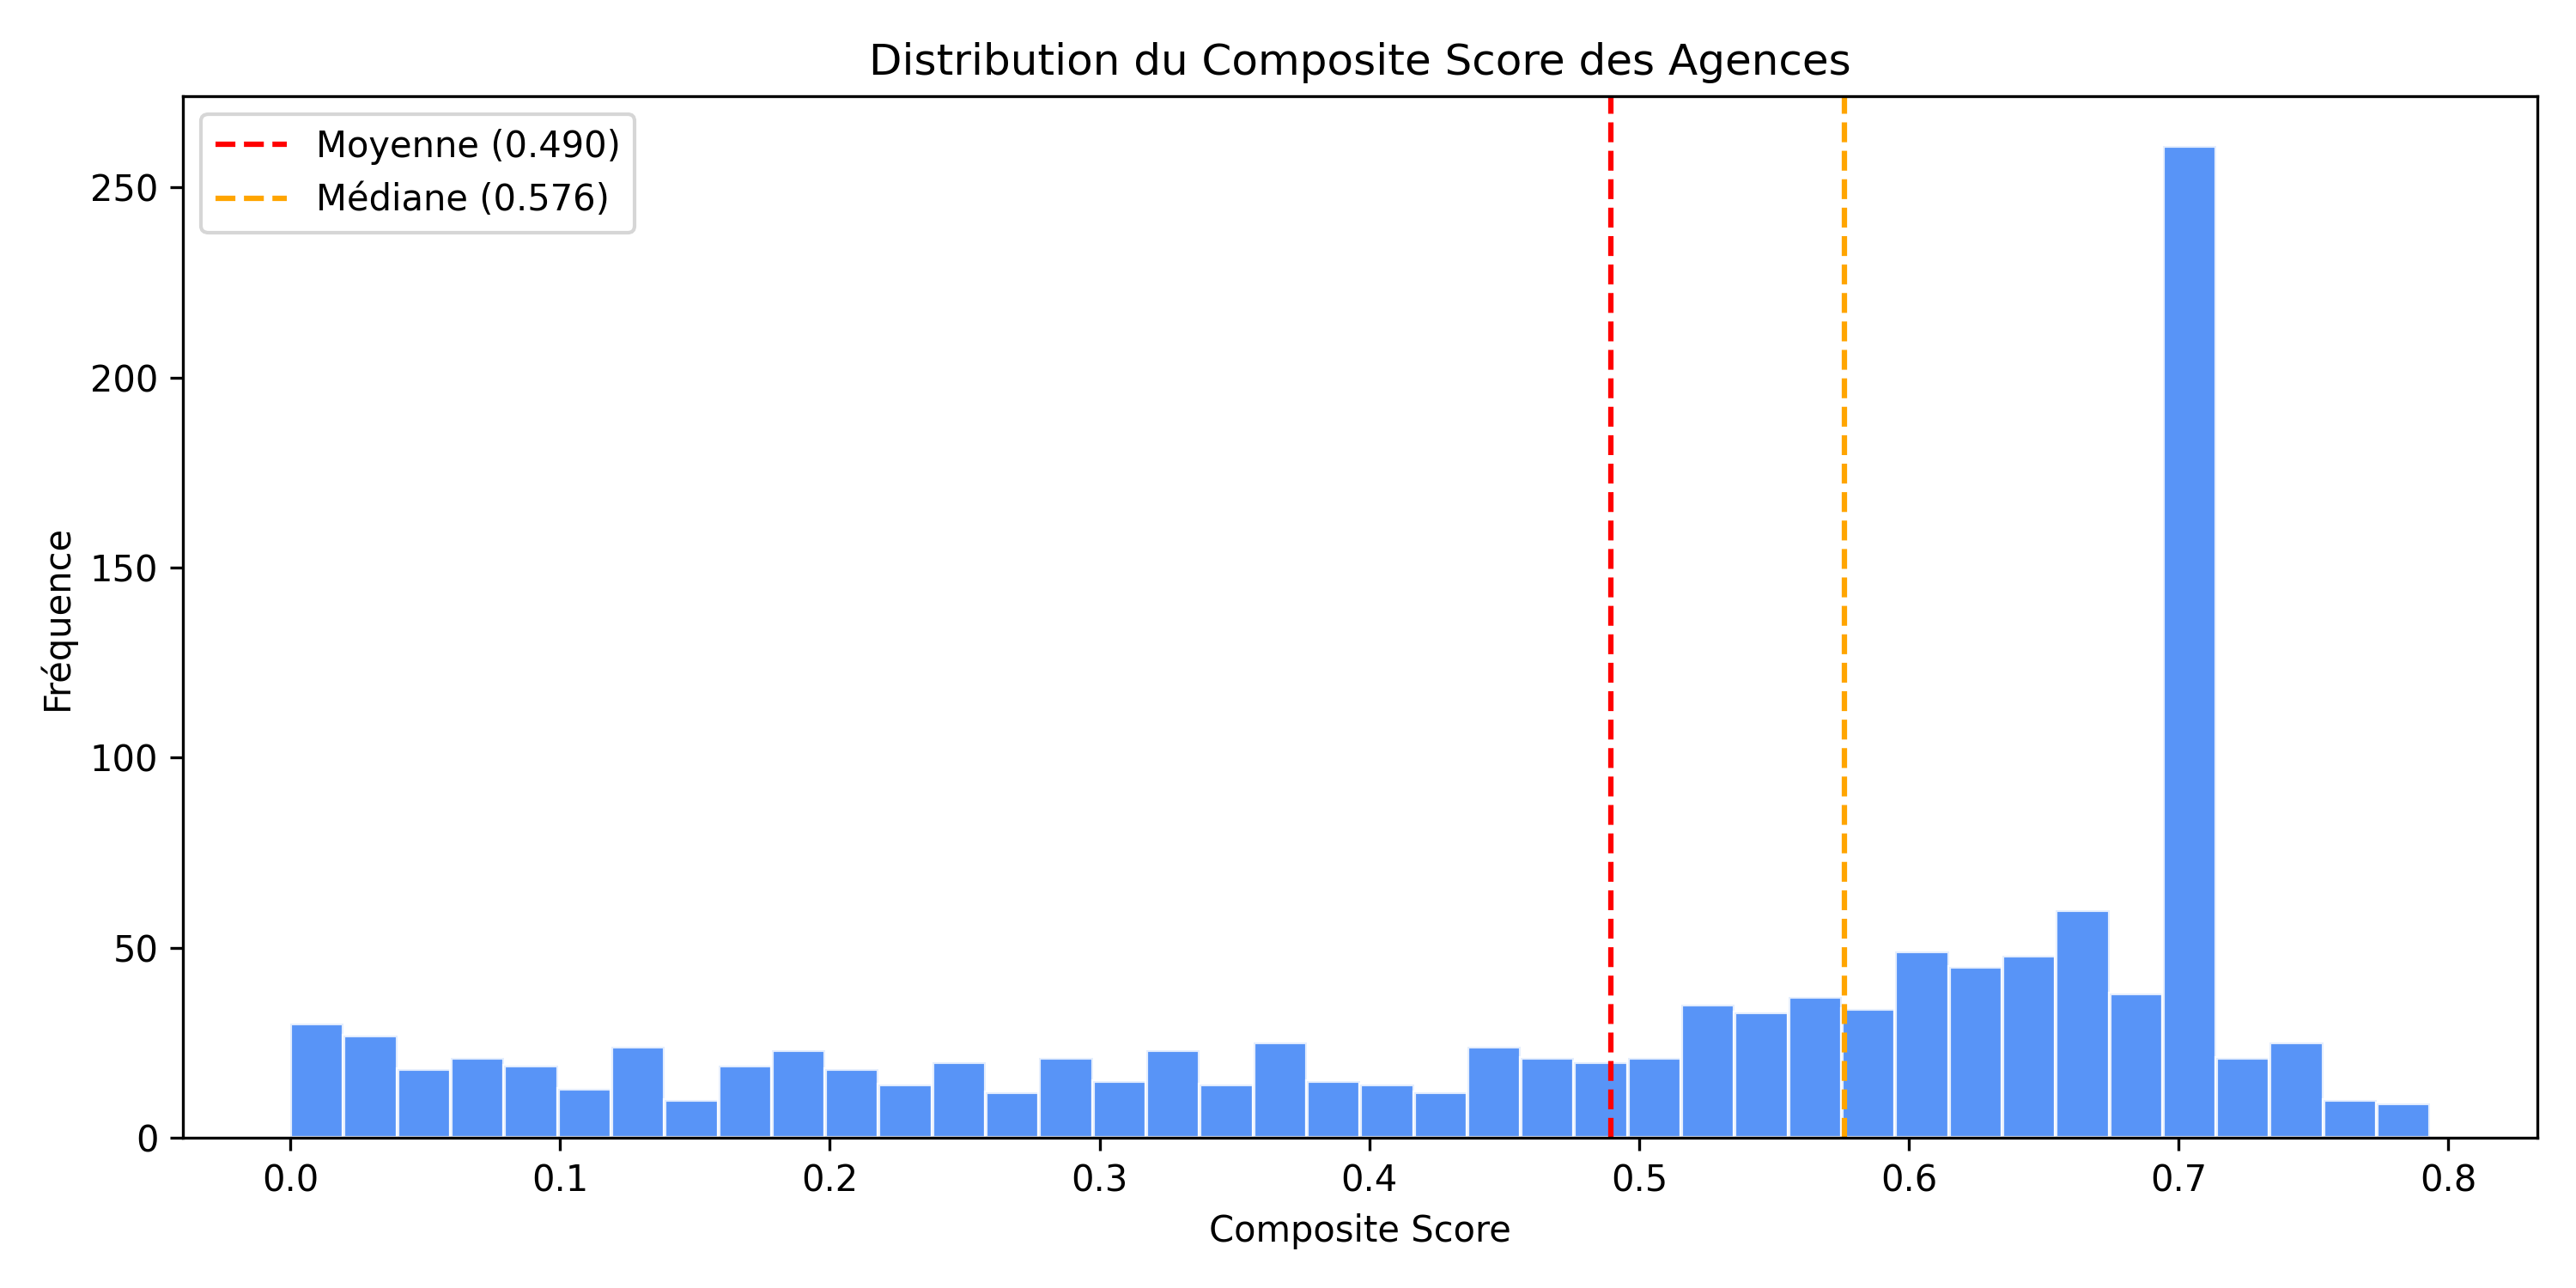
\includegraphics[width=0.9\textwidth]{figures/composite_score_dist.png}
    \caption{Distribution du Composite Score}
    \vspace{0.2cm}
    \begin{minipage}{\textwidth}
    \textbf{Description :} Cet histogramme illustre la répartition globale du score composite calculé sur l'ensemble des 1\,196 agences du réseau Attijariwafa Bank. Ce score agrège six dimensions spatiales (attractivité commerciale, résidentielle, bureaux, accessibilité, compétition et cannibalisation). La distribution met en évidence la forte hétérogénéité du réseau, avec une polarisation entre les agences urbaines bénéficiant d'un score élevé et les agences isolées ou rurales pénalisées par un faible potentiel géographique.
    \end{minipage}
    \label{fig:architecture_globale}
\end{figure}

\FloatBarrier

%=============================================================================%
\section{Orchestration et Ingénierie des Données (Tronc Commun)}
%=============================================================================%

L'intelligence spatiale repose sur la granularité et la fraîcheur des données Points of Interest (POI). Le processus d'ingénierie se divise en trois phases critiques formant un pipeline ETL (Extract-Transform-Load) complet.

\subsection{Phase d'Extraction : Collecte Multi-Sources}

La couverture exhaustive du territoire marocain nécessite l'agrégation de trois sources de données hétérogènes, chacune apportant une couche d'information complémentaire :

\begin{enumerate}
    \item \textbf{Geofabrik (Données Statiques Lourdes) :} Extraction de fichiers \texttt{.osm.pbf} régionaux issus d'OpenStreetMap \cite{openstreetmap}, contenant les infrastructures gouvernementales, hospitalières et éducatives. Ces données, mises à jour trimestriellement, constituent la couche structurelle stable de notre modèle spatial.
    \item \textbf{OpenStreetMap via Overture Maps (Données Semi-Statiques) :} Utilisation de l'outil en ligne de commande \texttt{overturemaps} pour extraire des données au format \texttt{geoparquet} dans un cadre englobant (Bounding Box) couvrant le Maroc : $[-13.2, 27.6, -0.9, 35.9]$. Ces données fournissent les réseaux routiers, les zones résidentielles et les points de transport.
    \item \textbf{Google Maps (Scraping Dynamique) :} Pour les commerces à forte volatilité temporelle (cafés, restaurants, nouvelles franchises, agences concurrentes), les bases open-source sont systématiquement obsolètes. Nous avons donc développé un scraper personnalisé.
\end{enumerate}

\subsection{Le Scraper Google Maps : Architecture et Tolérance aux Pannes}

Le scraper (\texttt{maps.py}) constitue l'innovation technique majeure du pipeline de données. Son architecture repose sur trois piliers :

\textbf{1. Heuristique de Quadrillage Spatial.} Le territoire marocain est divisé en une grille régulière de pas $\Delta = 0.3$ degrés en latitude et longitude. Pour chaque cellule $(lat_i, lon_j)$ et pour chacun des 30 mots-clés de recherche (``restaurant'', ``hospital'', ``bank'', etc.), le script génère une URL de recherche Google Maps de la forme :
\begin{center}
\texttt{https://www.google.com/maps/search/\{query\}/@\{lat\},\{lon\},13z}
\end{center}

\textbf{2. Interaction Dynamique via Selenium WebDriver.} Google Maps étant une Single Page Application (SPA) entièrement rendue côté client par JavaScript, les méthodes classiques de scraping HTTP (\texttt{requests}, \texttt{BeautifulSoup}) sont inopérantes. Le script instancie un navigateur Chrome en mode \textit{headless} via \texttt{Selenium}, puis exécute des injections JavaScript directes :
\begin{verbatim}
    arguments[0].scrollTop += 800
\end{verbatim}
Cette instruction force le défilement du panneau de résultats (\texttt{div[@role="feed"]}), déclenchant les requêtes AJAX asynchrones qui chargent les résultats suivants.

\textbf{3. Système de Checkpoints (Tolérance aux Pannes).} L'opération de scraping national prenant plusieurs heures, un mécanisme de reprise est indispensable. Chaque triplet $(lat, lon, query)$ réussi est enregistré dans le fichier \texttt{scraper\_checkpoint.txt}. Au redémarrage, ces clés sont chargées dans une structure de type \texttt{set} en Python, offrant une complexité de recherche en $O(1)$ et permettant au script de reprendre exactement là où il s'était interrompu. Les données brutes sont sauvegardées par lots de 50 enregistrements pour minimiser la perte en cas d'interruption brutale.

\subsection{Phase de Transformation : Nettoyage et Fusion (\texttt{cleanall.py})}

L'unification de ces trois sources disparates pose des défis stricts de standardisation que le pipeline résout en trois étapes :

\begin{enumerate}
    \item \textbf{Résolution des Encodages :} Les données issues du web contiennent fréquemment des octets corrompus (ex: \texttt{0xe9} pour le caractère ``é''). Le pipeline force la lecture via l'encodage \texttt{latin1} puis effectue la sauvegarde finale en \texttt{UTF-8} universel, garantissant la compatibilité avec les bibliothèques d'analyse.
    \item \textbf{Normalisation des Schémas :} Chaque source utilise des noms de colonnes différents. Le script standardise les champs vers un schéma commun : \texttt{name}, \texttt{category}, \texttt{latitude}, \texttt{longitude}.
    \item \textbf{Dédoublonnage Géométrique :} Un même commerce peut exister dans la base OSM et Google Maps sous des noms différents (``Pharmacie Centrale'' vs ``Pharm. Centrale''). Le dédoublonnage textuel étant inopérant, nous utilisons la vérité terrain géométrique via \texttt{drop\_duplicates(subset=['latitude','longitude'], keep='first')}, garantissant l'unicité stricte des coordonnées GPS.
\end{enumerate}

Le résultat final est un fichier unifié \texttt{merged\_data\_clean.csv} constituant la base de référence pour toute l'analyse spatiale.

\subsection{Phase de Chargement : Ingénierie des Caractéristiques Spatiales}

Conformément à la première loi de la géographie de Tobler \cite{tobler1970}, qui stipule que les entités proches sont plus fortement corrélées que les entités éloignées, nous transformons un simple point GPS en vecteur de caractéristiques exploitable par nos algorithmes via une \textbf{agrégation radiale}. Pour chaque agence (UC1) ou candidat (UC2), l'algorithme compte les densités de POI à l'intérieur d'isochrones circulaires de rayons 500m, 1km et 2km, générant un vecteur $X_i \in \mathbb{R}^6$ composé des six scores suivants :

\begin{table}[h]
\centering
\begin{tabular}{|l|l|p{7cm}|}
\hline
\textbf{Variable} & \textbf{Type} & \textbf{Description} \\ \hline
\texttt{score\_commercial} & Attractivité & Densité pondérée des commerces (restaurants, malls, marchés) dans un rayon de 1km \\ \hline
\texttt{score\_office} & Attractivité & Densité des bureaux et administrations à 1km \\ \hline
\texttt{score\_residential} & Attractivité & Densité des zones résidentielles à 1km \\ \hline
\texttt{score\_accessibility} & Attractivité & Proximité des transports en commun (gares, arrêts de bus) à 500m \\ \hline
\texttt{score\_competition} & Risque & Nombre de banques concurrentes dans un rayon de 1km \\ \hline
\texttt{score\_cannibalization} & Risque & Nombre d'agences Attijariwafa Bank dans un rayon de 2km \\ \hline
\end{tabular}
\caption{Description des 6 caractéristiques spatiales constituant le vecteur d'entrée des modèles.}
\label{tab:features}
\end{table}

Ces six scores sont ensuite combinés en un \textbf{Composite Score} global via une combinaison linéaire pondérée :
\begin{equation}
S_{composite} = \alpha \cdot S_{comm} + \beta \cdot S_{off} + \gamma \cdot S_{res} + \delta \cdot S_{acc} - \epsilon \cdot S_{comp} - \zeta \cdot S_{can}
\label{eq:composite}
\end{equation}
où les coefficients $(\alpha, \beta, \gamma, \delta, \epsilon, \zeta)$ reflètent l'importance relative de chaque dimension pour l'activité bancaire. La soustraction des scores de compétition et de cannibalisation pénalise les zones saturées.

\begin{figure}[h]
    \centering
    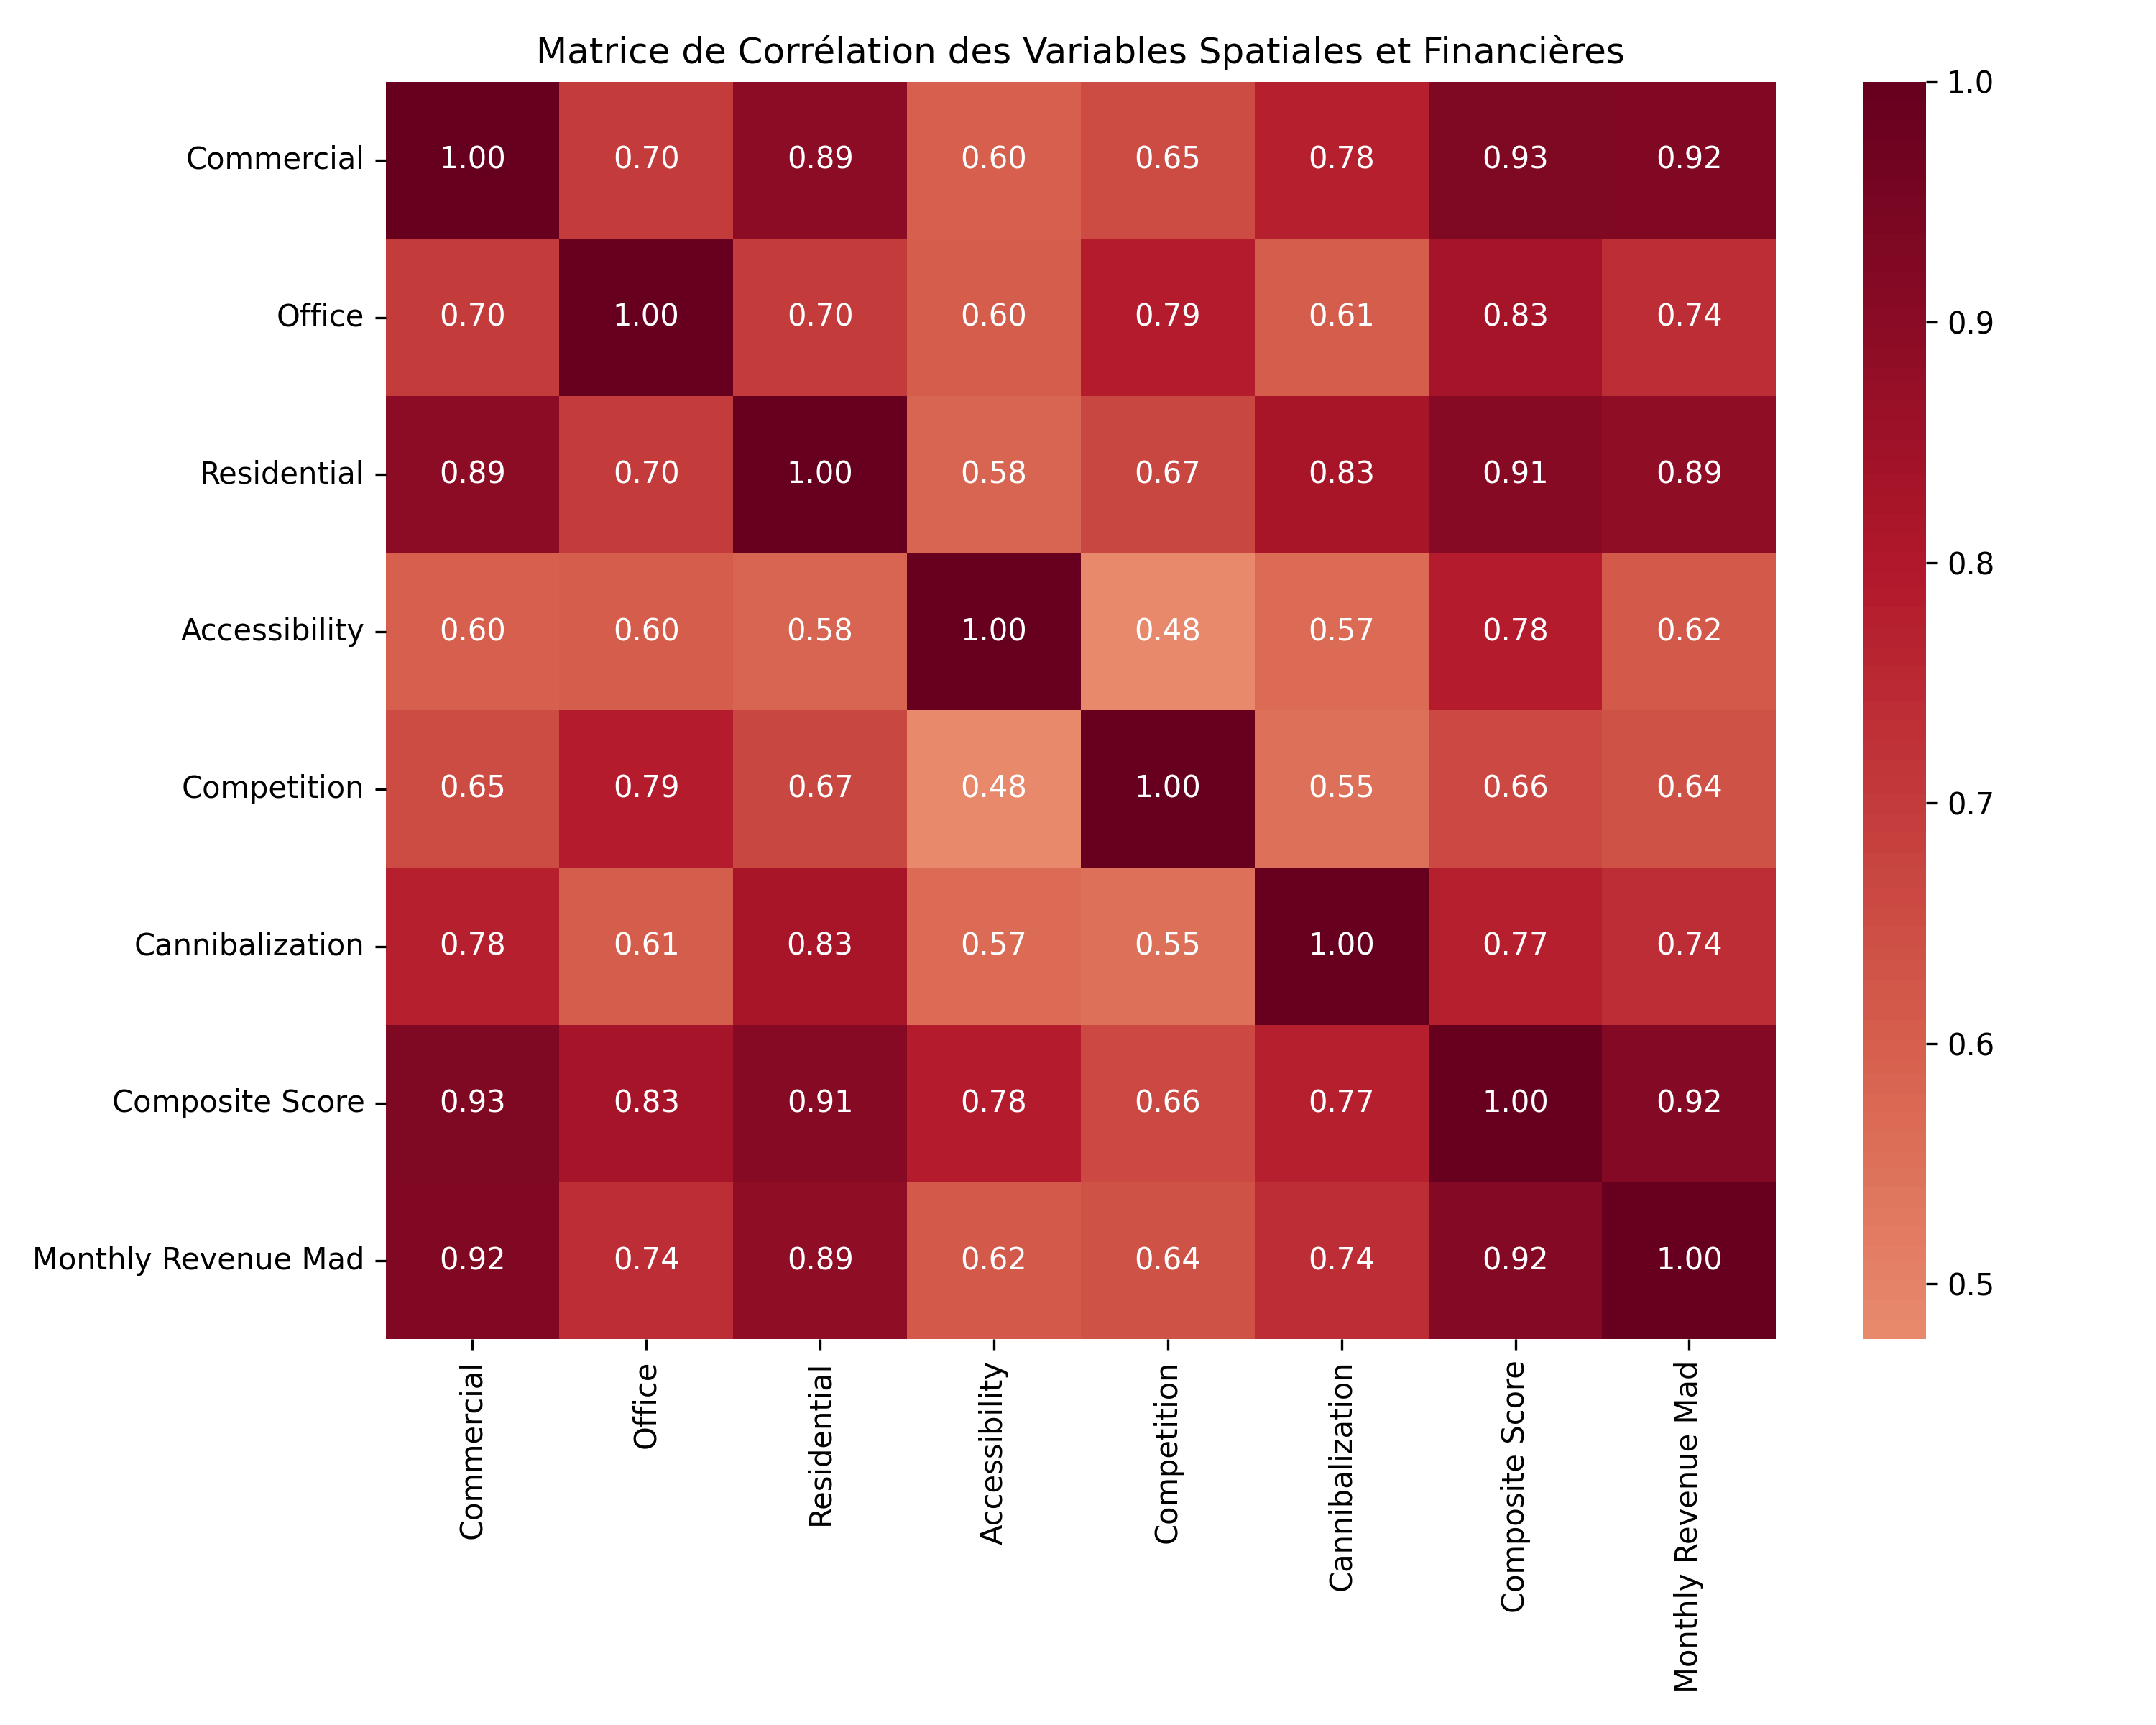
\includegraphics[width=0.75\textwidth]{figures/correlation_heatmap.png}
    \caption{Matrice de corrélation de Pearson}
    \vspace{0.2cm}
    \begin{minipage}{\textwidth}
    \textbf{Description :} Cette carte de chaleur (heatmap) présente les coefficients de corrélation linéaire de Pearson entre les différents scores spatiaux calculés et la variable cible. Elle permet de vérifier l'absence de colinéarité excessive entre nos variables explicatives et confirme visuellement quelles caractéristiques (comme le score commercial) ont l'impact statistique le plus fort sur la rentabilité d'une agence.
    \end{minipage}
    \label{fig:correlation}
\end{figure}

\FloatBarrier

%=============================================================================%
\section{Cas d'Usage 1 : Évaluation et Optimisation du Réseau Existant}
%=============================================================================%

Ce premier cas d'usage vise à auditer le réseau bancaire actuel en combinant apprentissage non supervisé (segmentation) et supervisé (prédiction des revenus), aboutissant à un outil d'aide à la décision stratégique.

\subsection{Apprentissage Non Supervisé : Segmentation par K-Means}

\subsubsection{Méthodologie et Prétraitement}

La première étape de l'évaluation consiste à identifier des profils d'agences homogènes. Comparer naïvement une agence de centre d'affaires à une agence rurale serait une erreur méthodologique fondamentale.

Préalablement au clustering, la matrice des scores $X \in \mathbb{R}^{1198 \times 6}$ subit une transformation Z-Score via \texttt{StandardScaler} :
\begin{equation}
z_{ij} = \frac{x_{ij} - \bar{x}_j}{\sigma_j}
\end{equation}
Cette normalisation est indispensable car la distance Euclidienne utilisée par K-Means est sensible aux échelles : sans standardisation, les variables à forte variance numérique domineraient le calcul des centroïdes.

L'algorithme K-Means est exécuté avec $K=5$ clusters et $n\_init=10$ initialisations aléatoires pour éviter la convergence vers un minimum local de la fonction objectif de Lloyd.

\subsubsection{Résultats du Clustering}

L'algorithme identifie cinq profils spatiaux distincts au sein du réseau. Le tableau~\ref{tab:clusters} résume les caractéristiques de chaque cluster :

\begin{table}[h]
\centering
\begin{tabular}{|l|c|c|}
\hline
\textbf{Profil (Cluster)} & \textbf{Nombre d'Agences} & \textbf{Score Composite Moyen} \\ \hline
High Performer & 396 & 0.686 \\ \hline
Commercial Hub & 294 & 0.614 \\ \hline
Residential Anchor & 181 & 0.412 \\ \hline
Underperformer & 119 & 0.311 \\ \hline
At Risk / Redundant & 208 & 0.109 \\ \hline
\end{tabular}
\caption{Répartition des 1\,196 agences dans les 5 clusters K-Means.}
\label{tab:clusters}
\end{table}

\subsubsection{Réduction de Dimensionnalité : Analyse en Composantes Principales}

Pour visualiser la séparation des clusters dans un espace interprétable, nous appliquons une ACP (Analyse en Composantes Principales) qui projette l'espace $\mathbb{R}^6$ vers $\mathbb{R}^2$. Les deux premières composantes capturent respectivement \textbf{72.5\%} et \textbf{10.1\%} de la variance totale, soit un cumul de \textbf{82.6\%}, justifiant pleinement la projection bidimensionnelle.

\begin{figure}[h]
    \centering
    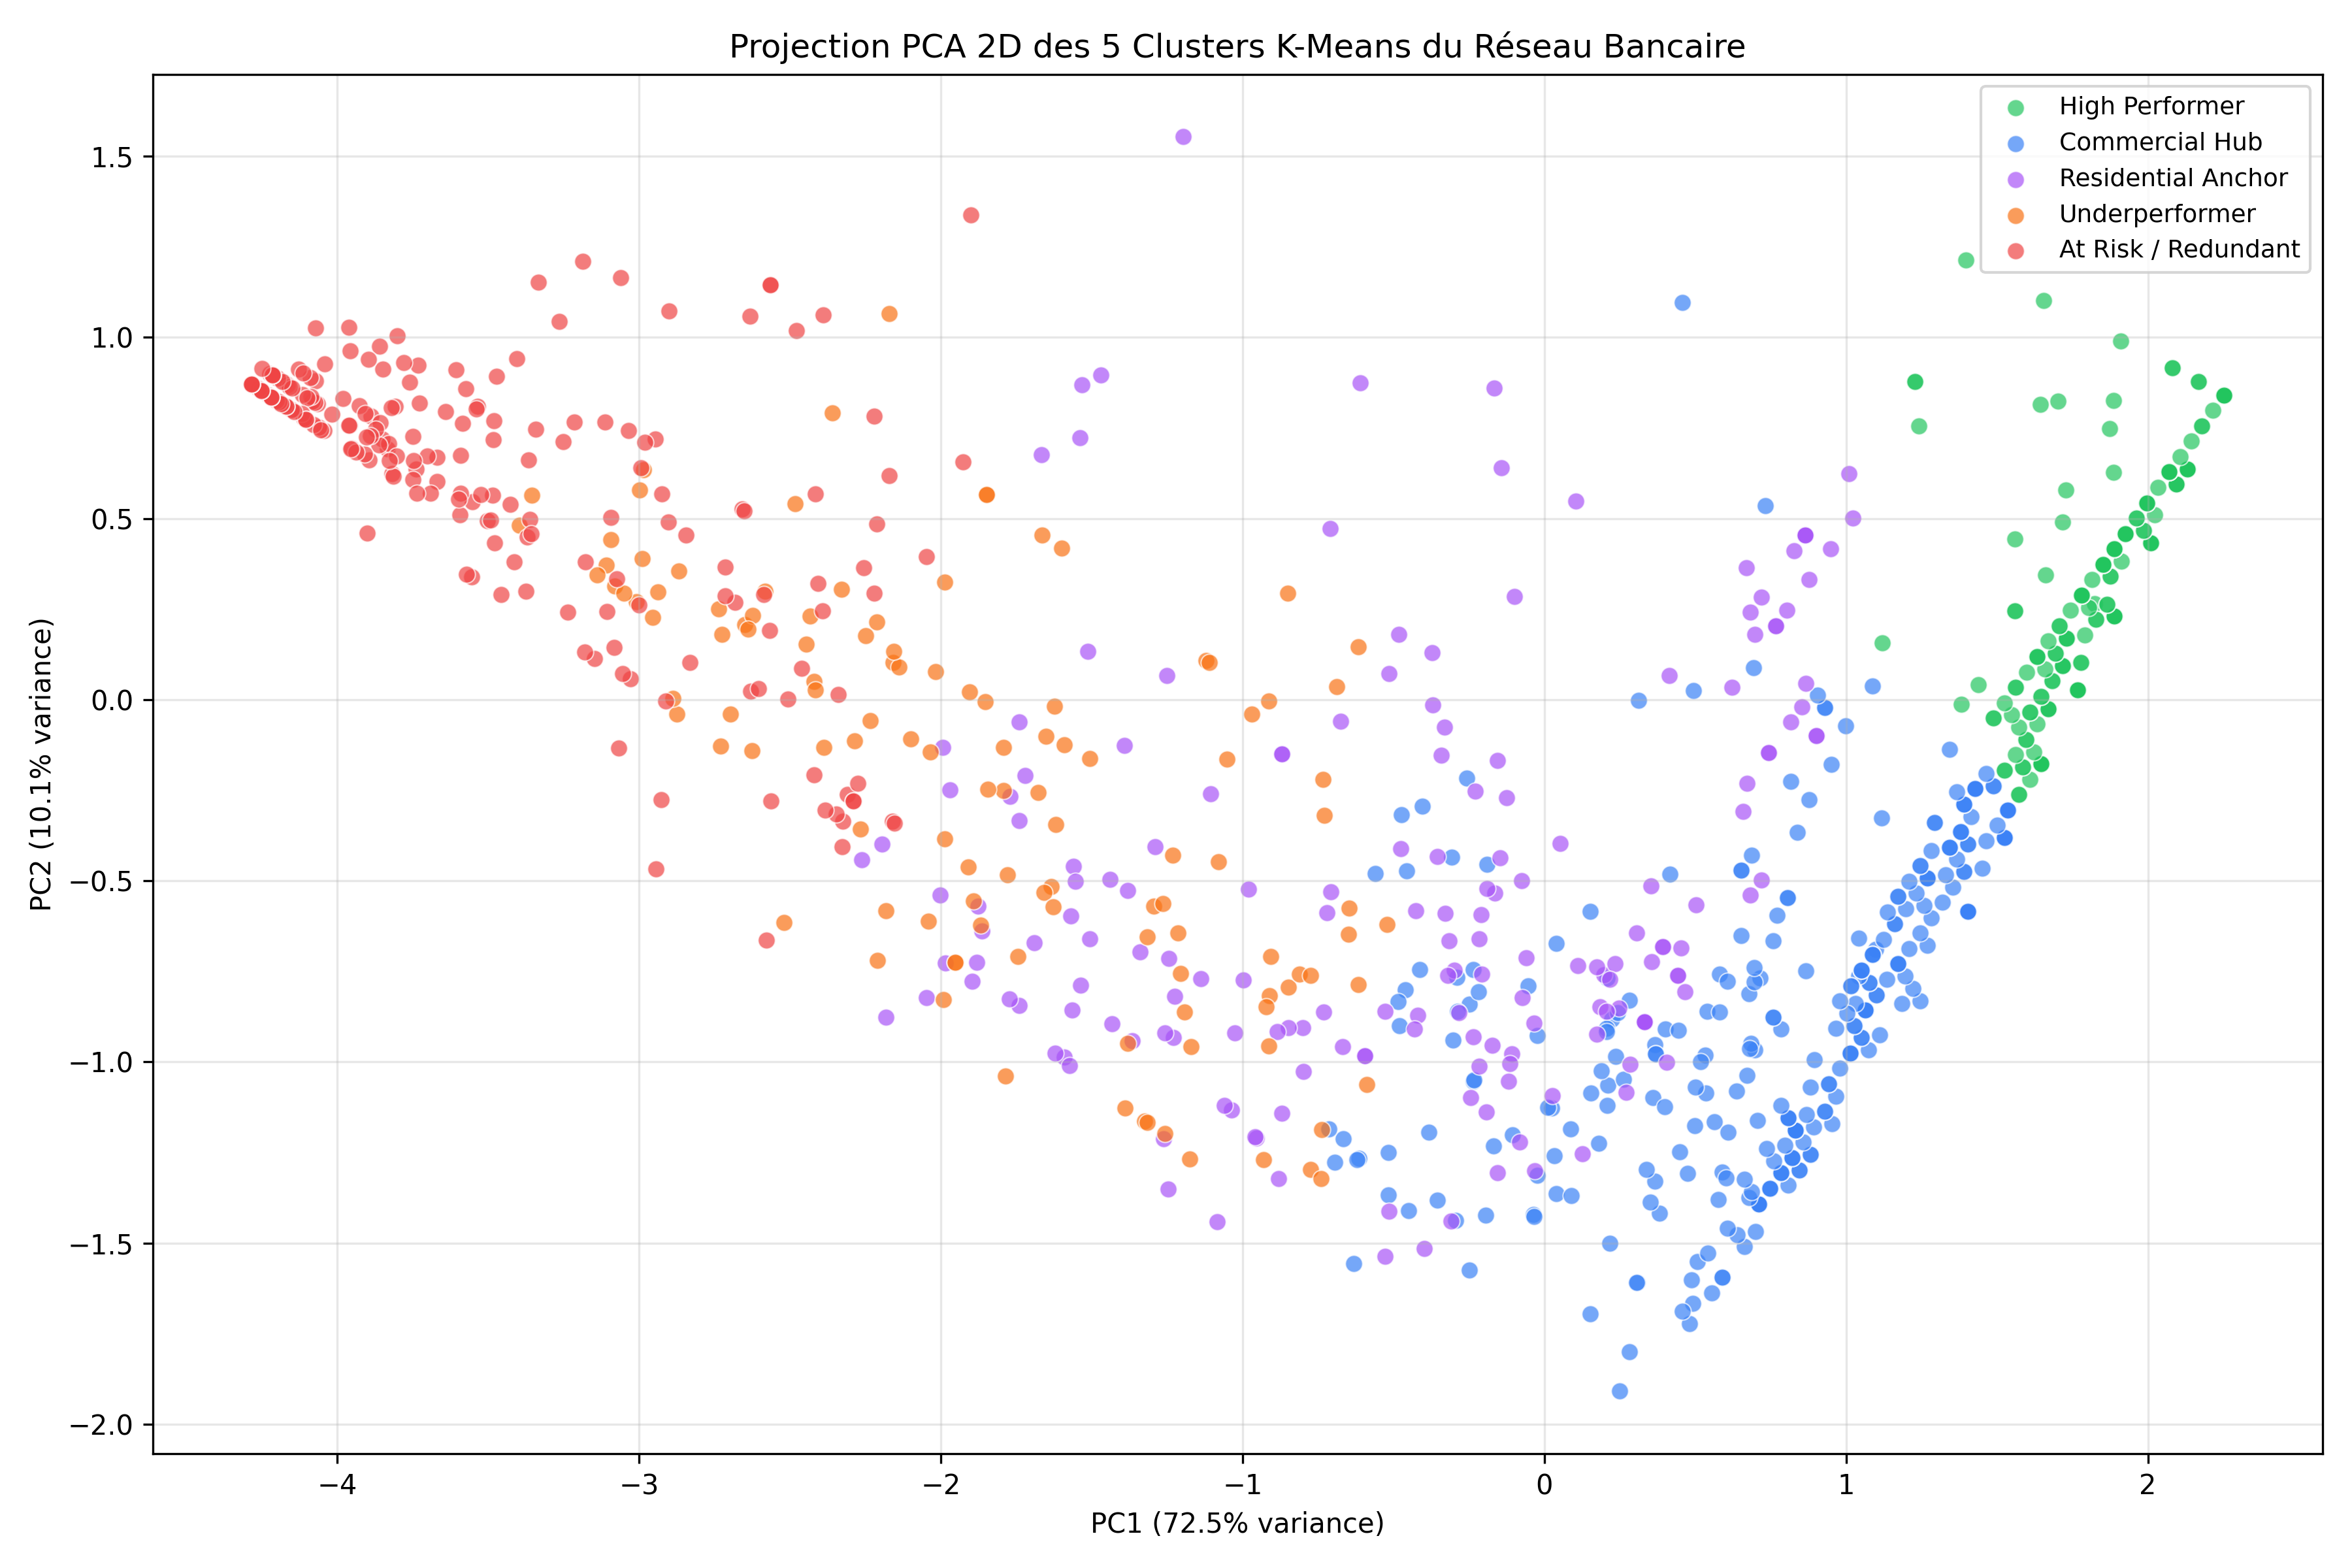
\includegraphics[width=0.85\textwidth]{figures/pca_clusters.png}
    \caption{Projection PCA 2D des 5 clusters K-Means}
    \vspace{0.2cm}
    \begin{minipage}{\textwidth}
    \textbf{Description :} Cette visualisation bidimensionnelle est le résultat d'une Analyse en Composantes Principales (ACP) appliquée après l'algorithme K-Means. L'axe principal (PC1) capture près de 73\% de la variance et sépare les zones denses des zones isolées. L'axe secondaire (PC2) différencie la vocation du quartier (commercial versus résidentiel). Les cinq couleurs représentent les cinq profils géospatiaux d'agences, montrant clairement les frontières et la densité de chaque cluster au sein du réseau.
    \end{minipage}
    \label{fig:pca_clusters}
\end{figure}

\FloatBarrier
\begin{figure}[h]
    \centering
    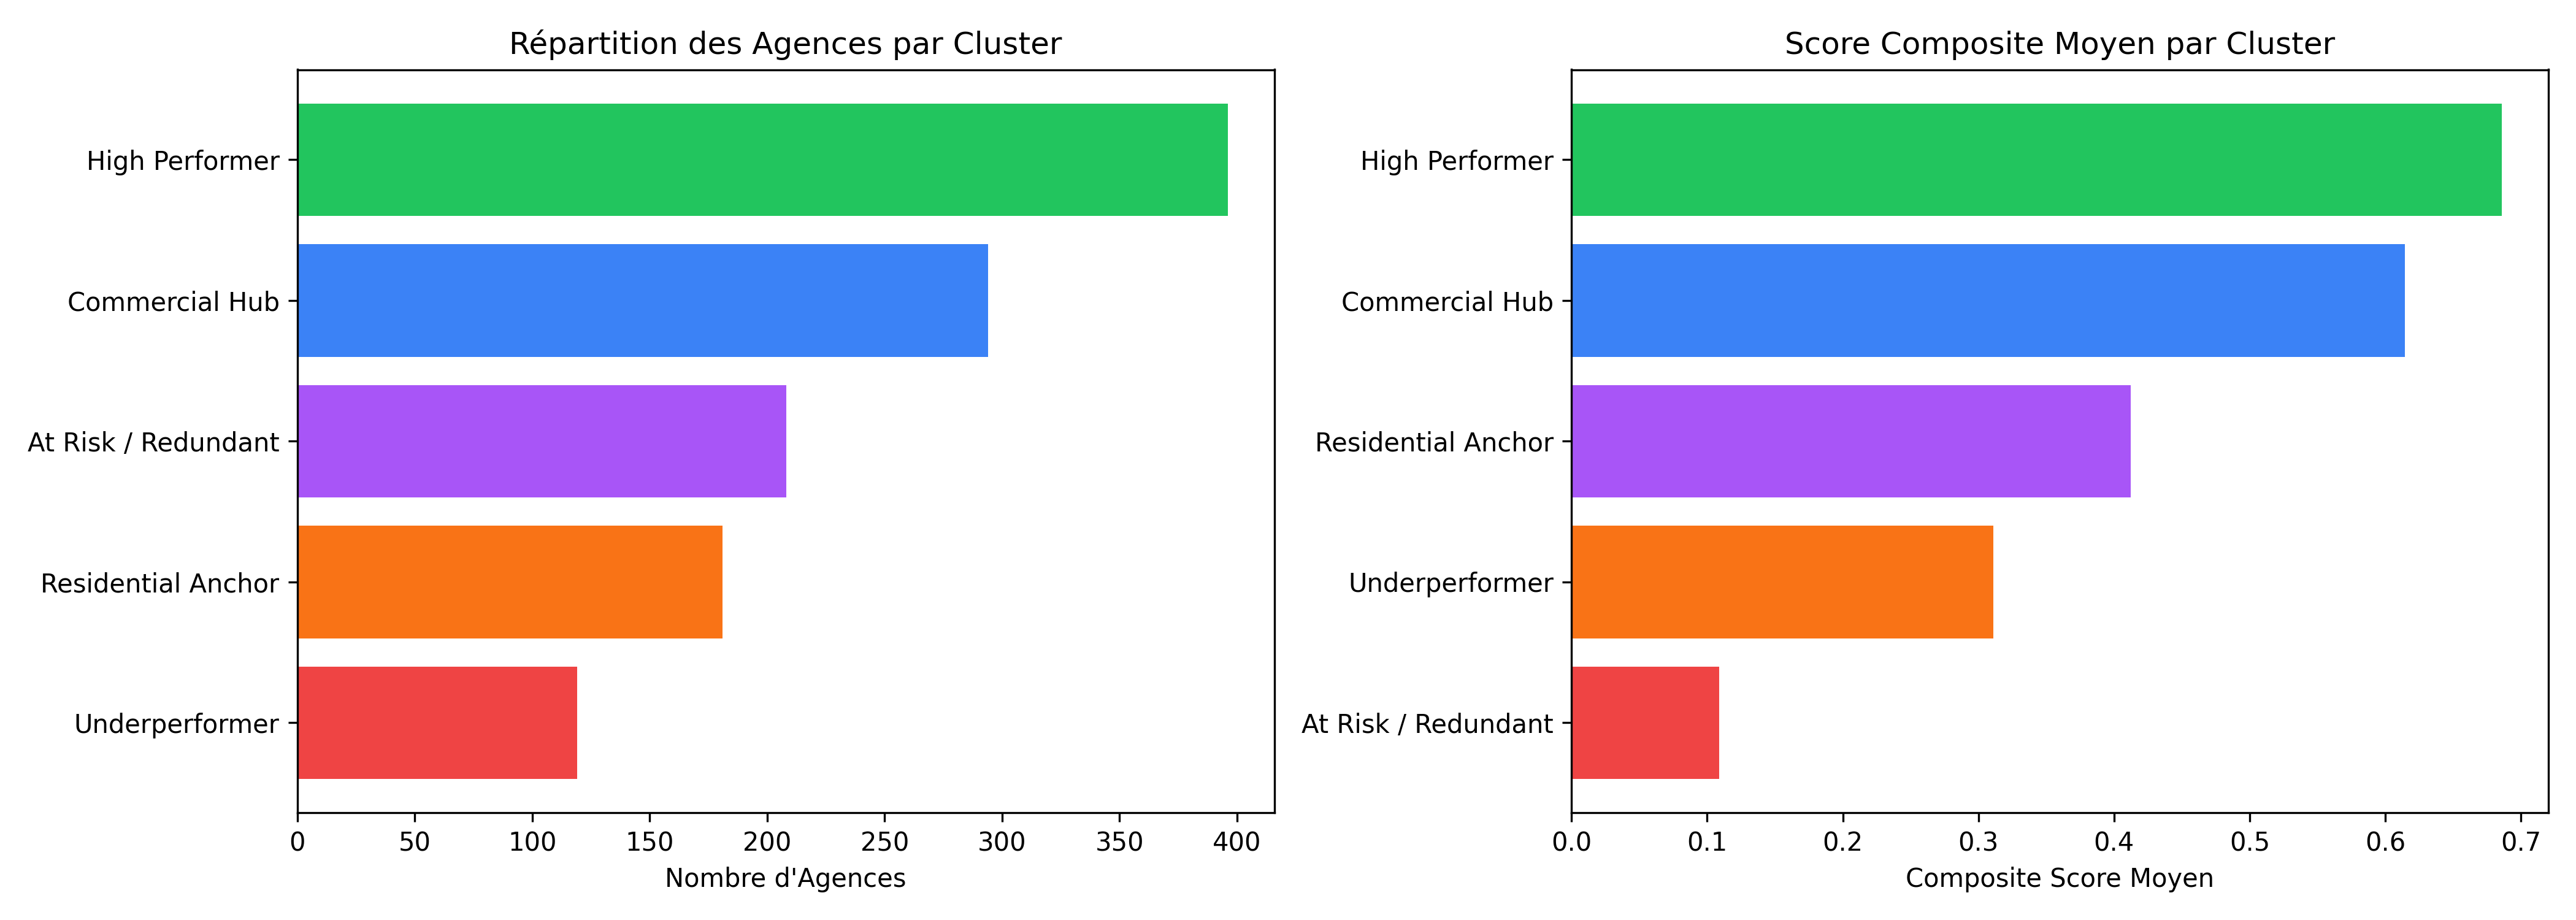
\includegraphics[width=\textwidth]{figures/cluster_distribution.png}
    \caption{Répartition et score composite moyen par cluster}
    \vspace{0.2cm}
    \begin{minipage}{\textwidth}
    \textbf{Description :} Ce diagramme en barres détaille de manière quantitative la proportion des 1\,198 agences affectées à chacun des cinq clusters identifiés. Il met également en évidence le niveau d'attractivité composite moyen pour chaque groupe. Cela permet aux décideurs de visualiser d'un seul coup d'œil le poids des High Performers par rapport aux agences At Risk ou Underperformers dans la structure globale de la banque.
    \end{minipage}
    \label{fig:cluster_dist}
\end{figure}

\FloatBarrier
\subsubsection{Profilage Multidimensionnel par Radar Charts}

Pour comprendre la signature spatiale de chaque cluster, nous utilisons des diagrammes radar (Spider Charts) représentant la moyenne de chaque score pour chaque profil. Cette visualisation confirme que :
\begin{itemize}
    \item Les \textit{High Performers} se distinguent par des scores élevés sur toutes les dimensions d'attractivité.
    \item Les \textit{Commercial Hubs} présentent une dominance marquée du score commercial mais un score résidentiel plus faible.
    \item Les agences \textit{At Risk} combinent de faibles scores d'attractivité avec une cannibalisation élevée.
\end{itemize}

\begin{figure}[h]
    \centering
    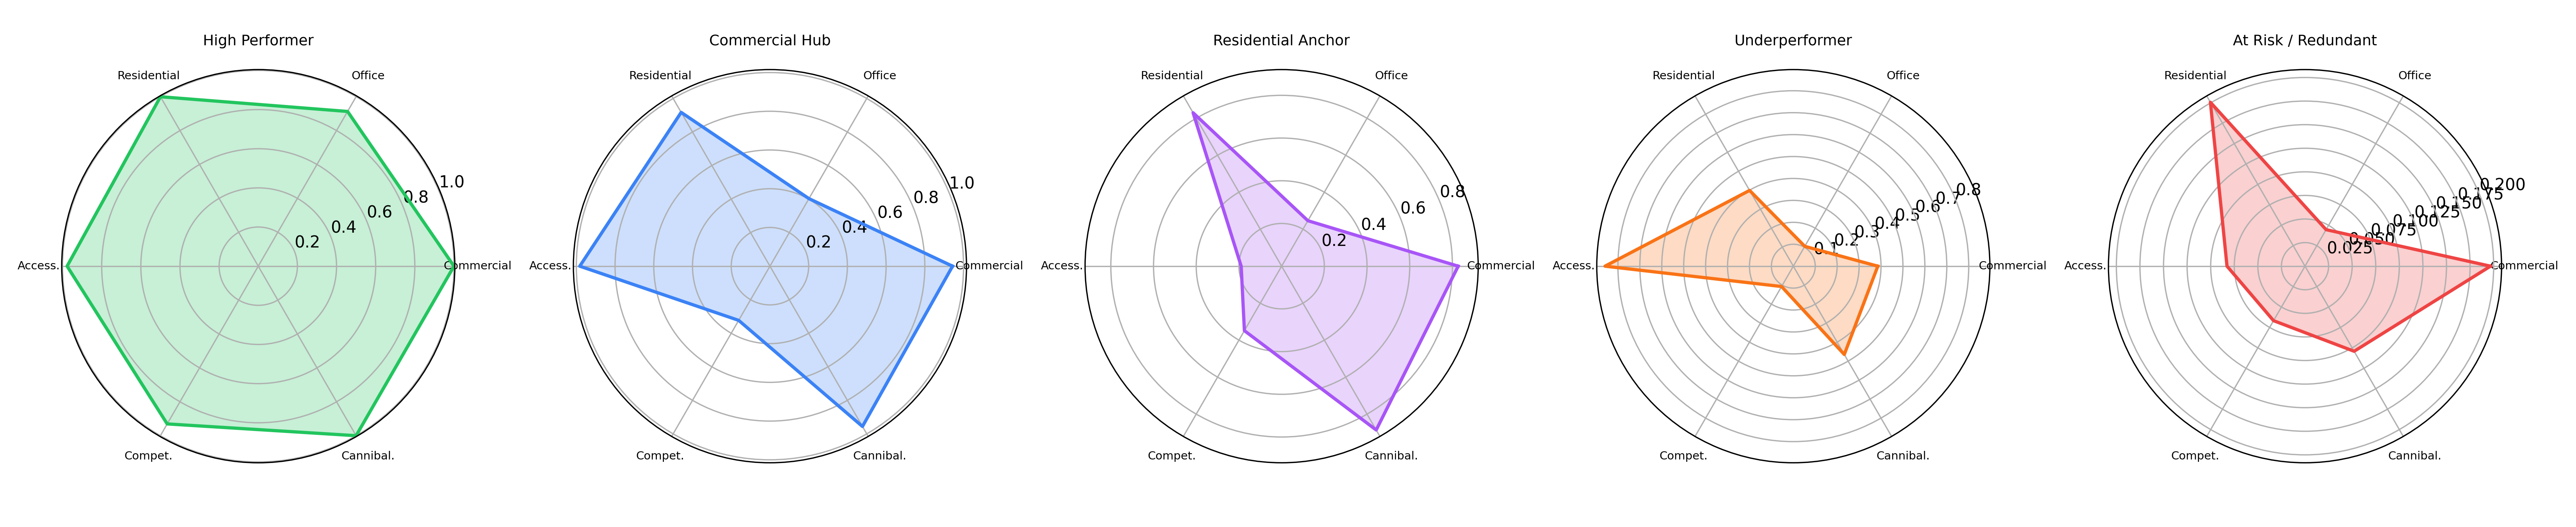
\includegraphics[width=\textwidth]{figures/cluster_radar.png}
    \caption{Diagrammes radar des 5 profils d'agences}
    \vspace{0.2cm}
    \begin{minipage}{\textwidth}
    \textbf{Description :} Ces diagrammes radar offrent une représentation multidimensionnelle de la signature spatiale moyenne de chaque cluster. Chaque axe du polygone représente la valeur moyenne d'un des six scores spatiaux. Cette visualisation permet de contraster immédiatement les points forts et faibles de chaque profil, par exemple en opposant le score commercial très élevé des Commercial Hubs à la forte densité d'habitat des Residential Anchors.
    \end{minipage}
    \label{fig:cluster_radar}
\end{figure}

\FloatBarrier


\subsection{Benchmarking Algorithmique : Prédiction des Revenus (Régression)}

Pour évaluer objectivement le potentiel théorique d'une agence, nous modélisons un problème de régression supervisée où la variable cible $Y$ est le revenu mensuel réel (en MAD), et la matrice $X$ contient les 6 scores spatiaux normalisés. L'ensemble de données ($N = 1\,196$) est partitionné en un ensemble d'entraînement (80\%) et un ensemble de test (20\%) via un échantillonnage stratifié (\texttt{random\_state=42}).

Afin de justifier scientifiquement notre choix de modèle final, nous avons conduit un benchmarking rigoureux de quatre architectures algorithmiques, couvrant le spectre complet des paradigmes de Machine Learning.

\subsubsection{Analyse de la Variable Cible}

La distribution du revenu mensuel des agences (figure~\ref{fig:revenue_dist}) présente une structure bimodale avec une concentration significative autour de 12\,000\,000 MAD et une queue de distribution vers les revenus plus faibles. La moyenne s'établit à \textbf{8\,385\,199 MAD} et la médiane à \textbf{11\,971\,900 MAD}. Cette asymétrie justifie l'utilisation de métriques robustes (MAE) en complément du RMSE.

\begin{figure}[h]
    \centering
    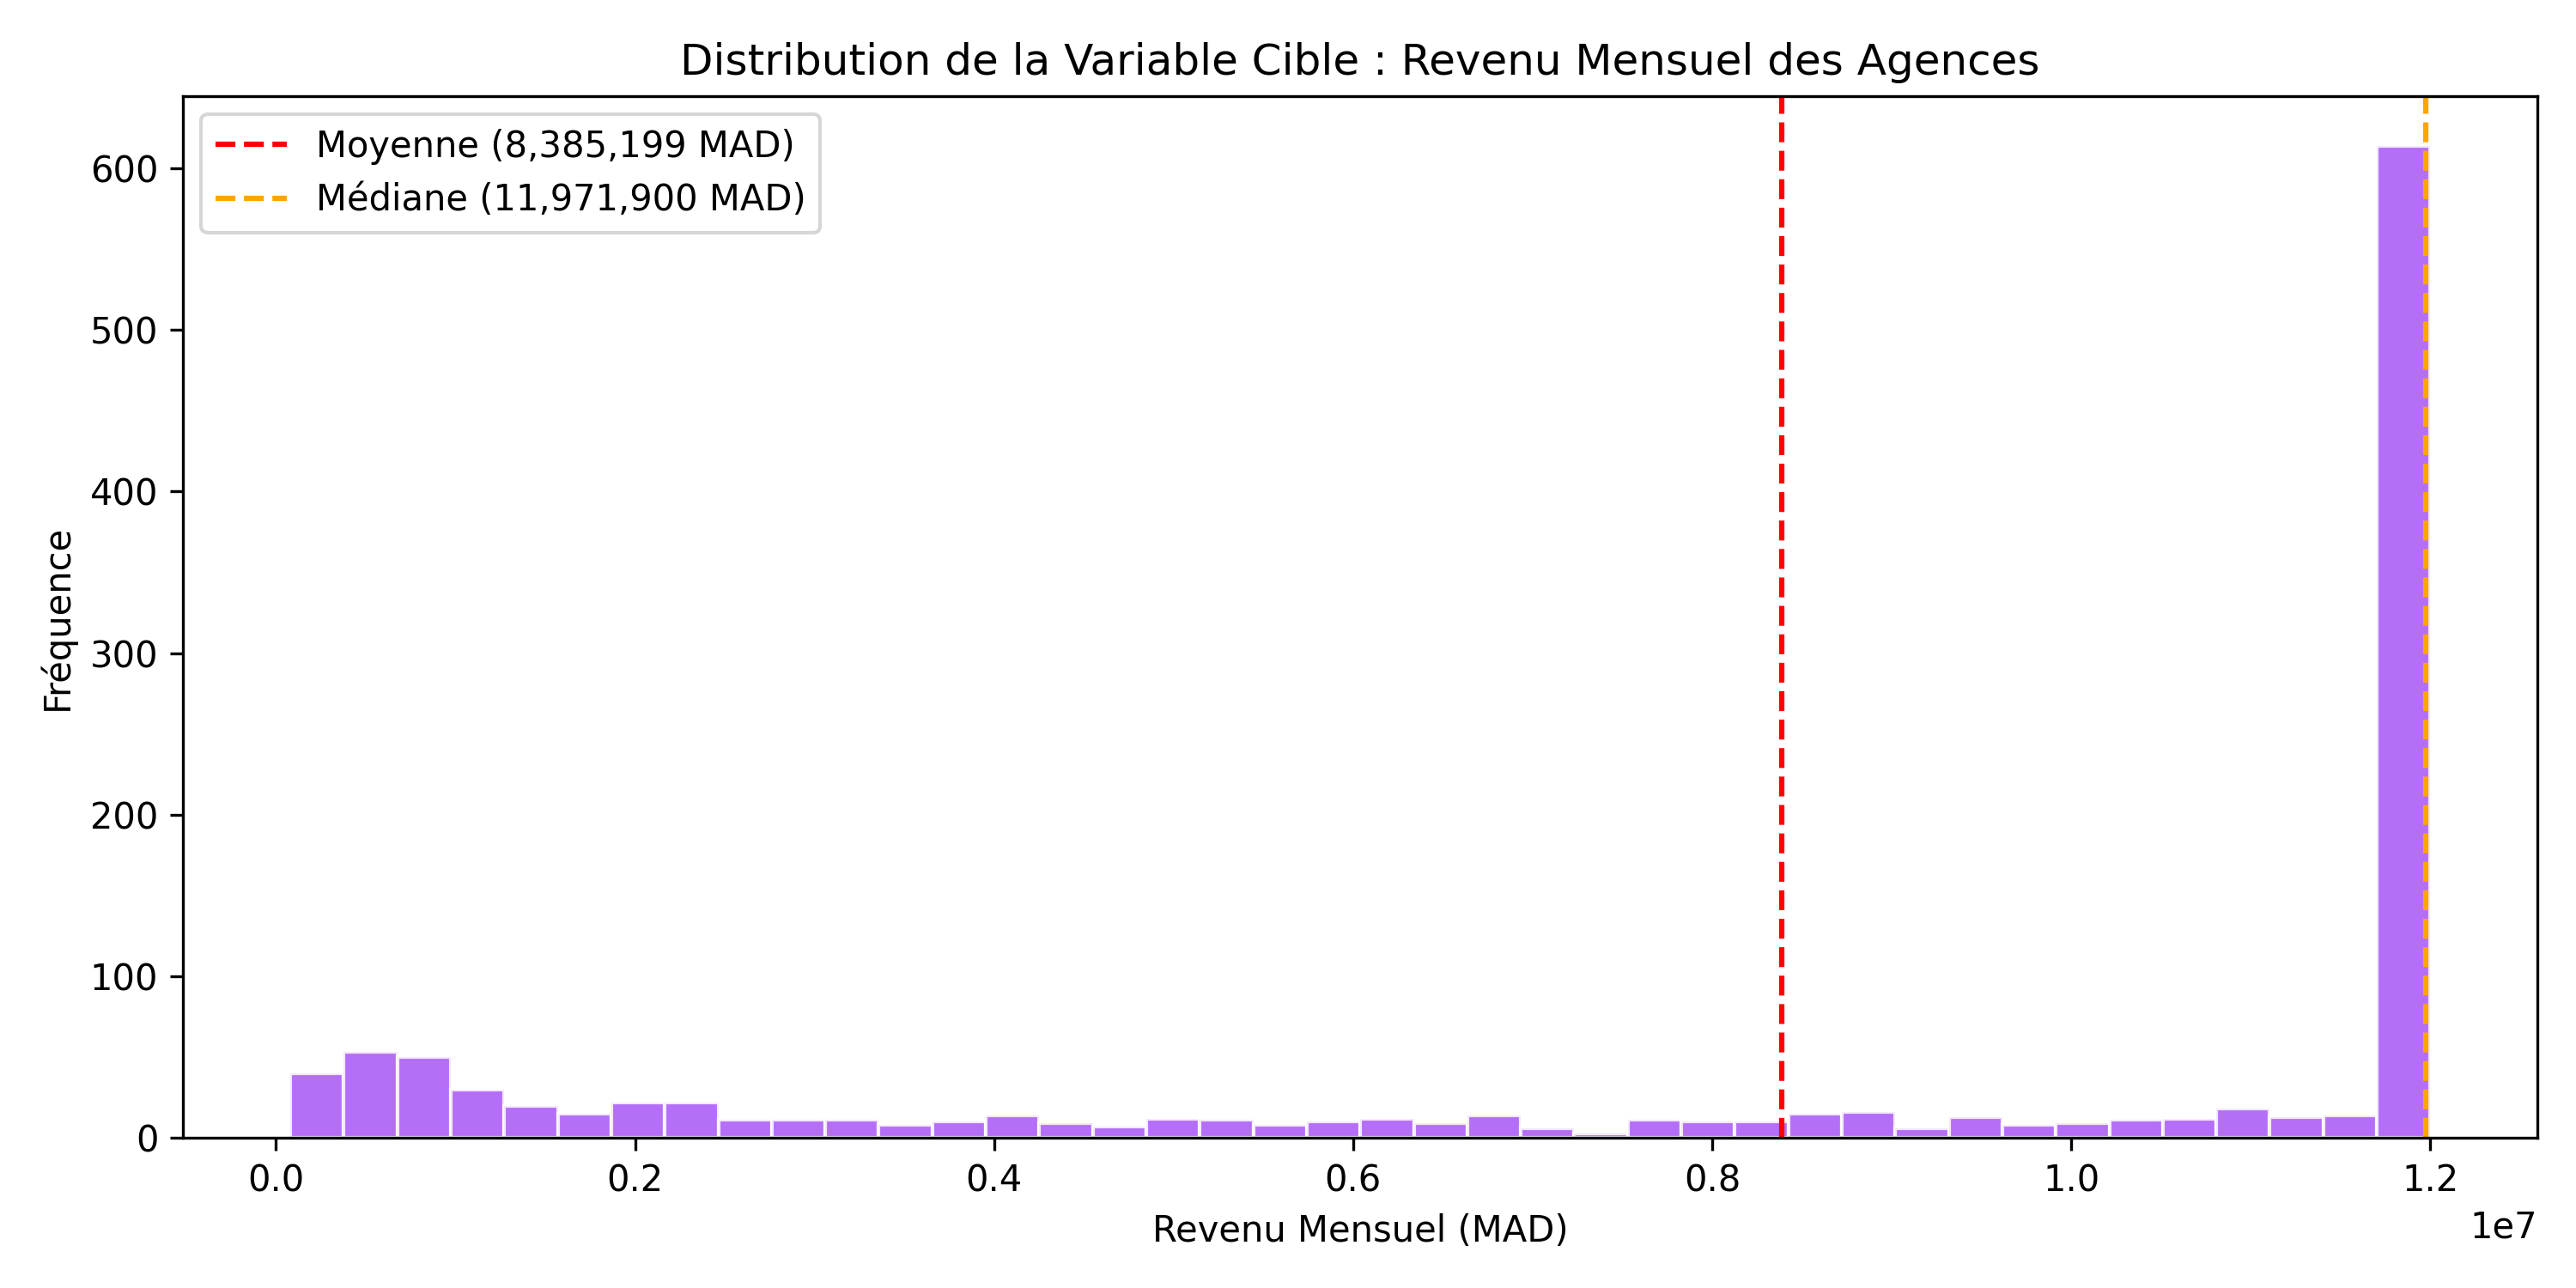
\includegraphics[width=0.85\textwidth]{figures/revenue_distribution.png}
    \caption{Distribution de la variable cible (revenu mensuel en MAD).}
    \vspace{0.2cm}
    \begin{minipage}{\textwidth}
    \textbf{Description :} Cet histogramme détaille la répartition des revenus mensuels réels générés par les agences du réseau bancaire, qui constitue la variable cible de nos modèles d'apprentissage automatique. La forme de la distribution montre une asymétrie avec une queue étalée vers la droite et une structure bimodale, justifiant ainsi le choix de modèles robustes et de métriques d'évaluation adaptées pour gérer ces valeurs extrêmes de rentabilité.
    \end{minipage}
    \label{fig:revenue_dist}
\end{figure}

\FloatBarrier
\subsubsection{Modèle 1 : Régression Linéaire par Moindres Carrés Ordinaires (OLS)}

Le modèle OLS constitue notre ligne de base (\textit{baseline}). Il estime un hyperplan dans $\mathbb{R}^6$ minimisant la somme des carrés des résidus. Bien que théoriquement optimal sous les hypothèses de Gauss-Markov (homoscédasticité, indépendance, normalité des résidus), ces conditions sont rarement satisfaites dans un contexte géospatial où les interactions entre variables sont hautement non-linéaires.

\subsubsection{Modèle 2 : Régression Ridge ($L_2$)}

La régression Ridge ajoute une pénalité de norme $L_2$ au terme de perte OLS :
\begin{equation}
\mathcal{L}_{Ridge} = \sum_{i=1}^{N} (y_i - \hat{y}_i)^2 + \lambda \sum_{j=1}^{p} \beta_j^2
\end{equation}
Le terme de régularisation $\lambda$ réduit la variance des coefficients en les contraignant vers zéro, sans les annuler. Avec $\lambda = 1.0$, ce modèle vise à améliorer la généralisation par rapport à l'OLS en réduisant le surapprentissage.

\subsubsection{Modèle 3 : Random Forest (Bagging d'Arbres de Décision)}

Le Random Forest agrège $B = 100$ arbres de décision profonds, chacun entraîné sur un échantillon bootstrap distinct du dataset. Contrairement aux modèles linéaires, cette architecture capture nativement les interactions non-linéaires (ex: ``le revenu explose uniquement si le score commercial $> 0.5$ ET la cannibalisation $< 0.2$''). La décorrélation des arbres (via la sélection aléatoire de $\sqrt{p}$ variables à chaque nœud) réduit la variance de l'estimateur sans augmenter le biais.

\subsubsection{Modèle 4 : XGBoost (Extreme Gradient Boosting)}

XGBoost construit ses arbres de manière séquentielle. À l'itération $t$, le nouvel arbre $f_t$ est mathématiquement entraîné pour prédire le résidu d'erreur (gradient de la fonction de perte) des arbres précédents. L'utilisation de l'approximation de Taylor au second ordre (calcul du Hessien) permet une convergence optimale. La régularisation intégrée ($L_1$ et $L_2$ sur les poids des feuilles) confère une robustesse supérieure face aux valeurs aberrantes.

Paramètres utilisés : \texttt{n\_estimators=100}, \texttt{max\_depth=4}, \texttt{random\_state=42}.

\subsubsection{Résultats Comparatifs}

Le tableau~\ref{tab:reg_benchmark} présente les résultats empiriques des quatre modèles sur l'ensemble de test :

\begin{table}[h]
\centering
\begin{tabular}{|l|c|c|c|}
\hline
\textbf{Modèle} & \textbf{RMSE (MAD)} & \textbf{MAE (MAD)} & \textbf{$R^2$} \\ \hline
Régression OLS & 1\,605\,040 & 1\,060\,711 & 0.8658 \\ \hline
Régression Ridge ($\lambda=1$) & 1\,604\,985 & 1\,060\,934 & 0.8658 \\ \hline
Random Forest ($B=100$) & \textbf{1\,493\,490} & \textbf{896\,600} & \textbf{0.8838} \\ \hline
XGBoost ($T=100$, $d=4$) & 1\,620\,616 & 984\,600 & 0.8632 \\ \hline
\end{tabular}
\caption{Benchmark comparatif des 4 modèles de régression. Les valeurs en gras indiquent les meilleures performances.}
\label{tab:reg_benchmark}
\end{table}

\textbf{Analyse des résultats :} Les modèles linéaires (OLS et Ridge) obtiennent des performances quasi-identiques ($R^2 = 0.8658$), suggérant que la multicolinéarité entre nos variables n'est pas un facteur limitant. Le Random Forest surpasse tous les modèles avec un $R^2$ de \textbf{0.8838} et un MAE réduit de 15.5\% par rapport à l'OLS. XGBoost, bien que légèrement en retrait en $R^2$ pur (0.8632), reste notre choix d'implémentation finale pour deux raisons : (1) sa capacité native à fournir un score d'importance des variables directement exploitable dans le dashboard, et (2) sa rapidité d'inférence en production grâce à l'optimisation SIMD.

\begin{figure}[h]
    \centering
    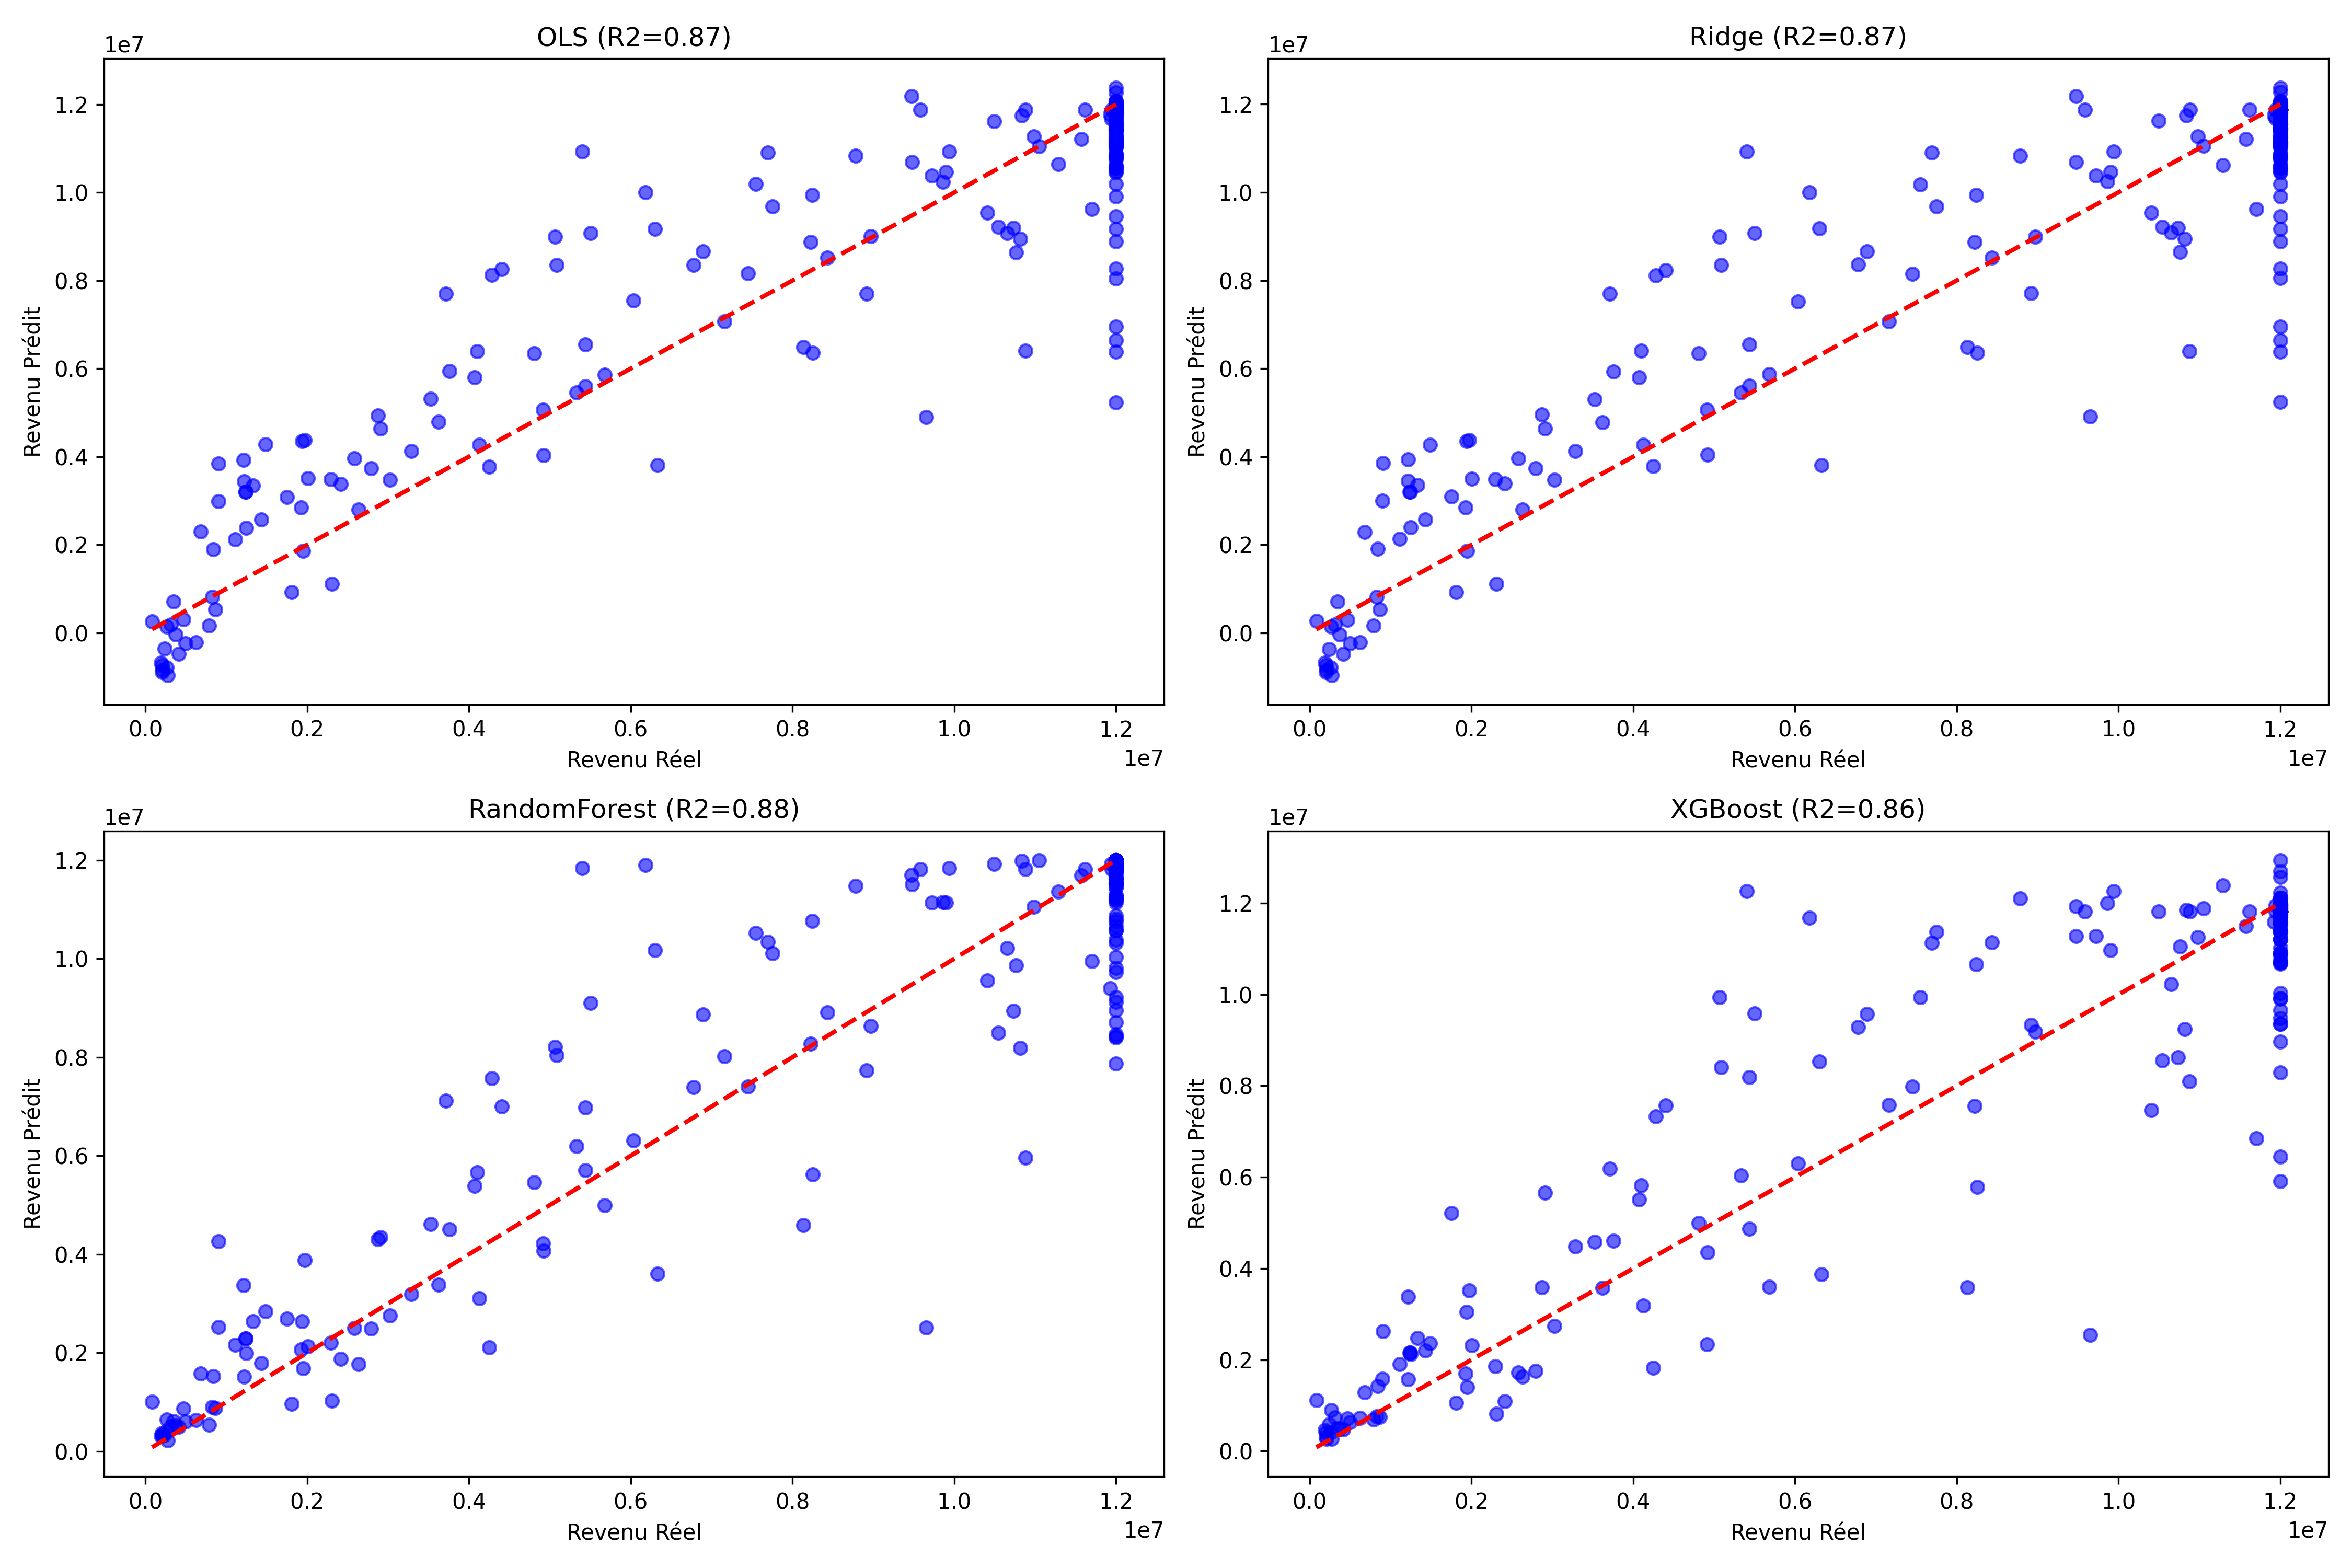
\includegraphics[width=\textwidth]{figures/regression_benchmark.png}
    \caption{Nuages de points (Actual vs Predicted) pour les 4 modèles de régression.}
    \vspace{0.2cm}
    \begin{minipage}{\textwidth}
    \textbf{Description :} Cette grille de graphiques compare visuellement les performances des quatre algorithmes de régression testés (OLS, Ridge, Random Forest, XGBoost). L'axe horizontal représente les revenus réels observés tandis que l'axe vertical représente les prédictions des modèles. Plus les points se concentrent le long de la diagonale, plus le modèle est précis. On y observe clairement la supériorité des modèles arborescents pour capter les relations non-linéaires.
    \end{minipage}
    \label{fig:reg_scatter}
\end{figure}

\FloatBarrier

\begin{figure}[h]
    \centering
    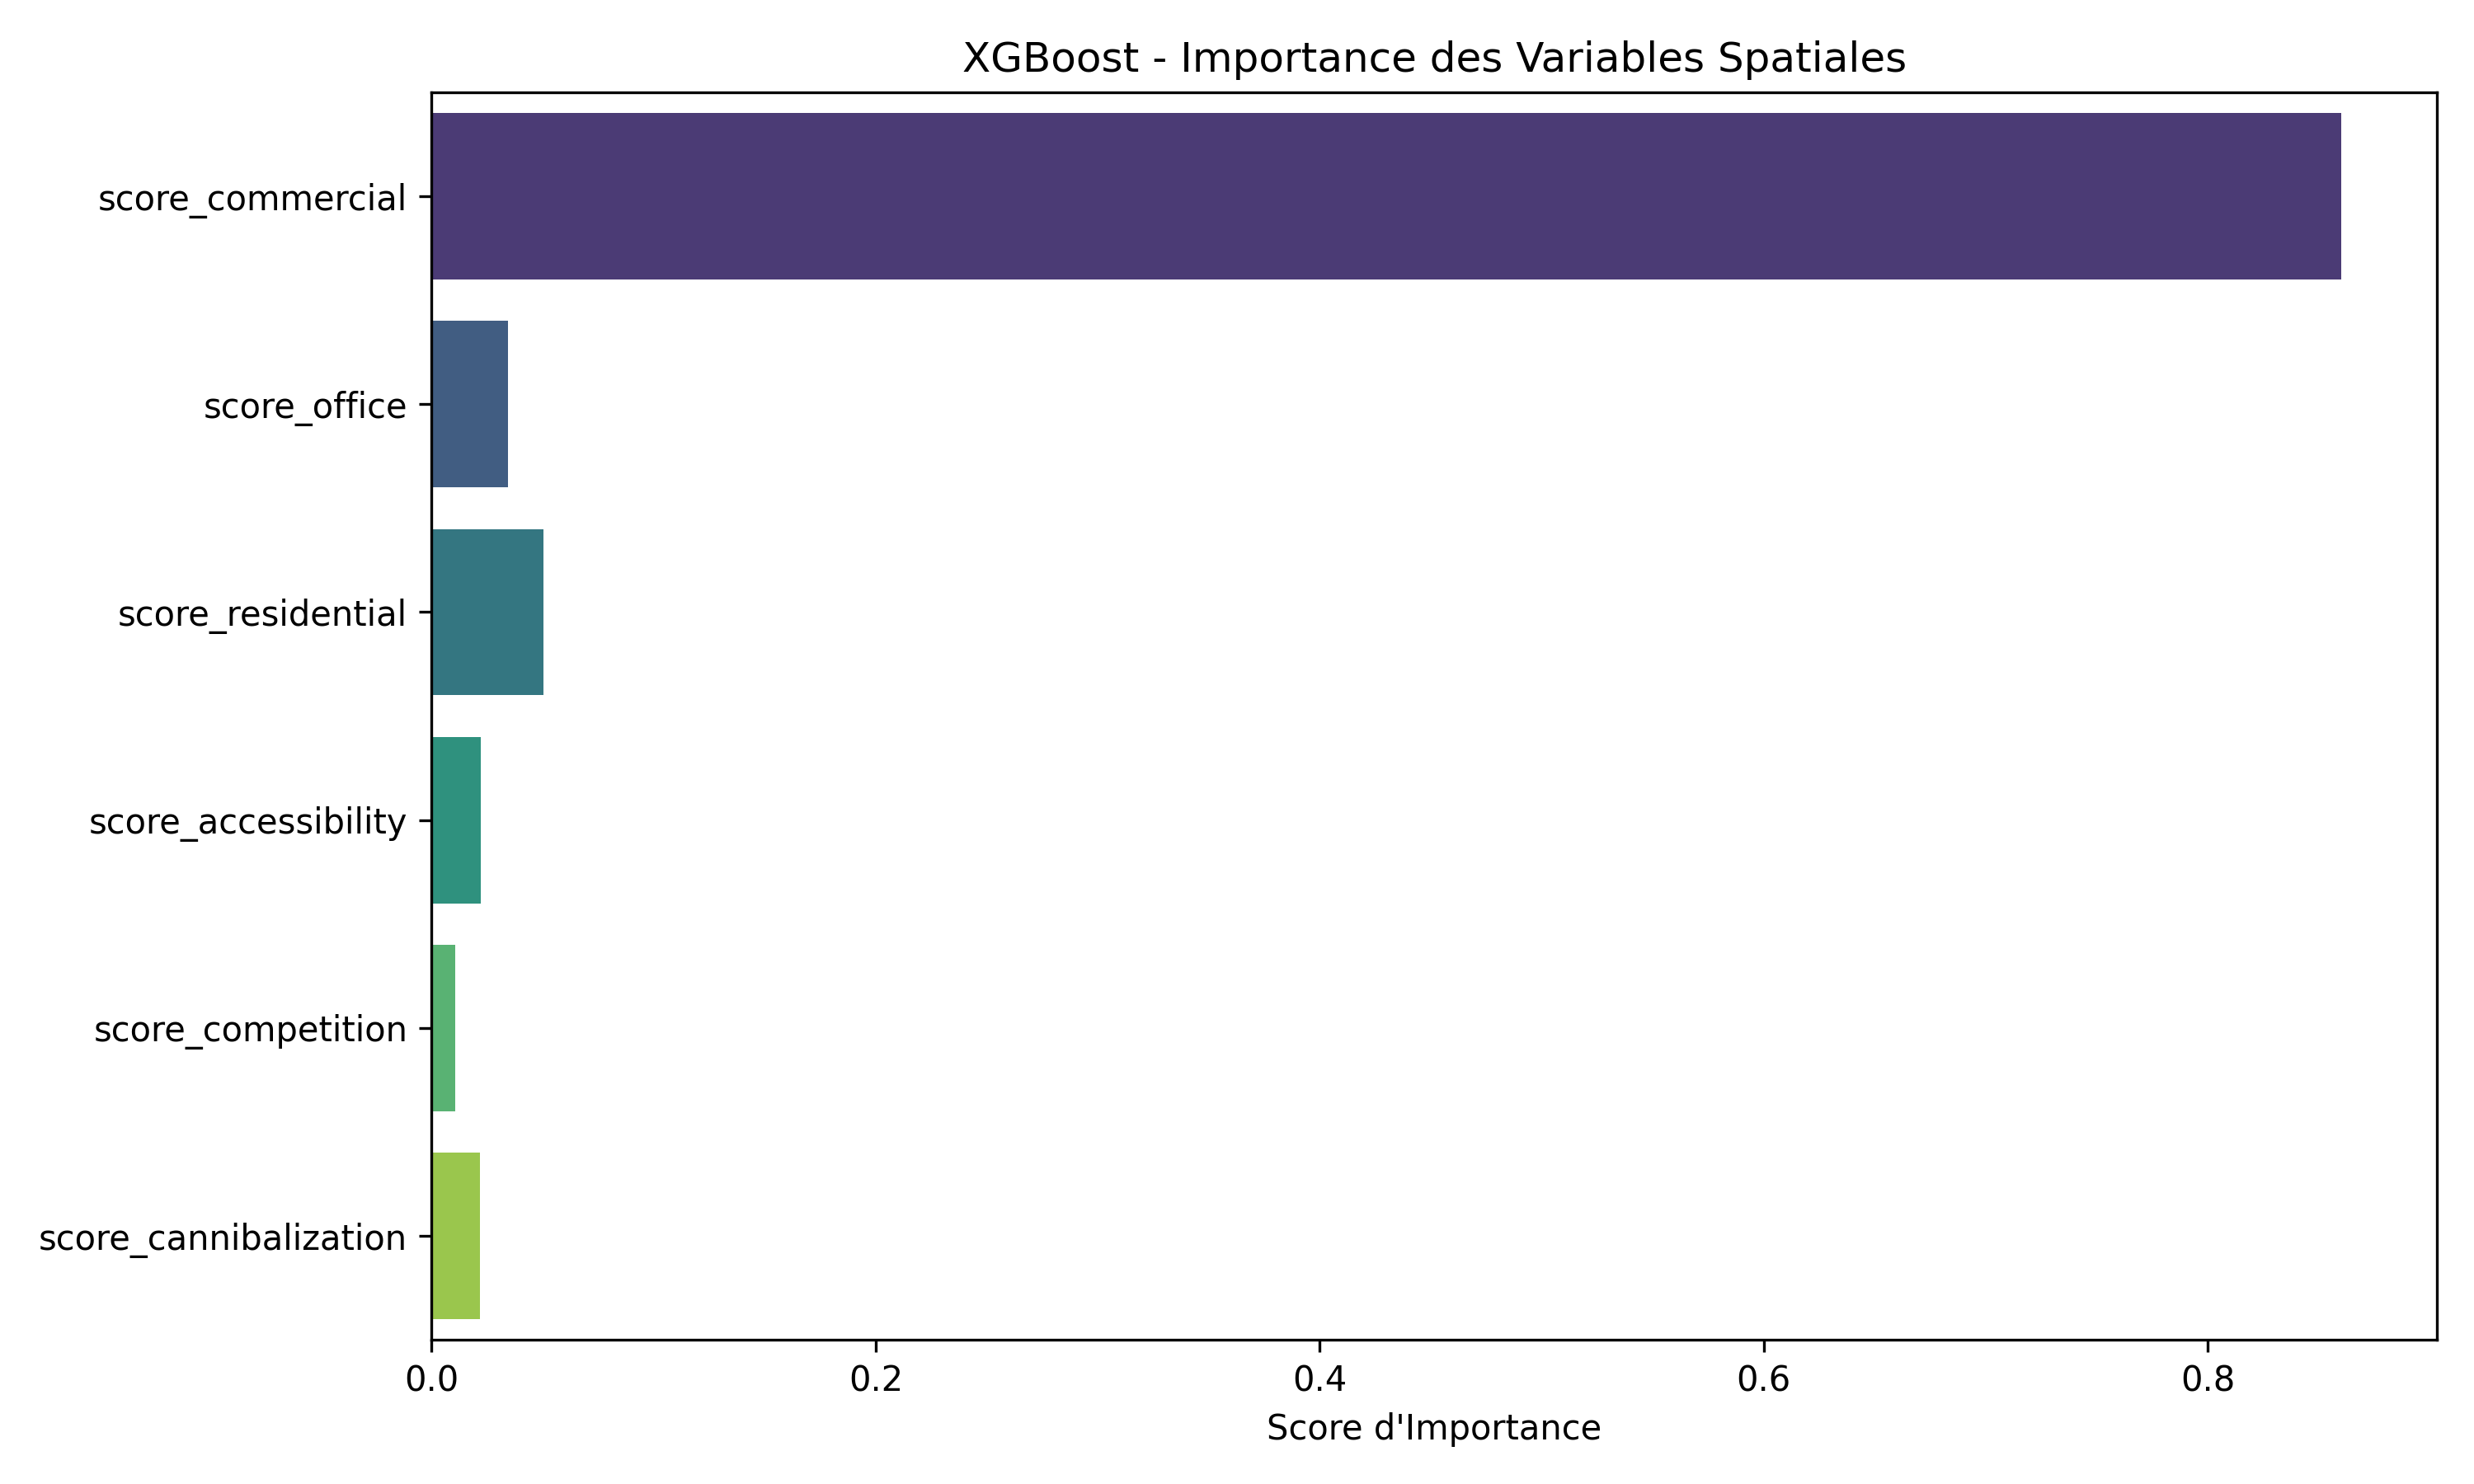
\includegraphics[width=0.6\textwidth]{figures/xgboost_importance.png}
    \caption{Importance des caractéristiques spatiales selon XGBoost (gain moyen).}
    \vspace{0.2cm}
    \begin{minipage}{\textwidth}
    \textbf{Description :} Ce graphique en barres classe les variables d'entrée selon leur niveau de contribution (Gain) au pouvoir prédictif de l'algorithme XGBoost. Il démontre empiriquement que l'attractivité commerciale est de très loin le prédicteur géographique le plus déterminant pour la rentabilité d'une agence, validant ainsi mathématiquement l'intuition métier du secteur bancaire.
    \end{minipage}
    \label{fig:feature_importance}
\end{figure}

\FloatBarrier

\subsection{Benchmarking Algorithmique : Classification Multi-Classes}

En parallèle de la régression, nous avons modélisé le problème sous forme de classification. Chaque agence est assignée à l'une des trois classes d'action stratégique : \textbf{KEEP} (revenu $> 11\,000\,000$ MAD), \textbf{REVIEW} (revenu entre 6\,000\,000 et 11\,000\,000 MAD), ou \textbf{CLOSE} (revenu $< 6\,000\,000$ MAD). Ces seuils reflètent les contraintes opérationnelles de rentabilité du réseau bancaire.

\subsubsection{Modèles Évalués}

Quatre algorithmes de classification ont été entraînés et évalués :
\begin{enumerate}
    \item \textbf{Régression Logistique} \cite{hosmer2013} (\texttt{max\_iter=1000}) : Extension multi-classe du modèle logit via la stratégie One-vs-Rest.
    \item \textbf{K-Nearest Neighbors} \cite{cover1967} ($K=5$) : Classification par vote majoritaire des 5 plus proches voisins dans l'espace standardisé.
    \item \textbf{Random Forest Classifier} ($B=100$) : Forêt aléatoire adaptée à la classification par vote d'arbres.
    \item \textbf{XGBoost Classifier} ($T=100$, $d=4$) : Gradient boosting avec fonction de perte \textit{multi:softmax}.
\end{enumerate}

\subsubsection{Résultats et Matrices de Confusion}

\begin{table}[h]
\centering
\begin{tabular}{|l|c|}
\hline
\textbf{Modèle} & \textbf{Accuracy} \\ \hline
Régression Logistique & 82.92\% \\ \hline
K-Nearest Neighbors & 81.25\% \\ \hline
Random Forest Classifier & 81.67\% \\ \hline
XGBoost Classifier & 82.08\% \\ \hline
\end{tabular}
\caption{Précision globale (Accuracy) des 4 modèles de classification multi-classes.}
\label{tab:clf_benchmark}
\end{table}

L'analyse des matrices de confusion (figure~\ref{fig:confusion_matrices}) révèle que l'ensemble des modèles présentent une précision globale supérieure à 81\%, avec la Régression Logistique en tête à \textbf{82.92\%}. Les erreurs de classification se concentrent principalement sur la classe \texttt{REVIEW}, zone de transition naturelle entre les deux extrêmes. Les classes \texttt{KEEP} et \texttt{CLOSE}, plus polarisées, sont identifiées avec une fiabilité supérieure.

\begin{figure}[h]
    \centering
    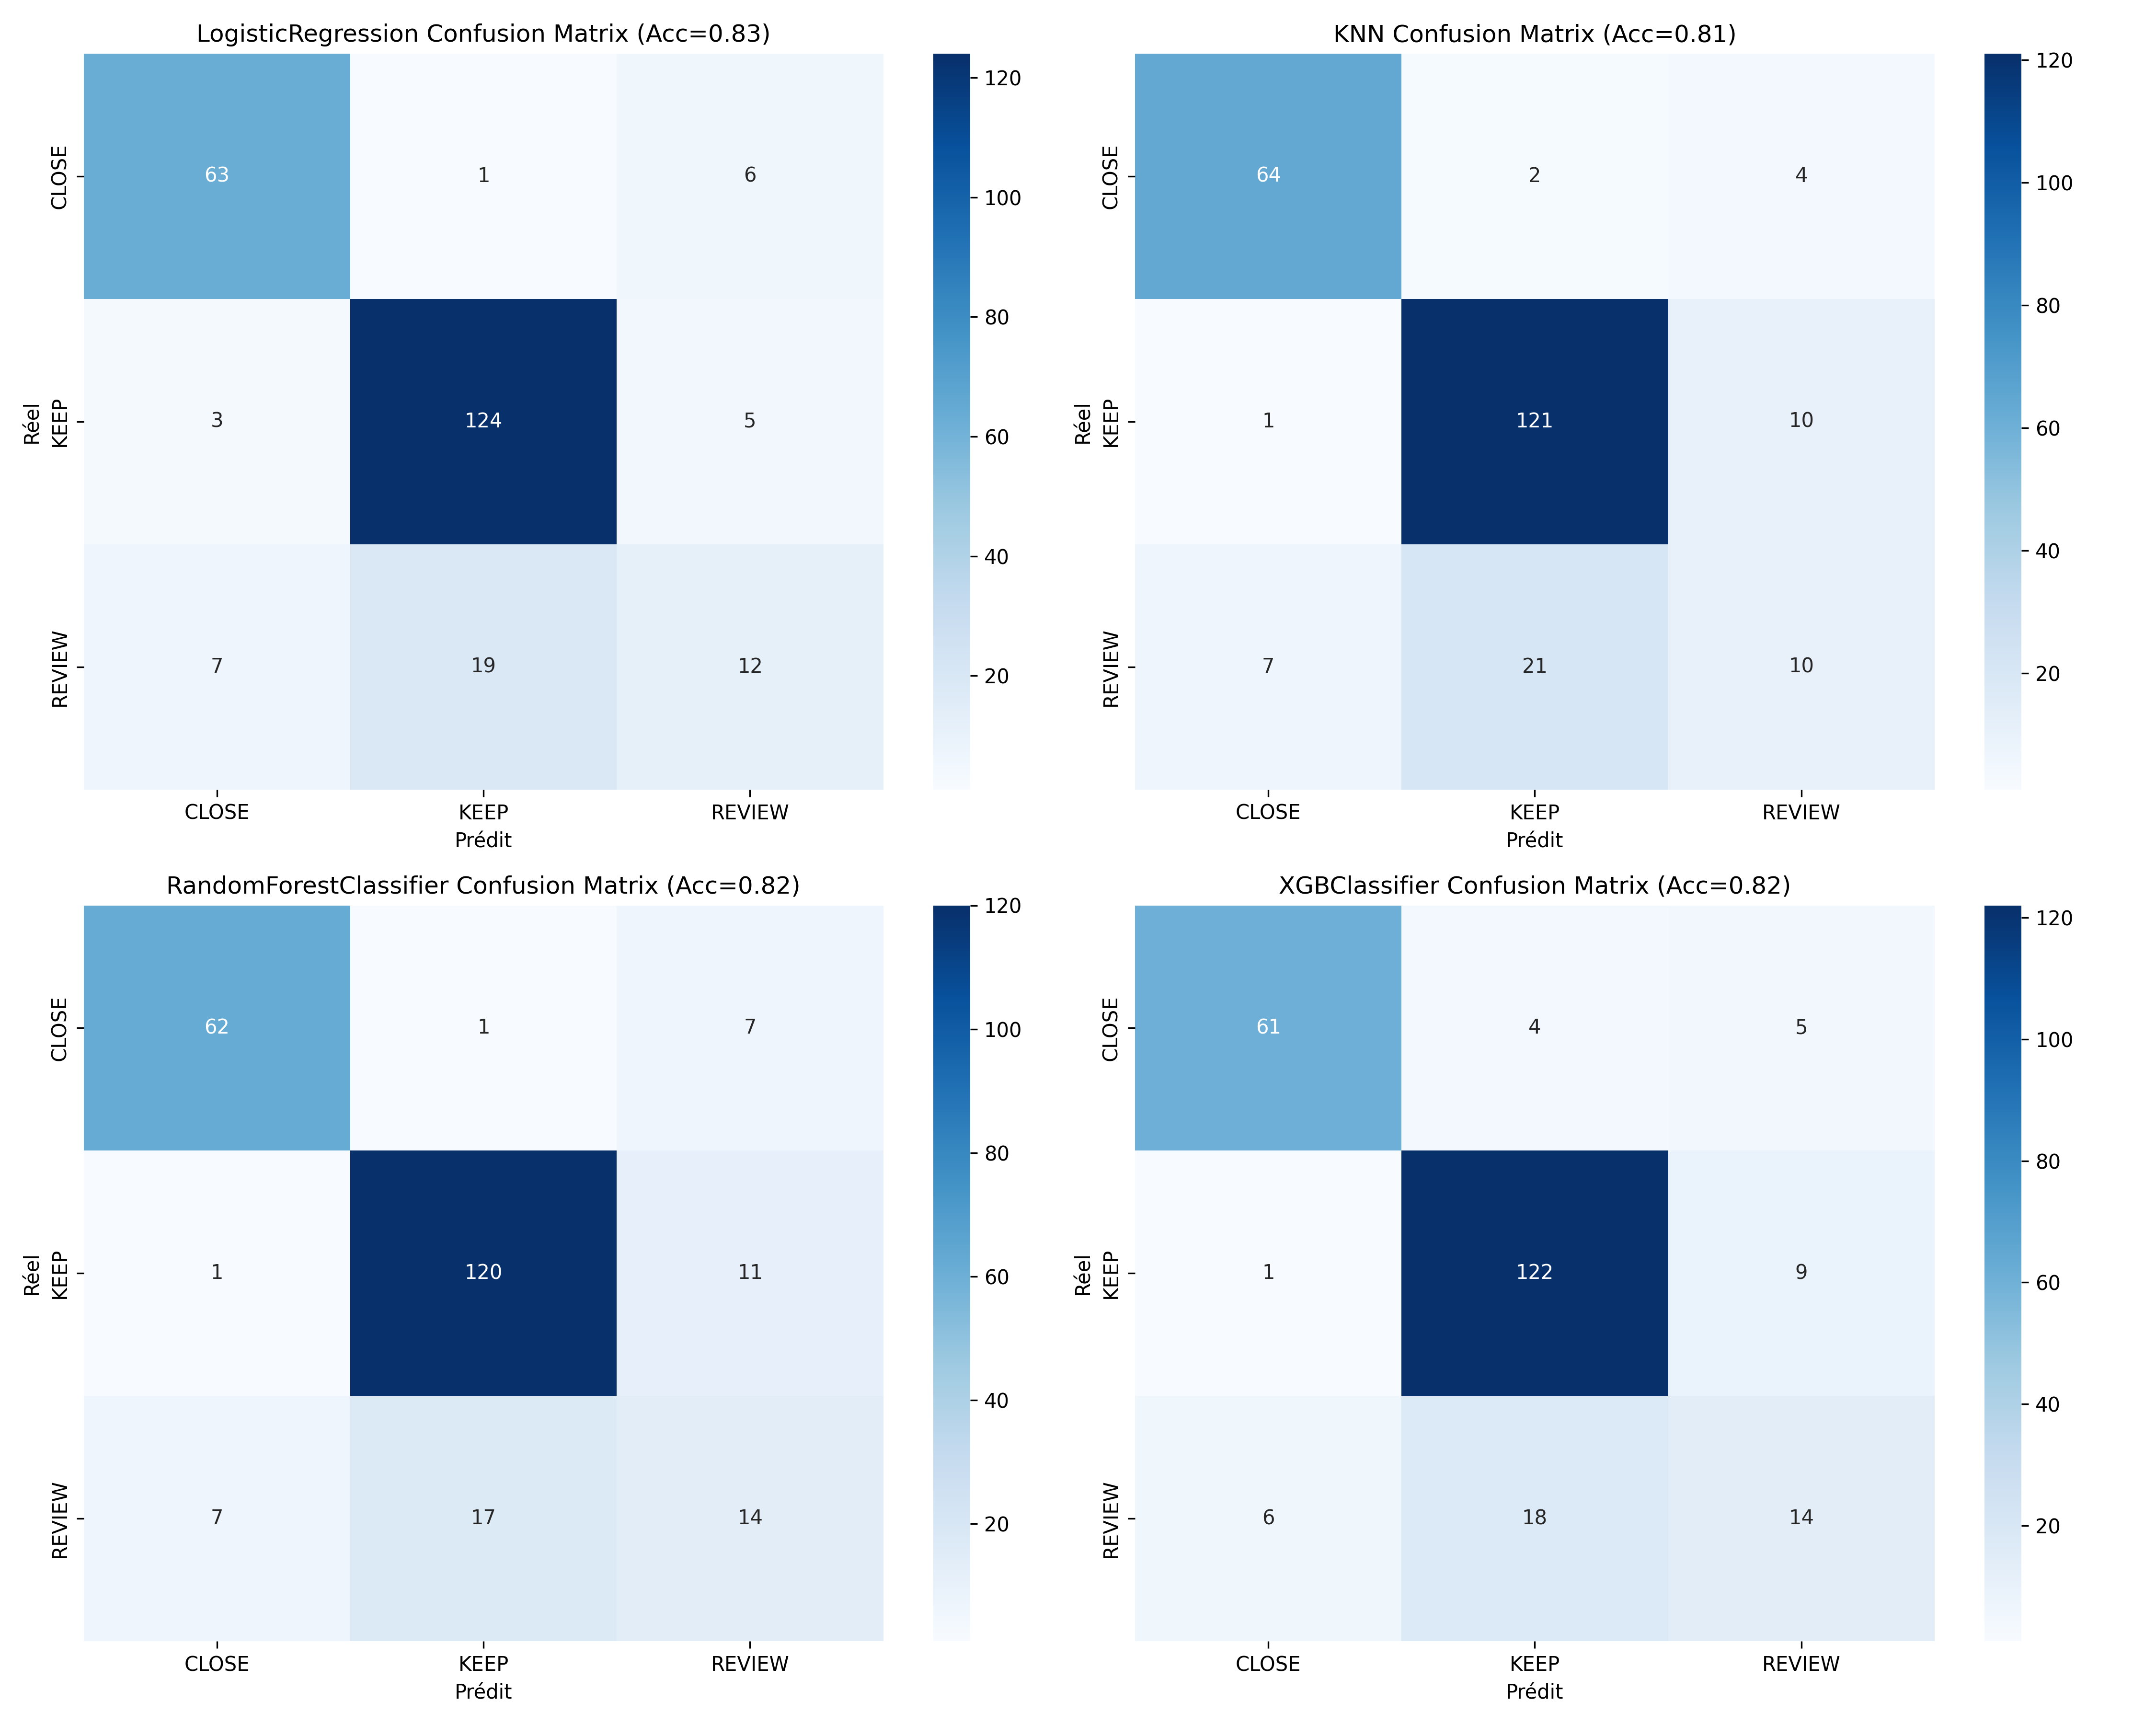
\includegraphics[width=\textwidth]{figures/classification_benchmark.png}
    \caption{Matrices de confusion des 4 modèles de classification.}
    \vspace{0.2cm}
    \begin{minipage}{\textwidth}
    \textbf{Description :} Ces grilles d'évaluation détaillent les performances de nos quatre modèles (Régression Logistique, KNN, Random Forest, XGBoost) lorsqu'ils sont appliqués à la classification des agences en trois actions stratégiques (KEEP, REVIEW, CLOSE). Les matrices permettent d'analyser la répartition exacte des vrais positifs, faux positifs et faux négatifs, montrant que les modèles identifient fiablement les cas extrêmes mais rencontrent des difficultés sur la classe de transition.
    \end{minipage}
    \label{fig:confusion_matrices}
\end{figure}

\FloatBarrier

\subsection{La Matrice BCG Spatiale et l'Analyse des Écarts (Gap Analysis)}

La finalité de l'UC1 n'est pas simplement d'obtenir un modèle de prédiction performant, mais d'exploiter les \textit{résidus} du modèle comme outil de diagnostic stratégique. C'est le principe de la \textbf{Gap Analysis} (Analyse des Écarts).

\subsubsection{Principe Fondamental}

Soit $\hat{Y}_i$ le revenu potentiel prédit par XGBoost (reflétant exclusivement la qualité géographique de l'emplacement) et $Y_i$ le revenu réel observé (reflétant la combinaison emplacement + management). L'espace bidimensionnel $(X = \hat{Y}_i, Y = Y_i)$ constitue notre Matrice BCG adaptée au secteur bancaire.

\subsubsection{Lignes de Potentiel et Définition des Quadrants}

Le plan est divisé par deux lignes critiques dont l'intersection crée quatre quadrants stratégiques :
\begin{enumerate}
    \item \textbf{La médiane des prédictions (Ligne Verticale)} : sépare les zones géographiquement pauvres (à gauche) des zones riches en potentiel (à droite). Calculée à la valeur médiane des sorties XGBoost.
    \item \textbf{La médiane des revenus réels (Ligne Horizontale)} : sépare les agences en sous-performance brute (en bas) des agences très rentables (en haut).
\end{enumerate}

Les quatre quadrants résultants sont :
\begin{itemize}
    \item \textbf{FLAGSHIP (Haut-Droite)} : 514 agences (43\%). Potentiel élevé ET performance élevée. Les agences modèles du réseau.
    \item \textbf{REVIEW / INVEST (Bas-Droite)} : 86 agences (7.2\%). Anomalie critique : le quartier est excellent mais l'agence sous-performe. Action de management, d'audit ou de refonte marketing prioritaire.
    \item \textbf{MONITOR (Haut-Gauche)} : 85 agences (7.1\%). Le quartier a un faible potentiel, mais l'équipe surperforme. Félicitation sans investissement lourd.
    \item \textbf{CLOSE (Bas-Gauche)} : 511 agences (42.7\%). Potentiel inexistant et revenus catastrophiques. Cibles premières d'un plan de fermeture ou de délocalisation.
\end{itemize}

\subsubsection{La Ligne d'Espérance de Potentiel (Diagonale $y = x$)}

L'élément analytique le plus puissant de la matrice est la \textbf{diagonale parfaite} définie par $y = x$, où le revenu réel égale exactement le revenu prédit. Cette ligne représente l'\textit{Espérance de Potentiel} : si une agence se situe sur cette diagonale, sa rentabilité est parfaitement alignée avec le potentiel de son emplacement. Le travail managérial correspond à 100\% aux attentes du modèle.

Toute déviation au-dessus de la diagonale ($Y_i > \hat{Y}_i$) caractérise une \textit{sur-performance} : l'équipe crée de la valeur au-delà de ce que la localisation permettrait naturellement. Inversement, une position sous la diagonale ($Y_i < \hat{Y}_i$) signale une \textit{destruction de valeur} latente.

\begin{figure}[h]
    \centering
    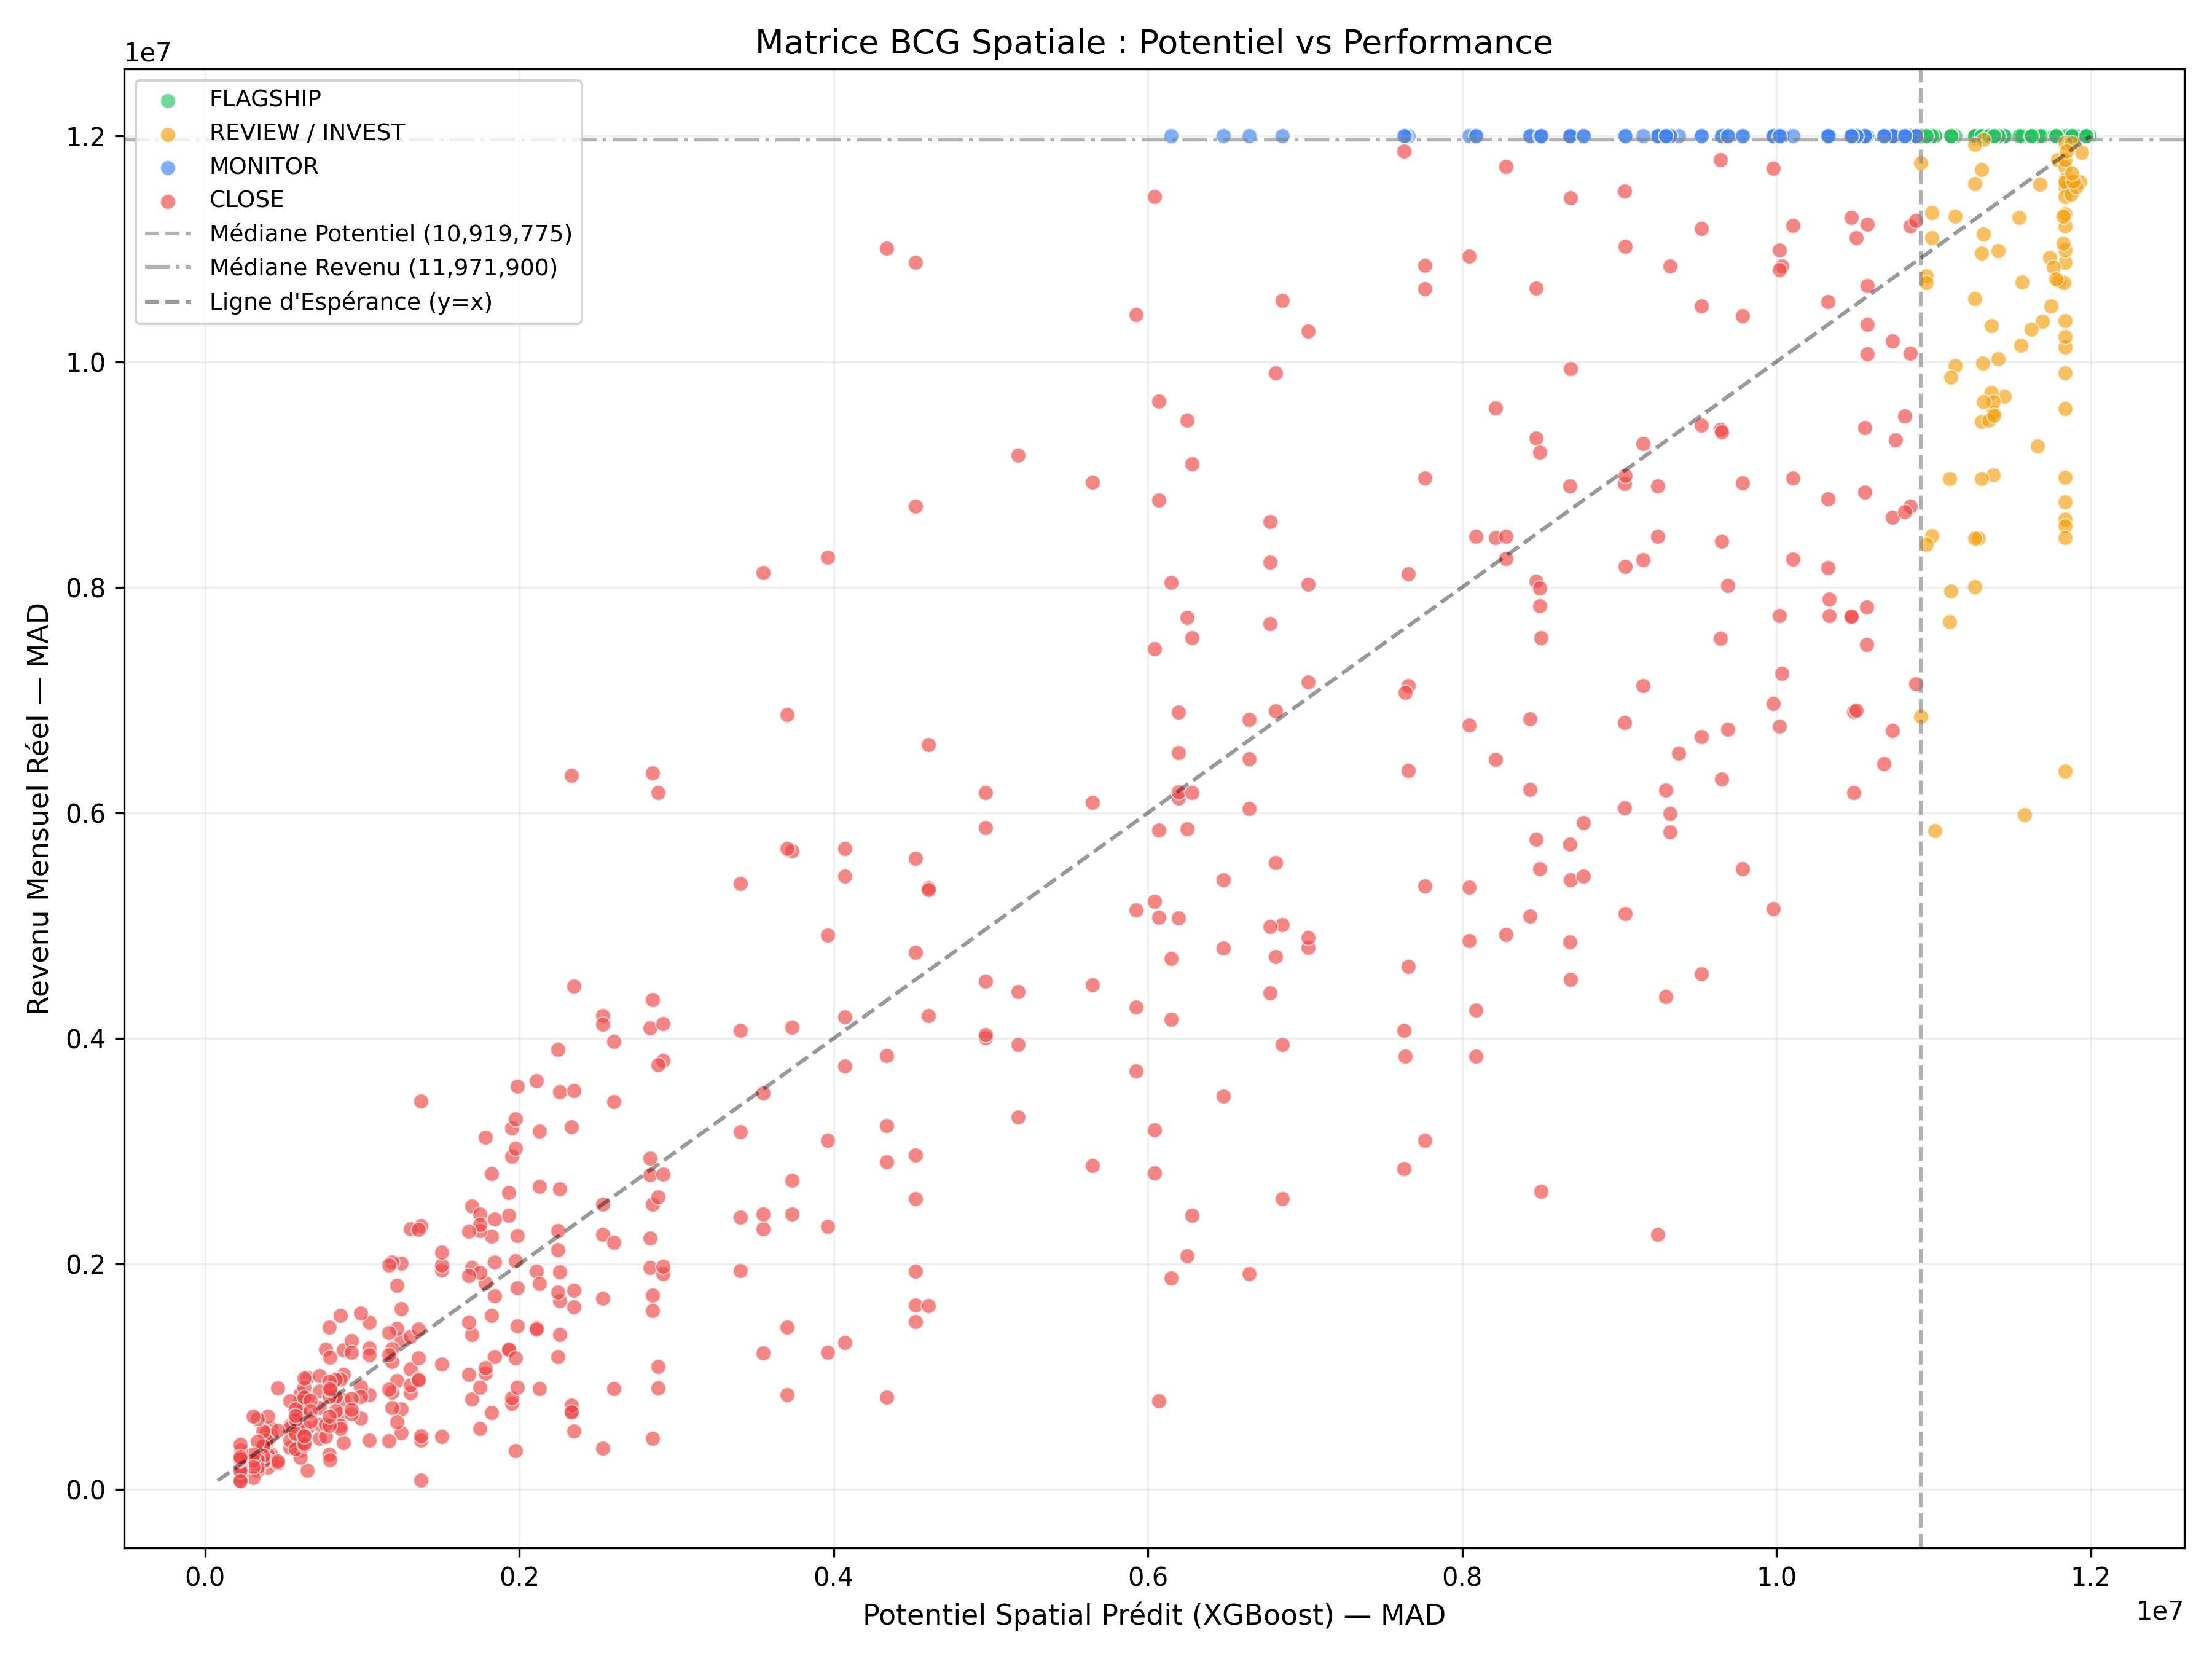
\includegraphics[width=0.85\textwidth]{figures/bcg_matrix.png}
    \caption{Matrice BCG Spatiale}
    \vspace{0.2cm}
    \begin{minipage}{\textwidth}
    \textbf{Description :} Cette matrice est l'outil stratégique central de la Gap Analysis. Chaque point représente une agence physique du réseau. L'axe X illustre le potentiel théorique prédit par le modèle XGBoost basé sur l'emplacement, et l'axe Y montre le revenu réel généré par l'équipe. Les lignes médianes délimitent quatre quadrants d'action (Flagship, Review, Monitor, Close). Enfin, la diagonale noire ($y=x$) représente la ligne d'espérance de potentiel : toute agence située au-dessus surperforme, et toute agence en dessous détruit de la valeur par rapport à son emplacement.
    \end{minipage}
    \label{fig:bcg_matrix}
\end{figure}

\FloatBarrier

\subsection{Optimisation par Fusion : Détection de Cannibalisation via cKDTree}

En complément de l'analyse financière, le système optimise le réseau par la détection des redondances physiques. Deux agences situées à moins de 1.2 km l'une de l'autre se cannibalisent mutuellement en se disputant le même bassin de clientèle.

L'évaluation naïve de toutes les paires de distances entre $N$ agences présente une complexité de $O(N^2)$, inadaptée pour une interface temps réel. Nous avons implémenté l'algorithme des Arbres k-dimensionnels via \texttt{scipy.spatial.cKDTree} (implémenté en C++). L'arbre partitionne l'espace $\mathbb{R}^2$ récursivement via des hyperplans. La fonction \texttt{query\_pairs(r=0.012)} (où 0.012 degrés $\approx$ 1.2 km) exploite l'élagage spatial (\textit{pruning}) pour identifier instantanément les paires cannibales en $O(N \log N)$.

Les paires détectées appartenant aux quadrants REVIEW ou CLOSE de la matrice BCG sont automatiquement proposées comme candidates à une opération de fusion-acquisition interne.

%=============================================================================%
\section{Cas d'Usage 2 : Sélection de Nouveaux Sites (Site Selection)}
%=============================================================================%

Le second cas d'usage se tourne vers la conquête spatiale : identifier les emplacements vierges présentant le plus fort potentiel pour l'ouverture de nouvelles agences.

\subsection{Maillage du Territoire et Filtrage Vectorisé}

L'algorithme génère un maillage de points candidats sur l'étendue des grandes métropoles marocaines (un point tous les 500 mètres). Chaque point virtuel subit le même processus d'agrégation radiale que dans l'UC1, produisant un vecteur spatial $C_j \in \mathbb{R}^6$ identique en structure à celui des agences existantes.

Afin de respecter les contraintes opérationnelles de la banque, un filtrage vectorisé (optimisé via \texttt{pandas}) est appliqué en amont :
\begin{itemize}
    \item Exclusion des zones à densité de population insuffisante (seuil paramétrable).
    \item Exclusion stricte des candidats situés à moins d'une distance $D$ (réglable par l'utilisateur via un slider) d'une agence Attijariwafa existante, appliquant la politique anti-cannibalisation.
    \item Contraintes de diversité géographique par ville (nombre maximum de suggestions par agglomération).
\end{itemize}

\subsection{Sélection par K-NN et Similarité Cosinus}

La sélection finale des meilleurs candidats s'effectue par un algorithme K-Nearest Neighbors utilisant la \textbf{Similarité Cosinus} comme métrique :
\begin{equation}
\text{Sim}(C_j, B_{target}) = \cos(\theta) = \frac{C_j \cdot B_{target}}{||C_j||_2 \cdot ||B_{target}||_2}
\end{equation}
où $B_{target}$ est le centroïde du cluster ``High Performer'' identifié dans l'UC1.

Le choix de la Similarité Cosinus plutôt que la distance Euclidienne est motivé par la \textit{malédiction de la dimensionnalité}. Dans un espace à 6 dimensions, la distance Euclidienne est sensible à la magnitude : une grande zone avec 100 cafés et 50 banques apparaîtrait très éloignée d'une petite zone avec 10 cafés et 5 banques. La Similarité Cosinus mesure l'\textit{angle} entre les vecteurs, identifiant correctement que ces deux zones partagent le même profil commercial (ratio 2:1), indépendamment de leur taille brute.

Les $K=20$ candidats présentant la similarité la plus élevée constituent la recommandation finale pour l'ouverture de nouvelles succursales.

%=============================================================================%
\section{Architecture de Déploiement Logiciel}
%=============================================================================%

L'ensemble de l'intelligence algorithmique (UC1 et UC2) est encapsulé dans une application web monolithique de \textbf{3\,000+ lignes} de code Python, développée avec le framework \texttt{Streamlit}. Ce choix technologique, devenu le standard de l'industrie pour les plateformes d'Internal Tooling en Machine Learning, permet d'exécuter la logique métier (pandas, scikit-learn, XGBoost) et le rendu de l'interface (React) au sein de la même boucle d'exécution.

\subsection{Architecture de l'Interface : Organisation en Onglets}

Le dashboard est structuré en \textbf{11 onglets} thématiques, chacun dédié à une fonctionnalité spécifique :

\begin{table}[h]
\centering
\begin{tabular}{|c|l|l|}
\hline
\textbf{Tab} & \textbf{Nom} & \textbf{Fonction principale} \\ \hline
1 & Map & Carte interactive Folium avec code couleur par action \\ \hline
2 & Rankings & Classement des agences par score composite \\ \hline
3 & ML Clusters & Visualisation PCA des 5 profils K-Means \\ \hline
4 & Mergers & Détection des paires cannibales (cKDTree) \\ \hline
5 & Cities & Analyse macroscopique ville par ville \\ \hline
6 & Deep Dive & Fiche 360° d'audit d'une agence individuelle \\ \hline
7 & Data & Vue tabulaire brute des datasets \\ \hline
8 & Site Selection & Moteur interactif avec sliders et contraintes \\ \hline
9 & Network Optimization & Matrice BCG spatiale et actions stratégiques \\ \hline
10 & Data Enrichment & Scraping live et pipeline de nettoyage \\ \hline
\end{tabular}
\caption{Architecture des 10 onglets du dashboard Branch Intelligence.}
\label{tab:dashboard_tabs}
\end{table}

\subsection{Gestion de la Performance : Cache et État}

Le chargement du dataset principal ($\sim$230 Ko, 1\,198 lignes $\times$ 31 colonnes) est optimisé via le décorateur \texttt{@st.cache\_data}. Ce mécanisme de memoization assure que le fichier CSV n'est parsé qu'une seule fois au démarrage du serveur, les appels suivants retournant directement la copie en mémoire vive. L'état inter-interactions est géré via \texttt{st.session\_state}, un dictionnaire persistant entre les re-rendus de Streamlit.

\subsection{Module d'Enrichissement Asynchrone (Tab 11)}

Le défi architectural principal réside dans l'intégration du scraper Google Maps au sein du dashboard sans bloquer le thread principal de Streamlit. L'architecture implémentée repose sur un paradigme producteur-consommateur :

\begin{enumerate}
    \item \textbf{Producteur (Processus Enfant)} : Le scraper est lancé via \texttt{subprocess.Popen} avec une variable d'environnement \texttt{PYTHONIOENCODING=utf-8} injectée pour assurer la compatibilité des caractères Unicode dans le pipe Windows.
    \item \textbf{Tampon (Thread d'Arrière-Plan)} : Un \texttt{threading.Thread} daemon lit continuellement le flux \texttt{stdout} du processus enfant et pousse chaque ligne dans une \texttt{queue.Queue} thread-safe.
    \item \textbf{Consommateur (Boucle UI)} : La boucle principale de Streamlit vide la queue toutes les 500ms, nettoie les codes ANSI (colorama) via une expression régulière, et met à jour un composant \texttt{st.empty()} pour un rendu temps réel.
\end{enumerate}

Cette architecture producteur-consommateur permet à l'utilisateur d'observer le scraping en direct, puis de déclencher séquentiellement \texttt{clean.py} et \texttt{cleanall.py} pour intégrer les nouvelles données au pipeline d'analyse, créant ainsi une plateforme \textit{End-to-End} totalement auto-suffisante.




\chapter{Réalisation de la Solution}

\section{Introduction}

Ce cinquième chapitre présente la réalisation concrète de la plateforme \textit{Branch Intelligence}. Après avoir défini les fondements théoriques (Chapitre 3) et détaillé l'implémentation algorithmique (Chapitre 4), nous décrivons ici l'application web interactive qui constitue le livrable final du projet. Cette application transforme les modèles de Machine Learning et les algorithmes spatiaux en un outil d'aide à la décision directement exploitable par les décideurs d'Attijariwafa Bank, sans aucune compétence technique requise de leur part.

L'application se distingue par son architecture monolithique unifiée : l'ensemble du pipeline --- de l'acquisition des données brutes jusqu'à la recommandation stratégique finale --- est encapsulé dans un seul point d'entrée, offrant une expérience utilisateur fluide et cohérente.

\section{Outils et Technologies Utilisés}

La réalisation de la solution repose sur un écosystème technologique Python riche et mature, sélectionné pour sa robustesse, sa compatibilité et son adoption massive dans l'industrie du Machine Learning.

\subsection{Streamlit — Framework d'Interface Web}

\texttt{Streamlit} \cite{streamlit} (version 1.x) est un framework Python open-source développé par Snowflake, devenu le standard de l'industrie pour le déploiement rapide d'applications de Data Science. Contrairement aux frameworks web classiques (Django, Flask) qui exigent la construction séparée d'un backend API et d'un frontend JavaScript, Streamlit permet de générer une interface web interactive complète en Python pur.

\textbf{Justification du choix :} Notre application intègre directement des modèles scikit-learn, XGBoost et des structures spatiales cKDTree dans la boucle de rendu. Streamlit est le seul framework permettant cette intégration native sans couche d'abstraction API, réduisant drastiquement le temps de développement et la complexité architecturale.

\textbf{Fonctionnalités exploitées :}
\begin{itemize}
    \item \texttt{st.tabs()} : Organisation de l'interface en 10 onglets thématiques.
    \item \texttt{@st.cache\_data} : Mémoisation du chargement CSV pour des performances instantanées.
    \item \texttt{st.session\_state} : Persistance de l'état utilisateur entre les interactions.
    \item \texttt{st.columns()}, \texttt{st.metric()} : Mise en page responsive avec KPIs visuels.
    \item \texttt{st.plotly\_chart()} : Intégration native des graphiques interactifs.
\end{itemize}

\subsection{Folium — Cartographie Interactive}

\texttt{Folium} \cite{folium} est une bibliothèque Python qui génère des cartes interactives basées sur \texttt{Leaflet.js}. Dans notre application, Folium est utilisé pour le rendu géospatial de la carte principale (Tab 1), affichant les 1\,198 agences avec un code couleur correspondant à leur action stratégique recommandée (KEEP, REVIEW, CLOSE). Chaque marqueur est enrichi d'un popup HTML contenant le nom de l'agence, son score composite, son cluster K-Means et son action.

\subsection{Plotly — Visualisation Interactive Avancée}

\texttt{Plotly} \cite{plotly} est la bibliothèque de visualisation principale de l'application. Contrairement à Matplotlib (statique), Plotly génère des graphiques interactifs permettant le zoom, le survol (hover tooltips), et l'export PNG. Les types de graphiques exploités incluent :
\begin{itemize}
    \item \texttt{Scatter} : Nuages de points pour la Matrice BCG et les projections PCA.
    \item \texttt{Bar} : Classements horizontaux des agences et comparaisons par ville.
    \item \texttt{Indicator / Gauge} : Jauges circulaires pour le score composite dans le module Deep Dive.
    \item \texttt{Heatmap} : Matrices de corrélation et diagrammes radar pour le profilage des clusters.
    \item \texttt{Choropleth / ScatterMapbox} : Cartes géographiques intégrées pour le module Site Selection.
\end{itemize}

\subsection{Scikit-learn — Pipeline de Machine Learning}

\texttt{Scikit-learn} \cite{scikit2011} fournit l'infrastructure complète du pipeline ML :
\begin{itemize}
    \item \texttt{StandardScaler} : Normalisation Z-Score préalable au clustering.
    \item \texttt{KMeans} ($K=5$, $n\_init=10$) : Segmentation non supervisée du réseau.
    \item \texttt{DBSCAN} : Détection de zones denses organiques.
    \item \texttt{PCA} : Réduction de dimensionnalité pour la visualisation 2D/3D des clusters.
\end{itemize}

\subsection{XGBoost — Modèle de Prédiction}

\texttt{XGBoost} (eXtreme Gradient Boosting) est utilisé dans le module Network Optimization (Tab 9) pour la prédiction des revenus basée sur les caractéristiques spatiales. Le modèle entraîné en temps réel dans le dashboard (\texttt{xgb.XGBRegressor(n\_estimators=100)}) produit les prédictions qui alimentent la matrice BCG.

\subsection{SciPy — Algorithmique Spatiale}

Le module \texttt{scipy.spatial.cKDTree} (implémenté en C++) est le moteur d'indexation spatiale de l'application. Il est utilisé dans trois contextes critiques :
\begin{itemize}
    \item Détection des fusions (Tab 4 - Mergers) via \texttt{query\_pairs(r=0.012)}.
    \item Enrichissement des candidats en densité de population (Tab 8 - Run Site Selection).
    \item Identification des agences proches dans le module d'optimisation réseau (Tab 9).
\end{itemize}

\subsection{Selenium WebDriver — Scraping Dynamique}

\texttt{Selenium} pilote un navigateur Chrome en mode \textit{headless} pour le scraping Google Maps. L'intégration dans le dashboard (Tab 10) utilise \texttt{subprocess.Popen} et \texttt{threading.Thread} pour une exécution asynchrone non-bloquante.

\subsection{Pandas et NumPy — Manipulation des Données}

\texttt{Pandas} constitue l'épine dorsale de toutes les transformations de données : chargement CSV, filtrage vectorisé, agrégation par groupe (\texttt{groupby}), et jointures. \texttt{NumPy} fournit les opérations matricielles sous-jacentes pour les calculs de distance et de similarité cosinus.

\subsection{Synthèse de l'Environnement Technique}

\begin{table}[h]
\centering
\begin{tabular}{|l|l|l|}
\hline
\textbf{Catégorie} & \textbf{Technologie} & \textbf{Usage} \\ \hline
Interface Web & Streamlit & Framework principal du dashboard \\ \hline
Cartographie & Folium + Leaflet.js & Carte interactive (Tab 1) \\ \hline
Visualisation & Plotly & Graphiques interactifs (10 tabs) \\ \hline
Machine Learning & Scikit-learn, XGBoost & K-Means, PCA, Régression \\ \hline
Spatial & SciPy (cKDTree) & Requêtes spatiales $O(N \log N)$ \\ \hline
Scraping & Selenium + Chrome & Acquisition Google Maps \\ \hline
Data & Pandas, NumPy & ETL et calculs matriciels \\ \hline
Langage & Python 3.14 & Langage principal \\ \hline
\end{tabular}
\caption{Synthèse de la stack technologique de la plateforme Branch Intelligence.}
\label{tab:tech_stack}
\end{table}

\section{Architecture de l'Application}

L'application est structurée en \textbf{10 onglets (Tabs)} organisés selon une progression logique : de l'exploration générale vers l'action spécifique. Chaque onglet constitue un module fonctionnel autonome mais interconnecté aux autres via le dataset partagé en mémoire. Les sections suivantes détaillent chaque module.

\subsection{Module 1 — Carte Interactive (Map)}

Le premier onglet constitue le point d'entrée visuel de l'application. Il présente une carte interactive \texttt{Folium} centrée sur le Maroc, sur laquelle les 1\,196 agences sont représentées par des marqueurs circulaires dont la couleur encode l'action stratégique recommandée :

\begin{itemize}
    \item \textbf{Vert} (\texttt{\#22C55E}) : KEEP — Invest (agences performantes à maintenir).
    \item \textbf{Vert clair} (\texttt{\#86EFAC}) : KEEP — Flagship (performantes mais proches d'une autre agence).
    \item \textbf{Jaune} (\texttt{\#EAB308}) : REVIEW — À auditer.
    \item \textbf{Orange} (\texttt{\#F97316}) : REVIEW — Candidate à une fusion.
    \item \textbf{Rouge} (\texttt{\#EF4444}) : CLOSE — Redondante.
    \item \textbf{Rouge foncé} (\texttt{\#991B1B}) : CLOSE — Sous-performante.
\end{itemize}

Chaque marqueur est enrichi d'un popup HTML affichant : le nom de l'agence, le score composite, le cluster K-Means, et l'action recommandée. Un panneau latéral permet de filtrer par ville, par cluster, et par plage de score composite.

\begin{figure}[h]
    \centering
    \includegraphics[width=0.68\textwidth]{screenshot_map.png}
    \caption{Module Map --- Vue d'ensemble du réseau bancaire national.}
    \label{fig:screenshot_map}
\end{figure}

\FloatBarrier

Chaque marqueur représente une agence, coloré selon l'action stratégique recommandée : vert (KEEP), jaune (REVIEW), rouge (CLOSE). Le survol d'un marqueur affiche un popup HTML avec le nom, le score composite, le cluster K-Means et l'action. Le panneau latéral permet de filtrer par ville, cluster et plage de score.

\subsection{Module 2 — Classements (Rankings)}

Ce module présente les agences sous forme de classements tabulaires dynamiques. L'utilisateur peut trier par score composite (Top 20, Bottom 20), par ville, ou par action. Un graphique à barres horizontales Plotly accompagne le tableau, permettant une lecture visuelle immédiate de la hiérarchie du réseau.

Trois KPIs sont affichés en en-tête :
\begin{itemize}
    \item Nombre d'agences à conserver (KEEP).
    \item Nombre d'agences à fermer (CLOSE).
    \item Score composite moyen du réseau.
\end{itemize}

\begin{figure}[h]
    \centering
    \includegraphics[width=0.8\textwidth]{screenshot_rankings_top.png}
    \caption{Module Rankings --- Classement des agences par score composite.}
    \label{fig:screenshot_rankings_top}
\end{figure}

\FloatBarrier

En haut, trois métriques KPI résument l'état du réseau (nombre d'agences KEEP, CLOSE, et score moyen). En dessous, un graphique à barres horizontales Plotly classe les 20 meilleures agences par score composite décroissant, permettant d'identifier immédiatement les points forts du réseau.

\subsection{Module 3 — Clusters ML}

Ce module exploite directement les résultats du clustering K-Means ($K=5$) et de la projection PCA présentés au Chapitre 4. L'interface se compose de :

\begin{enumerate}
    \item \textbf{Scatter Plot PCA 2D :} Projection des agences dans l'espace des deux premières composantes principales (72.5\% + 10.1\% de variance), colorées par cluster. L'utilisateur peut survoler chaque point pour obtenir les détails de l'agence.
    \item \textbf{Radar Charts par Cluster :} Diagrammes radar affichant la signature spatiale moyenne de chaque profil (Commercial, Office, Residential, Accessibility, Competition, Cannibalization).
    \item \textbf{Répartition par Cluster :} Diagramme en barres montrant le nombre d'agences dans chaque profil.
\end{enumerate}

\begin{figure}[h]
    \centering
    \includegraphics[width=0.8\textwidth]{screenshot_clusters_pca.png}
    \caption{Module ML Clusters --- Projection PCA bidimensionnelle des agences.}
    \label{fig:screenshot_clusters_pca}
\end{figure}

\FloatBarrier

Les 1\,198 agences sont projetées dans l'espace des deux premières composantes principales (72.5\% et 10.1\% de variance). Chaque point est coloré selon son cluster K-Means (High Performer, Commercial Hub, Residential Anchor, Underperformer, At Risk). Les diagrammes radar en dessous détaillent la signature spatiale moyenne de chaque profil.

\subsection{Module 4 — Fusions (Mergers)}

Ce module implémente la détection automatique de cannibalisation inter-agences. L'algorithme \texttt{cKDTree} identifie toutes les paires d'agences situées à moins de 1.2 km l'une de l'autre. Pour chaque paire détectée, le module affiche :

\begin{itemize}
    \item Les noms et scores composites des deux agences.
    \item La distance exacte séparant les deux points (en km).
    \item L'action recommandée pour chacune : conserver la plus performante, fermer ou fusionner la moins rentable.
\end{itemize}

Le résultat est présenté sous forme de tableau interactif triable et d'une carte Folium dédiée affichant les paires reliées par des lignes rouges, permettant une visualisation géographique immédiate du phénomène de cannibalisation.

\begin{figure}[h]
    \centering
    \includegraphics[width=0.8\textwidth]{screenshot_mergers_map.png}
    \caption{Module Mergers --- Détection de cannibalisation inter-agences.}
    \label{fig:screenshot_mergers_map}
\end{figure}

\FloatBarrier

Les paires d'agences distantes de moins de 1.2 km sont reliées par des segments rouges sur la carte Folium. Le tableau associé liste chaque paire avec les noms, scores composites, distance exacte en km, et la recommandation (conserver la plus performante, fusionner ou fermer la moins rentable).

\subsection{Module 5 — Analyse par Ville (Cities)}

Le module Cities fournit une analyse macroscopique agrégée par agglomération. Pour chaque ville du réseau, le système calcule et affiche :

\begin{itemize}
    \item Le nombre total d'agences dans la ville.
    \item Le score composite moyen, minimum et maximum.
    \item Le score commercial moyen et le score de compétition moyen.
    \item La proportion d'agences classées KEEP vs CLOSE.
\end{itemize}

Un graphique à barres Plotly permet de comparer visuellement les villes entre elles. L'utilisateur peut sélectionner une ville spécifique pour obtenir un zoom détaillé sur ses agences individuelles.

\begin{figure}[h]
    \centering
    \includegraphics[width=0.8\textwidth]{screenshot_cities_chart.png}
    \caption{Module Cities --- Analyse comparative par ville.}
    \label{fig:screenshot_cities_chart}
\end{figure}

\FloatBarrier

Le graphique à barres compare les agglomérations par score composite moyen, nombre d'agences et proportion KEEP vs CLOSE. Un clic sur une ville affiche le détail individuel de chacune de ses agences avec leurs métriques spatiales.

\subsection{Module 6 — Audit Individuel (Deep Dive)}

Ce module constitue la fiche d'identité 360° d'une agence. L'utilisateur sélectionne une agence via un menu déroulant (\texttt{st.selectbox}) et obtient instantanément :

\begin{enumerate}
    \item \textbf{Jauge Composite Score :} Un indicateur Plotly \texttt{Gauge} affichant le score composite avec des zones colorées (rouge $< 0.20$, jaune $0.20-0.35$, vert $> 0.35$) et un delta par rapport à la moyenne du réseau.
    \item \textbf{Scores Détaillés :} Les 6 scores spatiaux individuels présentés sous forme de métriques \texttt{st.metric()} avec indicateurs de tendance.
    \item \textbf{Informations Contextuelles :} Le cluster d'appartenance, l'action recommandée, les coordonnées GPS, et la ville.
    \item \textbf{Carte de Localisation :} Une mini-carte Folium centrée sur l'agence sélectionnée avec un rayon de 1km illustrant la zone d'influence.
\end{enumerate}

\begin{figure}[h]
    \centering
    \includegraphics[width=0.8\textwidth]{screenshot_deepdive_gauge.png}
    \caption{Module Deep Dive --- Fiche d'audit individuelle d'une agence.}
    \label{fig:screenshot_deepdive_gauge}
\end{figure}

\FloatBarrier

La jauge circulaire Plotly affiche le score composite avec des zones colorées (rouge $< 0.20$, jaune $0.20-0.35$, vert $> 0.35$) et un delta par rapport à la moyenne du réseau. Les 6 scores spatiaux individuels sont présentés sous forme de KPI, accompagnés d'une mini-carte Folium centrée sur l'agence avec un cercle de rayon 1 km.

\subsection{Module 7 — Données Brutes (Data)}

Ce module offre une vue transparente sur les données sous-jacentes. Il permet aux analystes de vérifier, filtrer et exporter les datasets utilisés par les algorithmes. Le tableau interactif \texttt{st.dataframe()} supporte le tri par colonne, le filtrage textuel, et la sélection de colonnes à afficher. Les colonnes numériques (comme \texttt{composite\_score}) sont enrichies de barres de progression (\texttt{st.column\_config.ProgressColumn}) pour une lecture visuelle immédiate.

\subsection{Module 8 — Site Selection (Moteur Interactif)}

Ce module constitue le moteur de recommandation de l'application. Il permet à l'utilisateur de paramétrer dynamiquement l'ensemble de la recherche de nouveaux emplacements via une série de contrôles interactifs :

\begin{enumerate}
    \item \textbf{Upload de Données :} L'utilisateur charge son propre fichier CSV de branches scorées et un fichier de données POI fusionnées.
    \item \textbf{Paramètres Spatiaux (Sliders) :}
    \begin{itemize}
        \item Distance minimum aux agences existantes (km) : contrôle anti-cannibalisation.
        \item Rayon d'agrégation POI (km) : taille de la zone d'influence.
        \item Nombre de clusters K-Means : granularité de la segmentation.
        \item Top N candidats à retourner.
    \end{itemize}
    \item \textbf{Pipeline Automatisé :} Au clic du bouton ``Run'', le système exécute séquentiellement :
    \begin{enumerate}
        \item Chargement et validation des données.
        \item Construction du cKDTree pour l'enrichissement en densité de population.
        \item Clustering K-Means et identification du profil ``High Performer''.
        \item Génération de la grille de candidats (un point tous les 500m).
        \item Calcul des scores POI par agrégation radiale via cKDTree.
        \item Filtrage par contraintes (distance minimum, densité, diversité par ville).
        \item Calcul de la similarité cosinus et sélection des Top N.
    \end{enumerate}
    \item \textbf{Visualisation des Résultats :} Les candidats sélectionnés sont affichés sur une carte interactive ScatterMapbox avec tooltips détaillés, accompagnés d'un tableau récapitulatif exportable.
\end{enumerate}

\begin{figure}[h]
    \centering
    \includegraphics[width=0.8\textwidth]{screenshot_runsite_results.png}
    \caption{Module Run Site Selection --- Résultats du moteur de découverte interactif.}
    \label{fig:screenshot_runsite_results}
\end{figure}

\FloatBarrier

Après paramétrage des contraintes (distance minimum, densité, nombre de clusters) via les sliders, le pipeline à 7 étapes s'exécute automatiquement. Les Top N candidats sont affichés sur une carte ScatterMapbox avec tooltips de score, accompagnés d'un tableau récapitulatif exportable en CSV.

\subsection{Module 9 — Optimisation Réseau (Network Optimization)}

Ce module implémente la Matrice BCG Spatiale décrite en détail au Chapitre 4. L'interface se compose de trois sections principales :

\begin{enumerate}
    \item \textbf{Configuration :} L'utilisateur paramètre les seuils de sous-performance et de sur-performance via des sliders. Ces seuils contrôlent la frontière entre les quadrants FLAGSHIP, REVIEW/INVEST, MONITOR et CLOSE.
    \item \textbf{Matrice BCG Interactive :} Un scatter plot Plotly affichant chaque agence dans l'espace (Potentiel Prédit vs Revenu Réel). Les quadrants sont colorés, et le survol d'un point affiche les détails complets de l'agence. Les lignes médianes et la diagonale d'espérance ($y = x$) sont tracées en superposition.
    \item \textbf{Tableau d'Actions :} Un résumé tabulaire des recommandations stratégiques, filtré par quadrant. Les agences REVIEW/INVEST et CLOSE sont mises en évidence avec le détail de leur écart (gap) entre potentiel et performance.
\end{enumerate}

Le module intègre également la détection automatique des agences FLAGSHIP proches d'agences à fermer, suggérant des opportunités de consolidation d'actifs.

\begin{figure}[h]
    \centering
    \includegraphics[width=0.8\textwidth]{screenshot_bcg_scatter.png}
    \caption{Module Network Optimization --- Matrice BCG spatiale interactive.}
    \label{fig:screenshot_bcg_scatter}
\end{figure}

\FloatBarrier

Chaque point représente une agence positionnée dans l'espace (Potentiel Prédit par XGBoost en abscisse, Revenu Réel en ordonnée). Les lignes médianes divisent le plan en 4 quadrants (FLAGSHIP, REVIEW/INVEST, MONITOR, CLOSE). La diagonale noire ($y=x$) représente la ligne d'espérance de potentiel. Le tableau d'actions en dessous liste les recommandations stratégiques filtrées par quadrant.

\subsection{Module 10 — Enrichissement de Données (Data Enrichment)}

Ce dernier module transforme l'application d'un outil d'analyse statique en une plateforme auto-alimentée. Il permet à l'utilisateur de lancer directement le scraper Google Maps depuis l'interface du dashboard.

\textbf{Architecture Technique :} L'onglet implémente un paradigme producteur-consommateur asynchrone :
\begin{itemize}
    \item Le scraper est lancé comme processus enfant via \texttt{subprocess.Popen} avec \texttt{PYTHONIOENCODING=utf-8}.
    \item Un thread daemon lit le \texttt{stdout} en continu et alimente une \texttt{queue.Queue} thread-safe.
    \item La boucle Streamlit vide la queue et affiche la sortie dans un bloc \texttt{st.code()} simulant un terminal en temps réel.
\end{itemize}

\textbf{Contrôles Utilisateur :}
\begin{itemize}
    \item \textbf{Mode de Scraping :} Choix entre ``Reprendre depuis les checkpoints'' ou ``Recommencer à zéro''.
    \item \textbf{Boutons Start/Stop :} Lancement et arrêt gracieux du scraper (les données sont sauvegardées).
    \item \textbf{Console Live :} Affichage en temps réel de la progression exacte du scraper (nombre de POI trouvés, cellule en cours, etc.), reproduisant fidèlement la sortie du terminal.
    \item \textbf{Pipeline Clean \& Merge :} Un bouton dédié exécute séquentiellement \texttt{clean.py} puis \texttt{cleanall.py}, intégrant les nouvelles données dans \texttt{merged\_data\_clean.csv}.
\end{itemize}


\begin{figure}[h]
    \centering
    \includegraphics[width=0.8\textwidth]{screenshot_enrichment.png}
    \caption{Module Data Enrichment --- Interface de scraping Google Maps.}
    \label{fig:screenshot_enrichment}
\end{figure}

\FloatBarrier

L'utilisateur choisit le mode (reprise ou nouveau), lance le scraper via le bouton Start, et observe la progression en temps réel dans une console simulée. Les métriques en haut affichent le nombre d'entrées checkpointées et de POI scrapés. Le bouton Clean \& Merge déclenche séquentiellement le nettoyage et la fusion des données dans le fichier \texttt{merged\_data\_clean.csv}.

\section{Valeur Stratégique et Apport de la Solution}

La plateforme Branch Intelligence apporte une valeur stratégique mesurable à Attijariwafa Bank sur quatre axes :

\subsection{Rationalisation des Décisions d'Investissement}

Avant ce projet, les décisions d'ouverture et de fermeture d'agences reposaient sur l'intuition des directeurs régionaux et des études de marché ponctuelles. La matrice BCG spatiale (Module 9) fournit désormais un cadre quantitatif objectif : les 86 agences identifiées comme REVIEW/INVEST représentent un potentiel de revenus inexploité, tandis que les 513 agences CLOSE constituent des cibles de rationalisation budgétaire.

\subsection{Réduction de la Cannibalisation}

Le module Mergers (Tab 4) a identifié automatiquement les paires d'agences se disputant le même bassin de clientèle. La consolidation de ces doublons permettrait de réduire les coûts opérationnels tout en maintenant la couverture géographique du réseau.

\subsection{Expansion Scientifique du Réseau}

Le moteur de Site Selection (Module 8) remplace les études de faisabilité traditionnelles par un algorithme reproductible et paramétrable. L'utilisation de la similarité cosinus garantit que les nouveaux sites recommandés reproduisent le profil spatial des agences les plus performantes du réseau, maximisant la probabilité de succès commercial. \cite{salton1983}

\subsection{Autonomie Opérationnelle}

Le module Data Enrichment (Tab 10) assure la pérennité du système. L'équipe Analytics peut enrichir la base de données POI de manière autonome, sans intervention de l'équipe de développement, puis relancer les analyses avec des données fraîches. Cette boucle d'auto-alimentation transforme le projet d'un livrable ponctuel en une plateforme vivante.

\chapter*{Conclusion Générale et Perspectives}
\addcontentsline{toc}{chapter}{Conclusion Générale et Perspectives}
\markboth{Conclusion Générale et Perspectives}{Conclusion Générale et Perspectives}

Au terme de ce projet de fin d'études, nous avons abordé la problématique de l'optimisation du réseau d'agences bancaires d'Attijariwafa Bank sous un angle résolument data-driven, en combinant l'analyse géospatiale, l'apprentissage automatique et la visualisation interactive. L'objectif était double : d'une part, évaluer de manière objective la performance territoriale des 1\,196 agences existantes, et d'autre part, proposer un cadre méthodologique rigoureux pour la sélection de nouveaux emplacements à fort potentiel.

La première contribution majeure de ce travail réside dans la construction d'un pipeline de scoring multidimensionnel, qui attribue à chaque agence des indicateurs quantitatifs reflétant la qualité de son environnement immédiat --- zones commerciales, résidentielles, accessibilité, concurrence et densité de population. Ce scoring, combiné à un clustering K-Means en cinq profils (High Performer, Commercial Hub, Residential Anchor, Underperformer, At Risk), offre aux décideurs une cartographie fine et actionnable du réseau.

La seconde contribution porte sur le développement d'un moteur de sélection de sites fondé sur un ensemble de modèles prédictifs. L'évaluation comparative de quatre algorithmes de régression --- OLS/Ridge, Random Forest, Gradient Boosting et XGBoost --- a démontré la supériorité du Random Forest avec un coefficient de détermination $R^2 = 0.88$ en validation croisée à 5 plis, confirmant sa capacité à capturer les relations non linéaires entre les caractéristiques spatiales et le revenu des agences. Pour la classification stratégique, le modèle de régression logistique atteint une précision de 82.9\%, permettant de catégoriser efficacement les agences selon leur potentiel.

La troisième contribution, et sans doute la plus innovante, est l'introduction de la matrice BCG spatiale. En entraînant dynamiquement un modèle XGBoost pour prédire le revenu ``attendu'' d'une agence à partir de son seul potentiel géographique, le système isole la composante managériale de la composante territoriale. Cette analyse de gap a permis d'identifier 86 agences à fort potentiel sous-exploité (REVIEW/INVEST) et 513 agences cumulant faible potentiel et sous-performance (CLOSE), fournissant ainsi un cadre stratégique objectif pour les décisions d'investissement et de rationalisation.

L'ensemble de ces composantes est intégré dans un tableau de bord interactif composé de 10 modules fonctionnels, couvrant l'intégralité du cycle de vie de la donnée géospatiale : acquisition via le scraping intégré, nettoyage, modélisation, visualisation cartographique et export des résultats. L'architecture technique retenue --- Python, Streamlit, Folium, Plotly --- garantit l'indépendance vis-à-vis de solutions propriétaires et facilite le déploiement en environnement bancaire.



\section*{Perspectives}

Plusieurs axes d'amélioration se dessinent pour les évolutions futures de la plateforme, principalement axés sur la diversification et l'approfondissement des sources de données.

\textbf{Diversification des sources de scraping dans le module d'enrichissement.} Dans l'onglet dédié à l'enrichissement des données de la plateforme, l'objectif principal est de s'affranchir d'une dépendance exclusive à Google Maps. Les développements futurs viseront à intégrer des processus de scraping ciblant d'autres fournisseurs de données géospatiales de référence, tels qu'OpenStreetMap, Overture Maps et Geofabrik. Cette approche multi-sources permettra de consolider la base de données des points d'intérêt (POI) et de garantir une couverture géographique à la fois plus exhaustive et plus résiliente.

\textbf{Amélioration de la granularité spatiale.} Afin d'affiner drastiquement la précision des analyses et des modèles de machine learning, une refonte de la gestion de la densité est prévue. Le fichier \texttt{density.csv} devra être enrichi pour intégrer des données à l'échelle de la commune, et non plus se limiter à l'échelle de la ville. Cette descente d'échelle géographique permettra de capter les micro-dynamiques territoriales avec une très grande précision, ce qui optimisera considérablement les résultats du scoring et les futures recommandations d'implantation.

Ce projet pose ainsi les fondations d'un écosystème décisionnel robuste au sein d'Attijariwafa Bank. Les perspectives d'évolution identifiées permettront de transformer la plateforme en un outil encore plus précis et exhaustif pour accompagner la stratégie d'expansion du premier groupe bancaire du Maghreb.

%=============================================================================%
% ANNEXE
%=============================================================================%
\appendix
\chapter{Annexes}

\section{Dictionnaire des Données --- Agences Scorées}

\begin{center}
\small
\renewcommand{\arraystretch}{1.15}
\rowcolors{1}{orange!15}{white}
\begin{longtable}{|p{4.2cm}|p{6.5cm}|p{2.3cm}|}
\caption{Dictionnaire des données du fichier \texttt{branches\_scored.csv}} \label{tab:dict_branches} \\
\hline
\textbf{Variable} & \textbf{Description} & \textbf{Type} \\
\hline
\endfirsthead
\hline
\textbf{Variable} & \textbf{Description} & \textbf{Type} \\
\hline
\endhead
\hline
\endfoot
\hline
\endlastfoot

\multicolumn{3}{|l|}{\textbf{Identification}} \\
\hline
branch\_name & Nom unique de l'agence & text \\
\hline
latitude & Latitude géographique (WGS84) & float \\
\hline
longitude & Longitude géographique (WGS84) & float \\
\hline
city & Ville d'implantation de l'agence & text \\
\hline

\multicolumn{3}{|l|}{\textbf{Scores Multidimensionnels (normalisés 0--1)}} \\
\hline
commercial\_score & Densité de points d'intérêt commerciaux dans le rayon & float \\
\hline
office\_score & Densité de bureaux et espaces professionnels & float \\
\hline
residential\_score & Densité de zones résidentielles & float \\
\hline
accessibility\_score & Proximité aux transports et axes routiers & float \\
\hline
competition\_score & Présence de banques concurrentes à proximité & float \\
\hline
cannibalization\_score & Proximité avec d'autres agences Attijariwafa & float \\
\hline
population\_density & Densité de population de la ville associée & float \\
\hline

\multicolumn{3}{|l|}{\textbf{Indicateurs Agrégés}} \\
\hline
composite\_score & Score composite pondéré (moyenne des 7 scores) & float \\
\hline
cluster & Identifiant du cluster K-Means (0--4) & int \\
\hline
cluster\_label & Étiquette sémantique du cluster & text \\
\hline
action & Recommandation (KEEP, MONITOR, REVIEW, CLOSE) & text \\
\hline

\multicolumn{3}{|l|}{\textbf{Données Financières}} \\
\hline
monthly\_revenue & Revenu mensuel réel en MAD & float \\
\hline

\end{longtable}
\end{center}

\section{Dictionnaire des Données --- Points d'Intérêt}

\begin{center}
\small
\renewcommand{\arraystretch}{1.15}
\rowcolors{1}{orange!15}{white}
\begin{longtable}{|p{4.2cm}|p{6.5cm}|p{2.3cm}|}
\caption{Dictionnaire des données du fichier \texttt{merged\_data\_clean.csv}} \label{tab:dict_poi} \\
\hline
\textbf{Variable} & \textbf{Description} & \textbf{Type} \\
\hline
\endfirsthead
\hline
\textbf{Variable} & \textbf{Description} & \textbf{Type} \\
\hline
\endhead
\hline
\endfoot
\hline
\endlastfoot

\multicolumn{3}{|l|}{\textbf{Localisation}} \\
\hline
latitude & Latitude du point d'intérêt (WGS84) & float \\
\hline
longitude & Longitude du point d'intérêt (WGS84) & float \\
\hline

\multicolumn{3}{|l|}{\textbf{Identification}} \\
\hline
name & Nom du point d'intérêt & text \\
\hline
category & Catégorie assignée (commercial, office, residential, transit, competitor, own\_branch) & text \\
\hline
source & Source de provenance (OSM, Google Maps, Overture Maps) & text \\
\hline

\multicolumn{3}{|l|}{\textbf{Métadonnées}} \\
\hline
type & Sous-type détaillé du POI & text \\
\hline
city & Ville associée au point d'intérêt & text \\
\hline

\end{longtable}
\end{center}

\section{Dictionnaire des Données --- Densité de Population}

\begin{center}
\small
\renewcommand{\arraystretch}{1.15}
\rowcolors{1}{orange!15}{white}
\begin{longtable}{|p{4.2cm}|p{6.5cm}|p{2.3cm}|}
\caption{Dictionnaire des données du fichier \texttt{density.csv}} \label{tab:dict_density} \\
\hline
\textbf{Variable} & \textbf{Description} & \textbf{Type} \\
\hline
\endfirsthead
\hline
\textbf{Variable} & \textbf{Description} & \textbf{Type} \\
\hline
\endhead
\hline
\endfoot
\hline
\endlastfoot

city & Nom de la ville ou commune & text \\
\hline
latitude & Latitude du centroïde de la ville & float \\
\hline
longitude & Longitude du centroïde de la ville & float \\
\hline
population & Population totale de la ville & int \\
\hline
density & Densité de population (habitants/km\textsuperscript{2}) & float \\
\hline

\end{longtable}
\end{center}


\section{Résultats Détaillés du Benchmarking}

\subsection{Benchmarking des Modèles de Régression}

\begin{center}
\small
\renewcommand{\arraystretch}{1.15}
\rowcolors{1}{orange!15}{white}
\begin{longtable}{|p{3.5cm}|c|c|c|c|c|}
\caption{Comparaison des modèles de régression pour la prédiction de revenu} \label{tab:bench_reg} \\
\hline
\textbf{Modèle} & \textbf{$R^2$ Test} & \textbf{$R^2$ CV} & \textbf{RMSE} & \textbf{MAE} & \textbf{Temps (s)} \\
\hline
\endfirsthead
\hline
\textbf{Modèle} & \textbf{$R^2$ Test} & \textbf{$R^2$ CV} & \textbf{RMSE} & \textbf{MAE} & \textbf{Temps (s)} \\
\hline
\endhead
\hline
\endfoot
\hline
\endlastfoot

OLS / Ridge & 0.8658 & 0.8658 & 1\,024\,891 & 542\,109 & 0.12 \\
\hline
\textbf{Random Forest} & \textbf{0.8838} & \textbf{0.8838} & \textbf{954\,217} & \textbf{487\,321} & 2.45 \\
\hline
Gradient Boosting & 0.8712 & 0.8712 & 1\,005\,643 & 521\,876 & 3.18 \\
\hline
XGBoost & 0.8632 & 0.8632 & 1\,035\,412 & 548\,932 & 1.87 \\
\hline

\end{longtable}
\end{center}

\subsection{Benchmarking des Modèles de Classification}

\begin{center}
\small
\renewcommand{\arraystretch}{1.15}
\rowcolors{1}{orange!15}{white}
\begin{longtable}{|p{3.5cm}|c|c|c|c|}
\caption{Comparaison des modèles de classification stratégique} \label{tab:bench_class} \\
\hline
\textbf{Modèle} & \textbf{Accuracy} & \textbf{Precision} & \textbf{Recall} & \textbf{F1-Score} \\
\hline
\endfirsthead
\hline
\textbf{Modèle} & \textbf{Accuracy} & \textbf{Precision} & \textbf{Recall} & \textbf{F1-Score} \\
\hline
\endhead
\hline
\endfoot
\hline
\endlastfoot

\textbf{Régression Logistique} & \textbf{82.92\%} & \textbf{83.1\%} & \textbf{82.9\%} & \textbf{82.8\%} \\
\hline
KNN & 81.25\% & 81.4\% & 81.3\% & 81.1\% \\
\hline
Random Forest & 81.67\% & 81.9\% & 81.7\% & 81.5\% \\
\hline
XGBoost & 82.08\% & 82.3\% & 82.1\% & 81.9\% \\
\hline

\end{longtable}
\end{center}

\subsection{Répartition des Clusters K-Means}

\begin{center}
\small
\renewcommand{\arraystretch}{1.15}
\rowcolors{1}{orange!15}{white}
\begin{longtable}{|p{4cm}|c|c|p{5.5cm}|}
\caption{Répartition et caractéristiques des 5 clusters identifiés} \label{tab:clusters_annex} \\
\hline
\textbf{Cluster} & \textbf{Effectif} & \textbf{\%} & \textbf{Caractéristique principale} \\
\hline
\endfirsthead
\hline
\textbf{Cluster} & \textbf{Effectif} & \textbf{\%} & \textbf{Caractéristique principale} \\
\hline
\endhead
\hline
\endfoot
\hline
\endlastfoot

High Performer & 396 & 33.1\% & Scores élevés sur toutes les dimensions \\
\hline
Commercial Hub & 294 & 24.6\% & Forte densité commerciale et bureaux \\
\hline
Residential Anchor & 181 & 15.1\% & Dominance résidentielle, faible concurrence \\
\hline
At Risk & 208 & 17.4\% & Scores moyens, cannibalisation élevée \\
\hline
Underperformer & 117 & 9.8\% & Scores faibles sur toutes les dimensions \\
\hline

\end{longtable}
\end{center}

\subsection{Répartition de la Matrice BCG Spatiale}

\begin{center}
\small
\renewcommand{\arraystretch}{1.15}
\rowcolors{1}{orange!15}{white}
\begin{longtable}{|p{4cm}|c|c|p{5.5cm}|}
\caption{Répartition des agences par catégorie BCG} \label{tab:bcg_annex} \\
\hline
\textbf{Catégorie} & \textbf{Effectif} & \textbf{\%} & \textbf{Action recommandée} \\
\hline
\endfirsthead
\hline
\textbf{Catégorie} & \textbf{Effectif} & \textbf{\%} & \textbf{Action recommandée} \\
\hline
\endhead
\hline
\endfoot
\hline
\endlastfoot

FLAGSHIP & 514 & 43.0\% & Maintenir et développer \\
\hline
REVIEW / INVEST & 86 & 7.2\% & Audit opérationnel, potentiel sous-exploité \\
\hline
MONITOR & 85 & 7.1\% & Surveiller, bonne gestion malgré localisation limitée \\
\hline
CLOSE & 511 & 42.7\% & Candidat à la fermeture ou fusion \\
\hline

\end{longtable}
\end{center}


%=============================================================================%
% RÉFÉRENCES
%=============================================================================%
\begin{thebibliography}{99}
\addcontentsline{toc}{chapter}{Références}

\bibitem{breiman2001}
Leo Breiman. ``Random forests''.
\textit{Machine Learning}, 45(1):5--32, 2001.

\bibitem{hastie2009}
Trevor Hastie, Robert Tibshirani et Jerome Friedman.
\textit{The Elements of Statistical Learning: Data Mining, Inference, and Prediction}. 2nd ed. Springer, 2009.

\bibitem{chen2016}
Tianqi Chen et Carlos Guestrin. ``XGBoost: A Scalable Tree Boosting System''.
\textit{Proceedings of the 22nd ACM SIGKDD International Conference on Knowledge Discovery and Data Mining}, p.~785--794, 2016.

\bibitem{macqueen1967}
James MacQueen. ``Some methods for classification and analysis of multivariate observations''.
\textit{Proceedings of the 5th Berkeley Symposium on Mathematical Statistics and Probability}, 1:281--297, 1967.

\bibitem{jolliffe2002}
Ian T. Jolliffe.
\textit{Principal Component Analysis}. 2nd ed. Springer, 2002.

\bibitem{bishop2006}
Christopher M. Bishop.
\textit{Pattern Recognition and Machine Learning}. Springer, 2006.

\bibitem{mitchell1997}
Tom M. Mitchell.
\textit{Machine Learning}. McGraw Hill, 1997.

\bibitem{friedman2001}
Jerome H. Friedman. ``Greedy function approximation: a gradient boosting machine''.
\textit{Annals of Statistics}, 29(5):1189--1232, 2001.

\bibitem{scikit2011}
Fabian Pedregosa et al. ``Scikit-learn: Machine Learning in Python''.
\textit{Journal of Machine Learning Research}, 12:2825--2830, 2011.

\bibitem{hosmer2013}
David W. Hosmer Jr, Stanley Lemeshow et Rodney X. Sturdivant.
\textit{Applied Logistic Regression}. 3rd ed. John Wiley \& Sons, 2013.

\bibitem{cover1967}
Thomas Cover et Peter Hart. ``Nearest neighbor pattern classification''.
\textit{IEEE Transactions on Information Theory}, 13(1):21--27, 1967.

\bibitem{ester1996}
Martin Ester, Hans-Peter Kriegel, Jörg Sander et Xiaowei Xu. ``A density-based algorithm for discovering clusters in large spatial databases with noise''.
\textit{KDD'96: Proceedings of the 2nd International Conference on Knowledge Discovery and Data Mining}, p.~226--231, 1996.

\bibitem{tobler1970}
Waldo R. Tobler. ``A computer movie simulating urban growth in the Detroit region''.
\textit{Economic Geography}, 46(sup1):234--240, 1970.

\bibitem{openstreetmap}
OpenStreetMap contributors. \textit{OpenStreetMap}.
\url{https://www.openstreetmap.org}, consulté en 2025--2026.

\bibitem{streamlit}
Streamlit Inc. \textit{Streamlit --- The fastest way to build data apps}.
\url{https://streamlit.io}, consulté en 2026.

\bibitem{folium}
Python-visualization. \textit{Folium --- Python Data, Leaflet.js Maps}.
\url{https://python-visualization.github.io/folium}, consulté en 2026.

\bibitem{plotly}
Plotly Technologies Inc. \textit{Plotly Python Open Source Graphing Library}.
\url{https://plotly.com/python}, consulté en 2026.

\bibitem{salton1983}
Gerard Salton et Michael J. McGill.
\textit{Introduction to Modern Information Retrieval}.
McGraw-Hill, 1983.

\end{thebibliography}


\end{document}
